\documentclass[twoside]{article}

% Packages required by doxygen
\usepackage{calc}
\usepackage{doxygen}
\usepackage{graphicx}
\usepackage[utf8]{inputenc}
\usepackage{makeidx}
\usepackage{multicol}
\usepackage{multirow}
\usepackage{textcomp}
\usepackage[table]{xcolor}

% Font selection
\usepackage[T1]{fontenc}
\usepackage{mathptmx}
\usepackage[scaled=.90]{helvet}
\usepackage{courier}
\usepackage{amssymb}
\usepackage{sectsty}
\renewcommand{\familydefault}{\sfdefault}
\allsectionsfont{%
  \fontseries{bc}\selectfont%
  \color{darkgray}%
}
\renewcommand{\DoxyLabelFont}{%
  \fontseries{bc}\selectfont%
  \color{darkgray}%
}

% Page & text layout
\usepackage{geometry}
\geometry{%
  a4paper,%
  top=2.5cm,%
  bottom=2.5cm,%
  left=2.5cm,%
  right=2.5cm%
}
\tolerance=750
\hfuzz=15pt
\hbadness=750
\setlength{\emergencystretch}{15pt}
\setlength{\parindent}{0cm}
\setlength{\parskip}{0.2cm}
\makeatletter
\renewcommand{\paragraph}{%
  \@startsection{paragraph}{4}{0ex}{-1.0ex}{1.0ex}{%
    \normalfont\normalsize\bfseries\SS@parafont%
  }%
}
\renewcommand{\subparagraph}{%
  \@startsection{subparagraph}{5}{0ex}{-1.0ex}{1.0ex}{%
    \normalfont\normalsize\bfseries\SS@subparafont%
  }%
}
\makeatother

% Headers & footers
\usepackage{fancyhdr}
\pagestyle{fancyplain}
\fancyhead[LE]{\fancyplain{}{\bfseries\thepage}}
\fancyhead[CE]{\fancyplain{}{}}
\fancyhead[RE]{\fancyplain{}{\bfseries\leftmark}}
\fancyhead[LO]{\fancyplain{}{\bfseries\rightmark}}
\fancyhead[CO]{\fancyplain{}{}}
\fancyhead[RO]{\fancyplain{}{\bfseries\thepage}}
\fancyfoot[LE]{\fancyplain{}{}}
\fancyfoot[CE]{\fancyplain{}{}}
\fancyfoot[RE]{\fancyplain{}{\bfseries\scriptsize Generated on Thu Apr 9 2015 12\-:05\-:50 for P\-A\-M\-S\-I L\-A\-B\-I\-V by Doxygen }}
\fancyfoot[LO]{\fancyplain{}{\bfseries\scriptsize Generated on Thu Apr 9 2015 12\-:05\-:50 for P\-A\-M\-S\-I L\-A\-B\-I\-V by Doxygen }}
\fancyfoot[CO]{\fancyplain{}{}}
\fancyfoot[RO]{\fancyplain{}{}}
\renewcommand{\footrulewidth}{0.4pt}
\renewcommand{\sectionmark}[1]{%
  \markright{\thesection\ #1}%
}

% Indices & bibliography
\usepackage{natbib}
\usepackage[titles]{tocloft}
\setcounter{tocdepth}{3}
\setcounter{secnumdepth}{5}
\makeindex

% Hyperlinks (required, but should be loaded last)
\usepackage{ifpdf}
\ifpdf
  \usepackage[pdftex,pagebackref=true]{hyperref}
\else
  \usepackage[ps2pdf,pagebackref=true]{hyperref}
\fi
\hypersetup{%
  colorlinks=true,%
  linkcolor=blue,%
  citecolor=blue,%
  unicode%
}

% Custom commands
\newcommand{\clearemptydoublepage}{%
  \newpage{\pagestyle{empty}\cleardoublepage}%
}


%===== C O N T E N T S =====

\begin{document}

% Titlepage & ToC
\hypersetup{pageanchor=false}
\pagenumbering{roman}
\begin{titlepage}
\vspace*{7cm}
\begin{center}%
{\Large P\-A\-M\-S\-I L\-A\-B\-I\-V \\[1ex]\large 0.\-1 }\\
\vspace*{1cm}
{\large Generated by Doxygen 1.8.6}\\
\vspace*{0.5cm}
{\small Thu Apr 9 2015 12:05:50}\\
\end{center}
\end{titlepage}
\tableofcontents
\pagenumbering{arabic}
\hypersetup{pageanchor=true}

%--- Begin generated contents ---
\section{Hierarchical Index}
\subsection{Class Hierarchy}
This inheritance list is sorted roughly, but not completely, alphabetically\-:\begin{DoxyCompactList}
\item \contentsline{section}{Benchmark$<$ typ $>$}{\pageref{class_benchmark}}{}
\item \contentsline{section}{Kolejka$<$ typ $>$\-:\-:Element}{\pageref{struct_kolejka_1_1_element}}{}
\item \contentsline{section}{Lista$<$ typ $>$\-:\-:Element}{\pageref{struct_lista_1_1_element}}{}
\item \contentsline{section}{Stos$<$ typ $>$\-:\-:Element}{\pageref{struct_stos_1_1_element}}{}
\item \contentsline{section}{Framework}{\pageref{class_framework}}{}
\begin{DoxyCompactList}
\item \contentsline{section}{Interfejs\-A\-D\-T$<$ typ $>$}{\pageref{class_interfejs_a_d_t}}{}
\begin{DoxyCompactList}
\item \contentsline{section}{Kolejka$<$ typ $>$}{\pageref{class_kolejka}}{}
\item \contentsline{section}{Lista$<$ typ $>$}{\pageref{class_lista}}{}
\item \contentsline{section}{List\-Arr1$<$ typ $>$}{\pageref{class_list_arr1}}{}
\item \contentsline{section}{List\-Arr2x$<$ typ $>$}{\pageref{class_list_arr2x}}{}
\item \contentsline{section}{Stos$<$ typ $>$}{\pageref{class_stos}}{}
\end{DoxyCompactList}
\end{DoxyCompactList}
\item \contentsline{section}{Statystyka}{\pageref{class_statystyka}}{}
\end{DoxyCompactList}

\section{Class Index}
\subsection{Class List}
Here are the classes, structs, unions and interfaces with brief descriptions\-:\begin{DoxyCompactList}
\item\contentsline{section}{\hyperlink{class_benchmark}{Benchmark$<$ typ $>$} \\*Modeluje pojęcie Benchmarku }{\pageref{class_benchmark}}{}
\item\contentsline{section}{\hyperlink{struct_kolejka_1_1_element}{Kolejka$<$ typ $>$\-::\-Element} \\*Modeluje jeden element Kolejki }{\pageref{struct_kolejka_1_1_element}}{}
\item\contentsline{section}{\hyperlink{struct_lista_1_1_element}{Lista$<$ typ $>$\-::\-Element} \\*Modeluje jeden element Listy }{\pageref{struct_lista_1_1_element}}{}
\item\contentsline{section}{\hyperlink{struct_stos_1_1_element}{Stos$<$ typ $>$\-::\-Element} \\*Modeluje jeden element Stosu }{\pageref{struct_stos_1_1_element}}{}
\item\contentsline{section}{\hyperlink{class_framework}{Framework} \\*Modeluje interfejs programu }{\pageref{class_framework}}{}
\item\contentsline{section}{\hyperlink{class_interfejs_a_d_t}{Interfejs\-A\-D\-T$<$ typ $>$} }{\pageref{class_interfejs_a_d_t}}{}
\item\contentsline{section}{\hyperlink{class_kolejka}{Kolejka$<$ typ $>$} \\*Modeluje pojęcie Kolejki }{\pageref{class_kolejka}}{}
\item\contentsline{section}{\hyperlink{class_lista}{Lista$<$ typ $>$} \\*Modeluje pojęcie listy }{\pageref{class_lista}}{}
\item\contentsline{section}{\hyperlink{class_list_arr1}{List\-Arr1$<$ typ $>$} \\*Modeluje pojęcie Listy (array) }{\pageref{class_list_arr1}}{}
\item\contentsline{section}{\hyperlink{class_list_arr2x}{List\-Arr2x$<$ typ $>$} \\*Modeluje pojęcie Listy (array) }{\pageref{class_list_arr2x}}{}
\item\contentsline{section}{\hyperlink{class_statystyka}{Statystyka} \\*Modeluje pojęcie statystyki }{\pageref{class_statystyka}}{}
\item\contentsline{section}{\hyperlink{class_stos}{Stos$<$ typ $>$} \\*Modeluje pojęcie Stosu }{\pageref{class_stos}}{}
\end{DoxyCompactList}

\section{File Index}
\section{File List}
Here is a list of all files with brief descriptions\-:\begin{DoxyCompactList}
\item\contentsline{section}{/home/bartolomeo/209296/prj/inc/\hyperlink{_benchmark_interfejs_8hh}{Benchmark\-Interfejs.\-hh} }{\pageref{_benchmark_interfejs_8hh}}{}
\item\contentsline{section}{/home/bartolomeo/209296/prj/inc/\hyperlink{_czasomierz_8hh}{Czasomierz.\-hh} }{\pageref{_czasomierz_8hh}}{}
\item\contentsline{section}{/home/bartolomeo/209296/prj/inc/\hyperlink{_h_sort_8hh}{H\-Sort.\-hh} }{\pageref{_h_sort_8hh}}{}
\item\contentsline{section}{/home/bartolomeo/209296/prj/inc/\hyperlink{_hyb_sort_8hh}{Hyb\-Sort.\-hh} }{\pageref{_hyb_sort_8hh}}{}
\item\contentsline{section}{/home/bartolomeo/209296/prj/inc/\hyperlink{_i_obserwator_8hh}{I\-Obserwator.\-hh} }{\pageref{_i_obserwator_8hh}}{}
\item\contentsline{section}{/home/bartolomeo/209296/prj/inc/\hyperlink{_i_obserwowany_8hh}{I\-Obserwowany.\-hh} }{\pageref{_i_obserwowany_8hh}}{}
\item\contentsline{section}{/home/bartolomeo/209296/prj/inc/\hyperlink{_i_sortable_8hh}{I\-Sortable.\-hh} }{\pageref{_i_sortable_8hh}}{}
\item\contentsline{section}{/home/bartolomeo/209296/prj/inc/\hyperlink{_i_struktury_8hh}{I\-Struktury.\-hh} }{\pageref{_i_struktury_8hh}}{}
\item\contentsline{section}{/home/bartolomeo/209296/prj/inc/\hyperlink{_iterable_8hh}{Iterable.\-hh} }{\pageref{_iterable_8hh}}{}
\item\contentsline{section}{/home/bartolomeo/209296/prj/inc/\hyperlink{_list_arr2x_8hh}{List\-Arr2x.\-hh} \\*Definicja klasy List\-Arr1 }{\pageref{_list_arr2x_8hh}}{}
\item\contentsline{section}{/home/bartolomeo/209296/prj/inc/\hyperlink{_m_sort_8hh}{M\-Sort.\-hh} }{\pageref{_m_sort_8hh}}{}
\item\contentsline{section}{/home/bartolomeo/209296/prj/inc/\hyperlink{_q_sort_8hh}{Q\-Sort.\-hh} }{\pageref{_q_sort_8hh}}{}
\item\contentsline{section}{/home/bartolomeo/209296/prj/inc/\hyperlink{_q_sort_opt_8hh}{Q\-Sort\-Opt.\-hh} }{\pageref{_q_sort_opt_8hh}}{}
\item\contentsline{section}{/home/bartolomeo/209296/prj/inc/\hyperlink{_stos_tab_8hh}{Stos\-Tab.\-hh} }{\pageref{_stos_tab_8hh}}{}
\item\contentsline{section}{/home/bartolomeo/209296/prj/inc/\hyperlink{_struktury_benchmark_8hh}{Struktury\-Benchmark.\-hh} }{\pageref{_struktury_benchmark_8hh}}{}
\item\contentsline{section}{/home/bartolomeo/209296/prj/inc/\hyperlink{_wyniki_8hh}{Wyniki.\-hh} }{\pageref{_wyniki_8hh}}{}
\item\contentsline{section}{/home/bartolomeo/209296/prj/src/\hyperlink{_czasomierz_8cpp}{Czasomierz.\-cpp} }{\pageref{_czasomierz_8cpp}}{}
\item\contentsline{section}{/home/bartolomeo/209296/prj/src/\hyperlink{_main_8cpp}{Main.\-cpp} \\*Funkcja glowna programu }{\pageref{_main_8cpp}}{}
\item\contentsline{section}{/home/bartolomeo/209296/prj/src/\hyperlink{_wyniki_8cpp}{Wyniki.\-cpp} }{\pageref{_wyniki_8cpp}}{}
\end{DoxyCompactList}

\section{Class Documentation}
\hypertarget{class_benchmark}{\subsection{Benchmark$<$ typ $>$ Class Template Reference}
\label{class_benchmark}\index{Benchmark$<$ typ $>$@{Benchmark$<$ typ $>$}}
}


Modeluje pojęcie Benchmarku.  




{\ttfamily \#include $<$Benchmark.\-hh$>$}

\subsubsection*{Public Member Functions}
\begin{DoxyCompactItemize}
\item 
\hyperlink{class_benchmark_a3649dc431341a349e84485ca11ed22c3}{Benchmark} (const unsigned int ile\-Prob, unsigned int $\ast$ile\-Danych, unsigned int ile\-Powtorzen)
\begin{DoxyCompactList}\small\item\em Konstruktor 2 argumentowy. \end{DoxyCompactList}\item 
void \hyperlink{class_benchmark_a44e1cf8d5a7f74ce37f3714116077068}{Test} (\hyperlink{class_framework}{Framework} $\ast$I, std\-::string nazwa\-Pliku)
\begin{DoxyCompactList}\small\item\em Testowanie algorytmu. \end{DoxyCompactList}\end{DoxyCompactItemize}
\subsubsection*{Private Attributes}
\begin{DoxyCompactItemize}
\item 
\hyperlink{class_statystyka}{Statystyka} $\ast$ \hyperlink{class_benchmark_aa808f4e600325e1ed21fcc5766ce5a8b}{stat}
\begin{DoxyCompactList}\small\item\em Statystyki testu. \end{DoxyCompactList}\item 
unsigned int \hyperlink{class_benchmark_ab53d909a3f18b43037cc18f700858d8e}{Ile\-Prob}
\begin{DoxyCompactList}\small\item\em Ilość prób. \end{DoxyCompactList}\item 
unsigned int $\ast$ \hyperlink{class_benchmark_a971e10e52bc909625093057d16b80ee9}{Ile\-Danych}
\begin{DoxyCompactList}\small\item\em Tablica liczności serii. \end{DoxyCompactList}\item 
unsigned int \hyperlink{class_benchmark_a47772159994c8b218be46062b8b81487}{Ile\-Powtorzen}
\begin{DoxyCompactList}\small\item\em Ilość powtórzeń \end{DoxyCompactList}\end{DoxyCompactItemize}


\subsubsection{Detailed Description}
\subsubsection*{template$<$class typ$>$class Benchmark$<$ typ $>$}

Modeluje pojęcie Benchmarku. 

Modeluje pojęcie Benchmarku czyli objektu mierzącego czas wykonywania algoytmu 

Definition at line 24 of file Benchmark.\-hh.



\subsubsection{Constructor \& Destructor Documentation}
\hypertarget{class_benchmark_a3649dc431341a349e84485ca11ed22c3}{\index{Benchmark@{Benchmark}!Benchmark@{Benchmark}}
\index{Benchmark@{Benchmark}!Benchmark@{Benchmark}}
\paragraph[{Benchmark}]{\setlength{\rightskip}{0pt plus 5cm}template$<$class typ$>$ {\bf Benchmark}$<$ typ $>$\-::{\bf Benchmark} (
\begin{DoxyParamCaption}
\item[{const unsigned int}]{ile\-Prob, }
\item[{unsigned int $\ast$}]{ile\-Danych, }
\item[{unsigned int}]{ile\-Powtorzen}
\end{DoxyParamCaption}
)\hspace{0.3cm}{\ttfamily [inline]}}}\label{class_benchmark_a3649dc431341a349e84485ca11ed22c3}


Konstruktor 2 argumentowy. 

Tworzy objekt klasy \hyperlink{class_benchmark}{Benchmark} i inicjuje nową statystykę dla objektu


\begin{DoxyParams}[1]{Parameters}
\mbox{\tt in}  & {\em ile\-Prob} & -\/ ilość prób, które zostaną wykonane \\
\hline
\mbox{\tt in}  & {\em ile\-Danych} & -\/ wkaźnik na tablice z licznościami kolejnych serii \\
\hline
\mbox{\tt in}  & {\em ile\-Powtorzen} & -\/ ilość powtórzeń każdej serii \\
\hline
\end{DoxyParams}


Definition at line 69 of file Benchmark.\-hh.



\subsubsection{Member Function Documentation}
\hypertarget{class_benchmark_a44e1cf8d5a7f74ce37f3714116077068}{\index{Benchmark@{Benchmark}!Test@{Test}}
\index{Test@{Test}!Benchmark@{Benchmark}}
\paragraph[{Test}]{\setlength{\rightskip}{0pt plus 5cm}template$<$class typ$>$ void {\bf Benchmark}$<$ typ $>$\-::Test (
\begin{DoxyParamCaption}
\item[{{\bf Framework} $\ast$}]{I, }
\item[{std\-::string}]{nazwa\-Pliku}
\end{DoxyParamCaption}
)\hspace{0.3cm}{\ttfamily [inline]}}}\label{class_benchmark_a44e1cf8d5a7f74ce37f3714116077068}


Testowanie algorytmu. 

Metoda testuje algorytm w okreslonej liczbie serii i powtórzeniach pomiary zapisuje do pliku podanego pez użytkownika


\begin{DoxyParams}[1]{Parameters}
\mbox{\tt in}  & {\em I} & -\/ objekt klasy na której zostanie przeprowadzony test \\
\hline
\mbox{\tt in}  & {\em nazwa\-Pliku} & -\/ nazwa pliku do którego zostaną zapisane statystyki \\
\hline
\end{DoxyParams}


Definition at line 86 of file Benchmark.\-hh.



\subsubsection{Member Data Documentation}
\hypertarget{class_benchmark_a971e10e52bc909625093057d16b80ee9}{\index{Benchmark@{Benchmark}!Ile\-Danych@{Ile\-Danych}}
\index{Ile\-Danych@{Ile\-Danych}!Benchmark@{Benchmark}}
\paragraph[{Ile\-Danych}]{\setlength{\rightskip}{0pt plus 5cm}template$<$class typ$>$ unsigned int$\ast$ {\bf Benchmark}$<$ typ $>$\-::Ile\-Danych\hspace{0.3cm}{\ttfamily [private]}}}\label{class_benchmark_a971e10e52bc909625093057d16b80ee9}


Tablica liczności serii. 

Tablica z licznościami elementów dla kojenych serii 

Definition at line 47 of file Benchmark.\-hh.

\hypertarget{class_benchmark_a47772159994c8b218be46062b8b81487}{\index{Benchmark@{Benchmark}!Ile\-Powtorzen@{Ile\-Powtorzen}}
\index{Ile\-Powtorzen@{Ile\-Powtorzen}!Benchmark@{Benchmark}}
\paragraph[{Ile\-Powtorzen}]{\setlength{\rightskip}{0pt plus 5cm}template$<$class typ$>$ unsigned int {\bf Benchmark}$<$ typ $>$\-::Ile\-Powtorzen\hspace{0.3cm}{\ttfamily [private]}}}\label{class_benchmark_a47772159994c8b218be46062b8b81487}


Ilość powtórzeń 

Ilość powtórzeń każdej serii 

Definition at line 55 of file Benchmark.\-hh.

\hypertarget{class_benchmark_ab53d909a3f18b43037cc18f700858d8e}{\index{Benchmark@{Benchmark}!Ile\-Prob@{Ile\-Prob}}
\index{Ile\-Prob@{Ile\-Prob}!Benchmark@{Benchmark}}
\paragraph[{Ile\-Prob}]{\setlength{\rightskip}{0pt plus 5cm}template$<$class typ$>$ unsigned int {\bf Benchmark}$<$ typ $>$\-::Ile\-Prob\hspace{0.3cm}{\ttfamily [private]}}}\label{class_benchmark_ab53d909a3f18b43037cc18f700858d8e}


Ilość prób. 

Ilość powtórzeń każdej seriii 

Definition at line 39 of file Benchmark.\-hh.

\hypertarget{class_benchmark_aa808f4e600325e1ed21fcc5766ce5a8b}{\index{Benchmark@{Benchmark}!stat@{stat}}
\index{stat@{stat}!Benchmark@{Benchmark}}
\paragraph[{stat}]{\setlength{\rightskip}{0pt plus 5cm}template$<$class typ$>$ {\bf Statystyka}$\ast$ {\bf Benchmark}$<$ typ $>$\-::stat\hspace{0.3cm}{\ttfamily [private]}}}\label{class_benchmark_aa808f4e600325e1ed21fcc5766ce5a8b}


Statystyki testu. 

Pole przechowuje wyniki testów 

Definition at line 31 of file Benchmark.\-hh.



The documentation for this class was generated from the following file\-:\begin{DoxyCompactItemize}
\item 
/home/bartolomeo/209296/prj/inc/\hyperlink{_benchmark_8hh}{Benchmark.\-hh}\end{DoxyCompactItemize}

\hypertarget{struct_kolejka_1_1_element}{\subsection{Kolejka$<$ typ $>$\-:\-:Element Struct Reference}
\label{struct_kolejka_1_1_element}\index{Kolejka$<$ typ $>$\-::\-Element@{Kolejka$<$ typ $>$\-::\-Element}}
}


Modeluje jeden element Kolejki.  


\subsubsection*{Public Member Functions}
\begin{DoxyCompactItemize}
\item 
\hyperlink{struct_kolejka_1_1_element_a534aa24f7a971e4120615d0c15e30332}{Element} (typ k)
\begin{DoxyCompactList}\small\item\em Konstruktor daną przekazywaną w argumencie. \end{DoxyCompactList}\end{DoxyCompactItemize}
\subsubsection*{Public Attributes}
\begin{DoxyCompactItemize}
\item 
typ \hyperlink{struct_kolejka_1_1_element_a7d1b953f68cab0595bc8135004e0e976}{wartosc}
\begin{DoxyCompactList}\small\item\em Wartosc Elementu. \end{DoxyCompactList}\item 
\hyperlink{struct_kolejka_1_1_element}{Element} $\ast$ \hyperlink{struct_kolejka_1_1_element_aa67307ddfcb550be1fcc72bc91c6b4b9}{nastepny}
\begin{DoxyCompactList}\small\item\em Wskaźnik na kolejny \hyperlink{struct_kolejka_1_1_element}{Element} Kolejki. \end{DoxyCompactList}\end{DoxyCompactItemize}


\subsubsection{Detailed Description}
\subsubsection*{template$<$class typ$>$struct Kolejka$<$ typ $>$\-::\-Element}

Modeluje jeden element Kolejki. 

Modeluje jeden nierozłączny element Kolejki -\/ przechowywaną daną oraz wskaźnik na następny element; 

Definition at line 34 of file Kolejka.\-hh.



\subsubsection{Constructor \& Destructor Documentation}
\hypertarget{struct_kolejka_1_1_element_a534aa24f7a971e4120615d0c15e30332}{\index{Kolejka\-::\-Element@{Kolejka\-::\-Element}!Element@{Element}}
\index{Element@{Element}!Kolejka::Element@{Kolejka\-::\-Element}}
\paragraph[{Element}]{\setlength{\rightskip}{0pt plus 5cm}template$<$class typ $>$ {\bf Kolejka}$<$ typ $>$\-::Element\-::\-Element (
\begin{DoxyParamCaption}
\item[{typ}]{k}
\end{DoxyParamCaption}
)\hspace{0.3cm}{\ttfamily [inline]}}}\label{struct_kolejka_1_1_element_a534aa24f7a971e4120615d0c15e30332}


Konstruktor daną przekazywaną w argumencie. 

Konstruktor zapisujący w Elemecie na końcu Kolejki daną podaną w argumencie i ustawiający wkaźnik na N\-U\-L\-L


\begin{DoxyParams}[1]{Parameters}
\mbox{\tt in}  & {\em k} & -\/ dana która ma zostać dodana na koniec Kolejki \\
\hline
\end{DoxyParams}


Definition at line 60 of file Kolejka.\-hh.



\subsubsection{Member Data Documentation}
\hypertarget{struct_kolejka_1_1_element_aa67307ddfcb550be1fcc72bc91c6b4b9}{\index{Kolejka\-::\-Element@{Kolejka\-::\-Element}!nastepny@{nastepny}}
\index{nastepny@{nastepny}!Kolejka::Element@{Kolejka\-::\-Element}}
\paragraph[{nastepny}]{\setlength{\rightskip}{0pt plus 5cm}template$<$class typ $>$ {\bf Element}$\ast$ {\bf Kolejka}$<$ typ $>$\-::Element\-::nastepny}}\label{struct_kolejka_1_1_element_aa67307ddfcb550be1fcc72bc91c6b4b9}


Wskaźnik na kolejny \hyperlink{struct_kolejka_1_1_element}{Element} Kolejki. 

Wskaźnik na kolejny \hyperlink{struct_kolejka_1_1_element}{Element} Kolejki 

Definition at line 49 of file Kolejka.\-hh.

\hypertarget{struct_kolejka_1_1_element_a7d1b953f68cab0595bc8135004e0e976}{\index{Kolejka\-::\-Element@{Kolejka\-::\-Element}!wartosc@{wartosc}}
\index{wartosc@{wartosc}!Kolejka::Element@{Kolejka\-::\-Element}}
\paragraph[{wartosc}]{\setlength{\rightskip}{0pt plus 5cm}template$<$class typ $>$ typ {\bf Kolejka}$<$ typ $>$\-::Element\-::wartosc}}\label{struct_kolejka_1_1_element_a7d1b953f68cab0595bc8135004e0e976}


Wartosc Elementu. 

Wartość Elementu -\/ przechowywanej wartości przez dany \hyperlink{struct_kolejka_1_1_element}{Element} Kolejki 

Definition at line 42 of file Kolejka.\-hh.



The documentation for this struct was generated from the following file\-:\begin{DoxyCompactItemize}
\item 
/home/bartolomeo/209296/prj/inc/\hyperlink{_kolejka_8hh}{Kolejka.\-hh}\end{DoxyCompactItemize}

\hypertarget{struct_lista_1_1_element}{\subsection{Lista$<$ typ $>$\-:\-:Element Struct Reference}
\label{struct_lista_1_1_element}\index{Lista$<$ typ $>$\-::\-Element@{Lista$<$ typ $>$\-::\-Element}}
}


Modeluje jeden element Listy.  


\subsubsection*{Public Member Functions}
\begin{DoxyCompactItemize}
\item 
\hyperlink{struct_lista_1_1_element_a4923b6d714dd8380b6fd34d7520adfbd}{Element} (typ k)
\begin{DoxyCompactList}\small\item\em Konstruktor daną przekazywaną w argumencie. \end{DoxyCompactList}\end{DoxyCompactItemize}
\subsubsection*{Public Attributes}
\begin{DoxyCompactItemize}
\item 
typ \hyperlink{struct_lista_1_1_element_ad870a2e351c1c851c2728cf7f3a5fcd4}{wartosc}
\begin{DoxyCompactList}\small\item\em Wartosc Elementu. \end{DoxyCompactList}\item 
\hyperlink{struct_lista_1_1_element}{Element} $\ast$ \hyperlink{struct_lista_1_1_element_a61349dda2a4e08d63b757128e2ef208b}{nastepny}
\begin{DoxyCompactList}\small\item\em Wskaźnik na kolejny \hyperlink{struct_lista_1_1_element}{Element} Listy. \end{DoxyCompactList}\end{DoxyCompactItemize}


\subsubsection{Detailed Description}
\subsubsection*{template$<$class typ$>$struct Lista$<$ typ $>$\-::\-Element}

Modeluje jeden element Listy. 

Modeluje jeden nierozłączny element listy -\/ przechowywaną daną oraz wskaźnik na następny element; 

Definition at line 33 of file Lista.\-hh.



\subsubsection{Constructor \& Destructor Documentation}
\hypertarget{struct_lista_1_1_element_a4923b6d714dd8380b6fd34d7520adfbd}{\index{Lista\-::\-Element@{Lista\-::\-Element}!Element@{Element}}
\index{Element@{Element}!Lista::Element@{Lista\-::\-Element}}
\paragraph[{Element}]{\setlength{\rightskip}{0pt plus 5cm}template$<$class typ $>$ {\bf Lista}$<$ typ $>$\-::Element\-::\-Element (
\begin{DoxyParamCaption}
\item[{typ}]{k}
\end{DoxyParamCaption}
)\hspace{0.3cm}{\ttfamily [inline]}}}\label{struct_lista_1_1_element_a4923b6d714dd8380b6fd34d7520adfbd}


Konstruktor daną przekazywaną w argumencie. 

Konstruktor zapisujący w Elemecie na końcu Listy daną podaną w argumencie i ustawiający wkaźnik na N\-U\-L\-L


\begin{DoxyParams}[1]{Parameters}
\mbox{\tt in}  & {\em k} & -\/ dana która ma zostać dodana na koniec Listy \\
\hline
\end{DoxyParams}


Definition at line 59 of file Lista.\-hh.



\subsubsection{Member Data Documentation}
\hypertarget{struct_lista_1_1_element_a61349dda2a4e08d63b757128e2ef208b}{\index{Lista\-::\-Element@{Lista\-::\-Element}!nastepny@{nastepny}}
\index{nastepny@{nastepny}!Lista::Element@{Lista\-::\-Element}}
\paragraph[{nastepny}]{\setlength{\rightskip}{0pt plus 5cm}template$<$class typ $>$ {\bf Element}$\ast$ {\bf Lista}$<$ typ $>$\-::Element\-::nastepny}}\label{struct_lista_1_1_element_a61349dda2a4e08d63b757128e2ef208b}


Wskaźnik na kolejny \hyperlink{struct_lista_1_1_element}{Element} Listy. 

Wskaźnik na kolejny \hyperlink{struct_lista_1_1_element}{Element} Listy 

Definition at line 48 of file Lista.\-hh.

\hypertarget{struct_lista_1_1_element_ad870a2e351c1c851c2728cf7f3a5fcd4}{\index{Lista\-::\-Element@{Lista\-::\-Element}!wartosc@{wartosc}}
\index{wartosc@{wartosc}!Lista::Element@{Lista\-::\-Element}}
\paragraph[{wartosc}]{\setlength{\rightskip}{0pt plus 5cm}template$<$class typ $>$ typ {\bf Lista}$<$ typ $>$\-::Element\-::wartosc}}\label{struct_lista_1_1_element_ad870a2e351c1c851c2728cf7f3a5fcd4}


Wartosc Elementu. 

Wartość Elementu -\/ przechowywanej wartości przez dany \hyperlink{struct_lista_1_1_element}{Element} listy 

Definition at line 41 of file Lista.\-hh.



The documentation for this struct was generated from the following file\-:\begin{DoxyCompactItemize}
\item 
/home/bartolomeo/209296/prj/inc/\hyperlink{_lista_8hh}{Lista.\-hh}\end{DoxyCompactItemize}

\hypertarget{struct_stos_1_1_element}{\subsection{Stos$<$ typ $>$\-:\-:Element Struct Reference}
\label{struct_stos_1_1_element}\index{Stos$<$ typ $>$\-::\-Element@{Stos$<$ typ $>$\-::\-Element}}
}


Modeluje jeden element Stosu.  


\subsubsection*{Public Member Functions}
\begin{DoxyCompactItemize}
\item 
\hyperlink{struct_stos_1_1_element_ad8988cce03414dd9d5e30cab360cf967}{Element} (typ k)
\begin{DoxyCompactList}\small\item\em Konstruktor daną przekazywaną w argumencie. \end{DoxyCompactList}\end{DoxyCompactItemize}
\subsubsection*{Public Attributes}
\begin{DoxyCompactItemize}
\item 
typ \hyperlink{struct_stos_1_1_element_aefe1cc964fd3a547e0a1d15fd18664a1}{wartosc}
\begin{DoxyCompactList}\small\item\em Wartosc Elementu. \end{DoxyCompactList}\item 
\hyperlink{struct_stos_1_1_element}{Element} $\ast$ \hyperlink{struct_stos_1_1_element_aaaa5c442792656418b009469940c6473}{nastepny}
\begin{DoxyCompactList}\small\item\em Wskaźnik na kolejny \hyperlink{struct_stos_1_1_element}{Element} Stosu. \end{DoxyCompactList}\end{DoxyCompactItemize}


\subsubsection{Detailed Description}
\subsubsection*{template$<$class typ$>$struct Stos$<$ typ $>$\-::\-Element}

Modeluje jeden element Stosu. 

Modeluje jeden nierozłączny element Stosu -\/ przechowywaną daną oraz wskaźnik na następny element; 

Definition at line 30 of file Stos.\-hh.



\subsubsection{Constructor \& Destructor Documentation}
\hypertarget{struct_stos_1_1_element_ad8988cce03414dd9d5e30cab360cf967}{\index{Stos\-::\-Element@{Stos\-::\-Element}!Element@{Element}}
\index{Element@{Element}!Stos::Element@{Stos\-::\-Element}}
\paragraph[{Element}]{\setlength{\rightskip}{0pt plus 5cm}template$<$class typ $>$ {\bf Stos}$<$ typ $>$\-::Element\-::\-Element (
\begin{DoxyParamCaption}
\item[{typ}]{k}
\end{DoxyParamCaption}
)\hspace{0.3cm}{\ttfamily [inline]}}}\label{struct_stos_1_1_element_ad8988cce03414dd9d5e30cab360cf967}


Konstruktor daną przekazywaną w argumencie. 

Konstruktor zapisujący w Elemecie na końcu Listy daną podaną w argumencie i ustawiający wkaźnik na N\-U\-L\-L


\begin{DoxyParams}[1]{Parameters}
\mbox{\tt in}  & {\em k} & -\/ dana która ma zostać dodana na koniec Stosu \\
\hline
\end{DoxyParams}


Definition at line 56 of file Stos.\-hh.



\subsubsection{Member Data Documentation}
\hypertarget{struct_stos_1_1_element_aaaa5c442792656418b009469940c6473}{\index{Stos\-::\-Element@{Stos\-::\-Element}!nastepny@{nastepny}}
\index{nastepny@{nastepny}!Stos::Element@{Stos\-::\-Element}}
\paragraph[{nastepny}]{\setlength{\rightskip}{0pt plus 5cm}template$<$class typ $>$ {\bf Element}$\ast$ {\bf Stos}$<$ typ $>$\-::Element\-::nastepny}}\label{struct_stos_1_1_element_aaaa5c442792656418b009469940c6473}


Wskaźnik na kolejny \hyperlink{struct_stos_1_1_element}{Element} Stosu. 

Wskaźnik na kolejny \hyperlink{struct_stos_1_1_element}{Element} Stosu 

Definition at line 45 of file Stos.\-hh.

\hypertarget{struct_stos_1_1_element_aefe1cc964fd3a547e0a1d15fd18664a1}{\index{Stos\-::\-Element@{Stos\-::\-Element}!wartosc@{wartosc}}
\index{wartosc@{wartosc}!Stos::Element@{Stos\-::\-Element}}
\paragraph[{wartosc}]{\setlength{\rightskip}{0pt plus 5cm}template$<$class typ $>$ typ {\bf Stos}$<$ typ $>$\-::Element\-::wartosc}}\label{struct_stos_1_1_element_aefe1cc964fd3a547e0a1d15fd18664a1}


Wartosc Elementu. 

Wartość Elementu -\/ przechowywanej wartości przez dany \hyperlink{struct_stos_1_1_element}{Element} Stosu 

Definition at line 38 of file Stos.\-hh.



The documentation for this struct was generated from the following file\-:\begin{DoxyCompactItemize}
\item 
/home/bartolomeo/209296/prj/inc/\hyperlink{_stos_8hh}{Stos.\-hh}\end{DoxyCompactItemize}

\hypertarget{class_framework}{\subsection{Framework Class Reference}
\label{class_framework}\index{Framework@{Framework}}
}


Modeluje interfejs programu.  




{\ttfamily \#include $<$Framework.\-hh$>$}

Inheritance diagram for Framework\-:\begin{figure}[H]
\begin{center}
\leavevmode
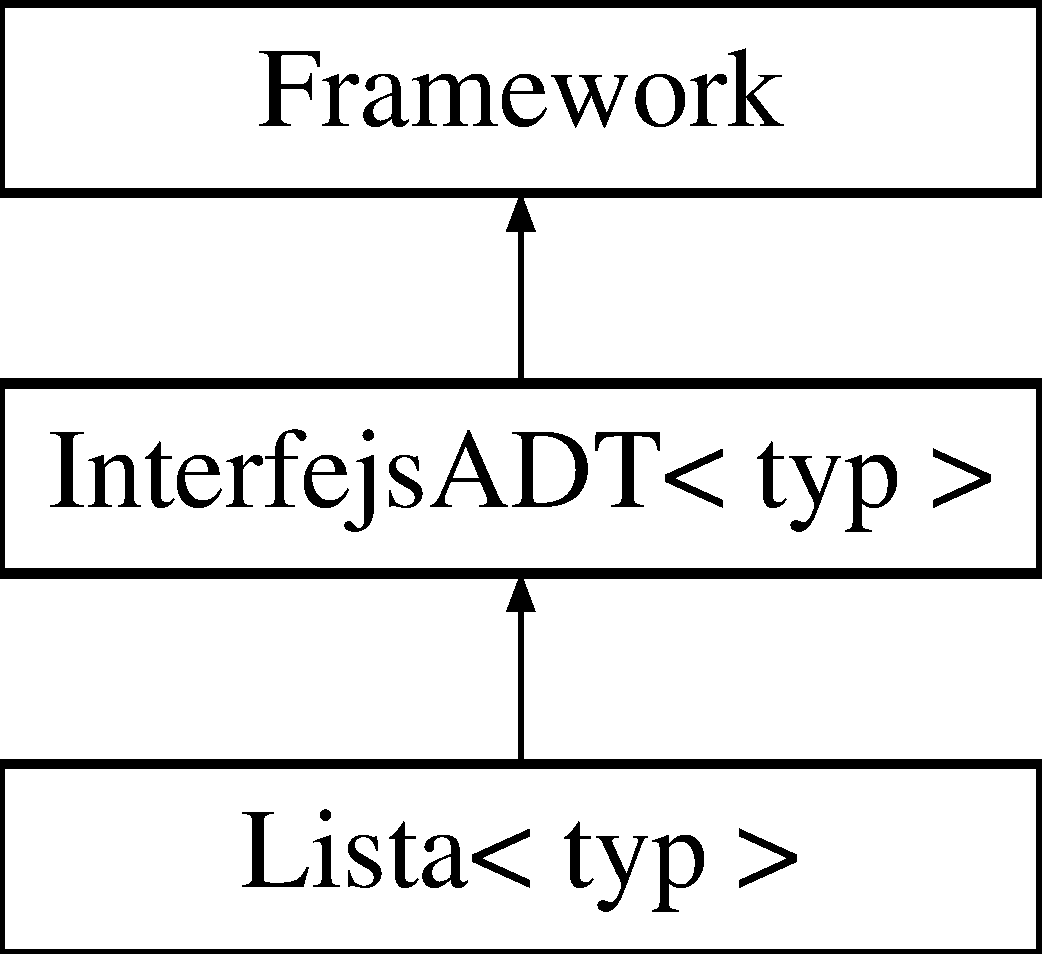
\includegraphics[height=2.564885cm]{class_framework}
\end{center}
\end{figure}
\subsubsection*{Public Member Functions}
\begin{DoxyCompactItemize}
\item 
virtual void \hyperlink{class_framework_a6ca4333f327109885071b5291486b492}{Wczytaj\-Dane} (const std\-::string nazwa\-Pliku, unsigned int n)=0
\begin{DoxyCompactList}\small\item\em Wczytanie danych z pliku. \end{DoxyCompactList}\item 
virtual void \hyperlink{class_framework_a883b9c2c7258021f9e8c55e02a9d8c60}{Start\-Msort} (unsigned int k)=0
\begin{DoxyCompactList}\small\item\em Wykonanie części obliczeniowej programu. \end{DoxyCompactList}\item 
virtual void \hyperlink{class_framework_a4d29e27b546088b26c1645a53adff349}{Start} ()=0
\item 
virtual void \hyperlink{class_framework_a6ae437019d35e0524adbeecc484f327a}{Zwolnij} ()=0
\begin{DoxyCompactList}\small\item\em Zwalnia pamięć po teście. \end{DoxyCompactList}\item 
virtual void \hyperlink{class_framework_ac1aff3a993eda9a110495d4a9d636900}{Pokaz} ()=0
\end{DoxyCompactItemize}


\subsubsection{Detailed Description}
Modeluje interfejs programu. 

Modeluje interfejs do programów wykonywanch w ramach kursu. 

Definition at line 24 of file Framework.\-hh.



\subsubsection{Member Function Documentation}
\hypertarget{class_framework_ac1aff3a993eda9a110495d4a9d636900}{\index{Framework@{Framework}!Pokaz@{Pokaz}}
\index{Pokaz@{Pokaz}!Framework@{Framework}}
\paragraph[{Pokaz}]{\setlength{\rightskip}{0pt plus 5cm}virtual void Framework\-::\-Pokaz (
\begin{DoxyParamCaption}
{}
\end{DoxyParamCaption}
)\hspace{0.3cm}{\ttfamily [pure virtual]}}}\label{class_framework_ac1aff3a993eda9a110495d4a9d636900}


Implemented in \hyperlink{class_list_arr2x_a5f2644455c4c3a1ee9f1752a74857241}{List\-Arr2x$<$ typ $>$}, and \hyperlink{class_interfejs_a_d_t_a22e091ad4cdcade33f9fa579a90ebf79}{Interfejs\-A\-D\-T$<$ typ $>$}.

\hypertarget{class_framework_a4d29e27b546088b26c1645a53adff349}{\index{Framework@{Framework}!Start@{Start}}
\index{Start@{Start}!Framework@{Framework}}
\paragraph[{Start}]{\setlength{\rightskip}{0pt plus 5cm}virtual void Framework\-::\-Start (
\begin{DoxyParamCaption}
{}
\end{DoxyParamCaption}
)\hspace{0.3cm}{\ttfamily [pure virtual]}}}\label{class_framework_a4d29e27b546088b26c1645a53adff349}


Implemented in \hyperlink{class_list_arr2x_ad73276a597d78b636119378ee408129d}{List\-Arr2x$<$ typ $>$}, and \hyperlink{class_interfejs_a_d_t_ae4f4f725bf09c5b258bc0d12e0f589d8}{Interfejs\-A\-D\-T$<$ typ $>$}.

\hypertarget{class_framework_a883b9c2c7258021f9e8c55e02a9d8c60}{\index{Framework@{Framework}!Start\-Msort@{Start\-Msort}}
\index{Start\-Msort@{Start\-Msort}!Framework@{Framework}}
\paragraph[{Start\-Msort}]{\setlength{\rightskip}{0pt plus 5cm}virtual void Framework\-::\-Start\-Msort (
\begin{DoxyParamCaption}
\item[{unsigned int}]{k}
\end{DoxyParamCaption}
)\hspace{0.3cm}{\ttfamily [pure virtual]}}}\label{class_framework_a883b9c2c7258021f9e8c55e02a9d8c60}


Wykonanie części obliczeniowej programu. 

Metoda w której implementowana jest część obliczeniowa programu, której czas wykonania zostanie zmierzony.


\begin{DoxyParams}[1]{Parameters}
\mbox{\tt in}  & {\em k} & -\/ ilość elementów dla których mają zostać wykonane obliczenia. \\
\hline
\end{DoxyParams}


Implemented in \hyperlink{class_list_arr2x_adfd1dd69dadd19ac04ede03dba454fb5}{List\-Arr2x$<$ typ $>$}, and \hyperlink{class_interfejs_a_d_t_a7fc6b6c9b0606a24846b7e744ee8a823}{Interfejs\-A\-D\-T$<$ typ $>$}.

\hypertarget{class_framework_a6ca4333f327109885071b5291486b492}{\index{Framework@{Framework}!Wczytaj\-Dane@{Wczytaj\-Dane}}
\index{Wczytaj\-Dane@{Wczytaj\-Dane}!Framework@{Framework}}
\paragraph[{Wczytaj\-Dane}]{\setlength{\rightskip}{0pt plus 5cm}virtual void Framework\-::\-Wczytaj\-Dane (
\begin{DoxyParamCaption}
\item[{const std\-::string}]{nazwa\-Pliku, }
\item[{unsigned int}]{n}
\end{DoxyParamCaption}
)\hspace{0.3cm}{\ttfamily [pure virtual]}}}\label{class_framework_a6ca4333f327109885071b5291486b492}


Wczytanie danych z pliku. 

Wczytuje zadaną ilość danych do przetworzenia z pliku o zadanej nazwie.


\begin{DoxyParams}[1]{Parameters}
\mbox{\tt in}  & {\em nazwa\-Pliku} & -\/ nazwa pliku z danymi \\
\hline
\mbox{\tt in}  & {\em n} & -\/ ilość danych do wczytania \\
\hline
\end{DoxyParams}


Implemented in \hyperlink{class_list_arr2x_afd6469fa733da21b70981fa4dfae9c12}{List\-Arr2x$<$ typ $>$}, and \hyperlink{class_interfejs_a_d_t_ae37b5d3abf3a7a85adf02e42e09df875}{Interfejs\-A\-D\-T$<$ typ $>$}.

\hypertarget{class_framework_a6ae437019d35e0524adbeecc484f327a}{\index{Framework@{Framework}!Zwolnij@{Zwolnij}}
\index{Zwolnij@{Zwolnij}!Framework@{Framework}}
\paragraph[{Zwolnij}]{\setlength{\rightskip}{0pt plus 5cm}virtual void Framework\-::\-Zwolnij (
\begin{DoxyParamCaption}
{}
\end{DoxyParamCaption}
)\hspace{0.3cm}{\ttfamily [pure virtual]}}}\label{class_framework_a6ae437019d35e0524adbeecc484f327a}


Zwalnia pamięć po teście. 

Zwalnia pamięć zajmowaną przez objekty wykorzytsane do testów 

Implemented in \hyperlink{class_list_arr2x_a4e922603e7ed26334ee19cbca3c5056d}{List\-Arr2x$<$ typ $>$}, \hyperlink{class_list_arr1_a613d2338847bd5d3b1383892d74280e7}{List\-Arr1$<$ typ $>$}, \hyperlink{class_kolejka_a87be5cc66cf0f4c813b489c0a11c4b35}{Kolejka$<$ typ $>$}, \hyperlink{class_lista_afcc18699707e00f35d73fa53eaa9f1da}{Lista$<$ typ $>$}, \hyperlink{class_stos_a1cfa859cdeddb64a9b49ec7526c5ac5a}{Stos$<$ typ $>$}, and \hyperlink{class_interfejs_a_d_t_a75427479b00e3d4a0c5f9615216262ea}{Interfejs\-A\-D\-T$<$ typ $>$}.



The documentation for this class was generated from the following file\-:\begin{DoxyCompactItemize}
\item 
/home/bartolomeo/209296/prj/inc/\hyperlink{_framework_8hh}{Framework.\-hh}\end{DoxyCompactItemize}

\hypertarget{class_interfejs_a_d_t}{\subsection{Interfejs\-A\-D\-T$<$ typ $>$ Class Template Reference}
\label{class_interfejs_a_d_t}\index{Interfejs\-A\-D\-T$<$ typ $>$@{Interfejs\-A\-D\-T$<$ typ $>$}}
}


{\ttfamily \#include $<$Interfejs\-A\-D\-T.\-hh$>$}

Inheritance diagram for Interfejs\-A\-D\-T$<$ typ $>$\-:\begin{figure}[H]
\begin{center}
\leavevmode
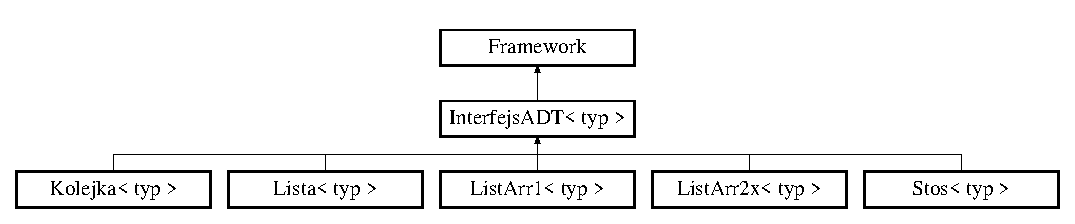
\includegraphics[height=2.564885cm]{class_interfejs_a_d_t}
\end{center}
\end{figure}
\subsubsection*{Public Member Functions}
\begin{DoxyCompactItemize}
\item 
virtual void \hyperlink{class_interfejs_a_d_t_abae6ef55c501edc4ca4e0faf4436b0df}{push} (typ dana, unsigned int pole)=0
\begin{DoxyCompactList}\small\item\em Dodaje kolejny element. \end{DoxyCompactList}\item 
virtual typ \hyperlink{class_interfejs_a_d_t_aa5a81a01c32577d986320524bcd091f0}{pop} (unsigned int pole)=0
\begin{DoxyCompactList}\small\item\em Pobiera element. \end{DoxyCompactList}\item 
virtual unsigned int \hyperlink{class_interfejs_a_d_t_a871cc26c895ce229ad04f7897fe4ba48}{size} ()=0
\begin{DoxyCompactList}\small\item\em Liczność elemetów. \end{DoxyCompactList}\item 
void \hyperlink{class_interfejs_a_d_t_ae37b5d3abf3a7a85adf02e42e09df875}{Wczytaj\-Dane} (const std\-::string nazwa\-Pliku, unsigned int n)=0
\begin{DoxyCompactList}\small\item\em Wczytanie danych z pliku. \end{DoxyCompactList}\item 
void \hyperlink{class_interfejs_a_d_t_a7fc6b6c9b0606a24846b7e744ee8a823}{Start\-Msort} (const unsigned int k)=0
\begin{DoxyCompactList}\small\item\em Wykonanie części obliczeniowej programu. \end{DoxyCompactList}\item 
void \hyperlink{class_interfejs_a_d_t_ae4f4f725bf09c5b258bc0d12e0f589d8}{Start} ()=0
\item 
virtual void \hyperlink{class_interfejs_a_d_t_a75427479b00e3d4a0c5f9615216262ea}{Zwolnij} ()=0
\begin{DoxyCompactList}\small\item\em Zwalnia pamięć \end{DoxyCompactList}\item 
virtual void \hyperlink{class_interfejs_a_d_t_a22e091ad4cdcade33f9fa579a90ebf79}{Pokaz} ()=0
\end{DoxyCompactItemize}


\subsubsection{Detailed Description}
\subsubsection*{template$<$class typ$>$class Interfejs\-A\-D\-T$<$ typ $>$}

\textbackslash{} brief Definiuje interfejs użytkownika

Definiuje interfejs użytkownika dla listy, stosu i kolejki. 

Definition at line 13 of file Interfejs\-A\-D\-T.\-hh.



\subsubsection{Member Function Documentation}
\hypertarget{class_interfejs_a_d_t_a22e091ad4cdcade33f9fa579a90ebf79}{\index{Interfejs\-A\-D\-T@{Interfejs\-A\-D\-T}!Pokaz@{Pokaz}}
\index{Pokaz@{Pokaz}!InterfejsADT@{Interfejs\-A\-D\-T}}
\paragraph[{Pokaz}]{\setlength{\rightskip}{0pt plus 5cm}template$<$class typ $>$ virtual void {\bf Interfejs\-A\-D\-T}$<$ typ $>$\-::Pokaz (
\begin{DoxyParamCaption}
{}
\end{DoxyParamCaption}
)\hspace{0.3cm}{\ttfamily [pure virtual]}}}\label{class_interfejs_a_d_t_a22e091ad4cdcade33f9fa579a90ebf79}


Implements \hyperlink{class_framework_ac1aff3a993eda9a110495d4a9d636900}{Framework}.



Implemented in \hyperlink{class_list_arr2x_a5f2644455c4c3a1ee9f1752a74857241}{List\-Arr2x$<$ typ $>$}.

\hypertarget{class_interfejs_a_d_t_aa5a81a01c32577d986320524bcd091f0}{\index{Interfejs\-A\-D\-T@{Interfejs\-A\-D\-T}!pop@{pop}}
\index{pop@{pop}!InterfejsADT@{Interfejs\-A\-D\-T}}
\paragraph[{pop}]{\setlength{\rightskip}{0pt plus 5cm}template$<$class typ $>$ virtual typ {\bf Interfejs\-A\-D\-T}$<$ typ $>$\-::pop (
\begin{DoxyParamCaption}
\item[{unsigned int}]{pole}
\end{DoxyParamCaption}
)\hspace{0.3cm}{\ttfamily [pure virtual]}}}\label{class_interfejs_a_d_t_aa5a81a01c32577d986320524bcd091f0}


Pobiera element. 

Pobiera element z typu danych


\begin{DoxyParams}[1]{Parameters}
\mbox{\tt in}  & {\em pole} & -\/ !!!\-D\-O\-S\-T\-E\-P\-N\-E T\-Y\-L\-K\-O D\-L\-A L\-I\-S\-T\-Y!!! nr pola z ktore pobiera element\\
\hline
\end{DoxyParams}

\begin{DoxyRetVals}{Return values}
{\em zwraca} & wartość danego elementu \\
\hline
\end{DoxyRetVals}


Implemented in \hyperlink{class_list_arr2x_a6462ac1f547b7a090e54629539ce2dda}{List\-Arr2x$<$ typ $>$}, \hyperlink{class_lista_aea1df940db61c9565cc6f95a6d3df202}{Lista$<$ typ $>$}, \hyperlink{class_kolejka_a9c41aaf09b6a9a336e33cb49486a2bf8}{Kolejka$<$ typ $>$}, \hyperlink{class_stos_ab18e88e29805390208e6587e7858ced1}{Stos$<$ typ $>$}, and \hyperlink{class_list_arr1_acbc2f02d8ee4389cfd202beeddfae82c}{List\-Arr1$<$ typ $>$}.

\hypertarget{class_interfejs_a_d_t_abae6ef55c501edc4ca4e0faf4436b0df}{\index{Interfejs\-A\-D\-T@{Interfejs\-A\-D\-T}!push@{push}}
\index{push@{push}!InterfejsADT@{Interfejs\-A\-D\-T}}
\paragraph[{push}]{\setlength{\rightskip}{0pt plus 5cm}template$<$class typ $>$ virtual void {\bf Interfejs\-A\-D\-T}$<$ typ $>$\-::push (
\begin{DoxyParamCaption}
\item[{typ}]{dana, }
\item[{unsigned int}]{pole}
\end{DoxyParamCaption}
)\hspace{0.3cm}{\ttfamily [pure virtual]}}}\label{class_interfejs_a_d_t_abae6ef55c501edc4ca4e0faf4436b0df}


Dodaje kolejny element. 

Dodaje kolejny element do typu danych


\begin{DoxyParams}[1]{Parameters}
\mbox{\tt in}  & {\em dana} & -\/ element który chcemy dorzucić do naszego typu \\
\hline
\mbox{\tt in}  & {\em pole} & -\/ !!!\-D\-O\-S\-T\-E\-P\-N\-E T\-Y\-L\-K\-O D\-L\-A L\-I\-S\-T\-Y!!! nr pola na które chcemy dodać element \\
\hline
\end{DoxyParams}


Implemented in \hyperlink{class_list_arr2x_a6aa004e56bdaf72de719d682b4069011}{List\-Arr2x$<$ typ $>$}, \hyperlink{class_kolejka_a9a58ac1ae2cd978f29cc31343e437343}{Kolejka$<$ typ $>$}, \hyperlink{class_lista_a4f6959cec316c8882a1dfc64d92480c1}{Lista$<$ typ $>$}, \hyperlink{class_stos_aa365a8b36117a4ebc99236de643a3354}{Stos$<$ typ $>$}, and \hyperlink{class_list_arr1_a9b8bfbeae4e0b93ab47398d0282447b5}{List\-Arr1$<$ typ $>$}.

\hypertarget{class_interfejs_a_d_t_a871cc26c895ce229ad04f7897fe4ba48}{\index{Interfejs\-A\-D\-T@{Interfejs\-A\-D\-T}!size@{size}}
\index{size@{size}!InterfejsADT@{Interfejs\-A\-D\-T}}
\paragraph[{size}]{\setlength{\rightskip}{0pt plus 5cm}template$<$class typ $>$ virtual unsigned int {\bf Interfejs\-A\-D\-T}$<$ typ $>$\-::size (
\begin{DoxyParamCaption}
{}
\end{DoxyParamCaption}
)\hspace{0.3cm}{\ttfamily [pure virtual]}}}\label{class_interfejs_a_d_t_a871cc26c895ce229ad04f7897fe4ba48}


Liczność elemetów. 

Informuje o licznośći elementów obecnie przechowywanych


\begin{DoxyRetVals}{Return values}
{\em zwraca} & ilość przechowywanych elementów \\
\hline
\end{DoxyRetVals}


Implemented in \hyperlink{class_list_arr2x_a6097d85211e74053506d4a5dce86f26c}{List\-Arr2x$<$ typ $>$}, \hyperlink{class_lista_a29244b4a79de727a53c23e84bca6d61e}{Lista$<$ typ $>$}, \hyperlink{class_kolejka_aed97a8e2e6d7092a36cdc55c89df64f2}{Kolejka$<$ typ $>$}, \hyperlink{class_stos_aea130eb6d93369ac9f8cc5936509a4c1}{Stos$<$ typ $>$}, and \hyperlink{class_list_arr1_a42b97b706c07e85f866bafd6ebc9b440}{List\-Arr1$<$ typ $>$}.

\hypertarget{class_interfejs_a_d_t_ae4f4f725bf09c5b258bc0d12e0f589d8}{\index{Interfejs\-A\-D\-T@{Interfejs\-A\-D\-T}!Start@{Start}}
\index{Start@{Start}!InterfejsADT@{Interfejs\-A\-D\-T}}
\paragraph[{Start}]{\setlength{\rightskip}{0pt plus 5cm}template$<$class typ $>$ void {\bf Interfejs\-A\-D\-T}$<$ typ $>$\-::Start (
\begin{DoxyParamCaption}
{}
\end{DoxyParamCaption}
)\hspace{0.3cm}{\ttfamily [pure virtual]}}}\label{class_interfejs_a_d_t_ae4f4f725bf09c5b258bc0d12e0f589d8}


Implements \hyperlink{class_framework_a4d29e27b546088b26c1645a53adff349}{Framework}.



Implemented in \hyperlink{class_list_arr2x_ad73276a597d78b636119378ee408129d}{List\-Arr2x$<$ typ $>$}.

\hypertarget{class_interfejs_a_d_t_a7fc6b6c9b0606a24846b7e744ee8a823}{\index{Interfejs\-A\-D\-T@{Interfejs\-A\-D\-T}!Start\-Msort@{Start\-Msort}}
\index{Start\-Msort@{Start\-Msort}!InterfejsADT@{Interfejs\-A\-D\-T}}
\paragraph[{Start\-Msort}]{\setlength{\rightskip}{0pt plus 5cm}template$<$class typ $>$ void {\bf Interfejs\-A\-D\-T}$<$ typ $>$\-::Start\-Msort (
\begin{DoxyParamCaption}
\item[{const unsigned int}]{k}
\end{DoxyParamCaption}
)\hspace{0.3cm}{\ttfamily [pure virtual]}}}\label{class_interfejs_a_d_t_a7fc6b6c9b0606a24846b7e744ee8a823}


Wykonanie części obliczeniowej programu. 

Metoda w której implementowana jest część obliczeniowa programu, której czas wykonania zostanie zmierzony.


\begin{DoxyParams}[1]{Parameters}
\mbox{\tt in}  & {\em k} & -\/ ilość elementów dla których mają zostać wykonane obliczenia. \\
\hline
\end{DoxyParams}


Implements \hyperlink{class_framework_a883b9c2c7258021f9e8c55e02a9d8c60}{Framework}.



Implemented in \hyperlink{class_list_arr2x_adfd1dd69dadd19ac04ede03dba454fb5}{List\-Arr2x$<$ typ $>$}.

\hypertarget{class_interfejs_a_d_t_ae37b5d3abf3a7a85adf02e42e09df875}{\index{Interfejs\-A\-D\-T@{Interfejs\-A\-D\-T}!Wczytaj\-Dane@{Wczytaj\-Dane}}
\index{Wczytaj\-Dane@{Wczytaj\-Dane}!InterfejsADT@{Interfejs\-A\-D\-T}}
\paragraph[{Wczytaj\-Dane}]{\setlength{\rightskip}{0pt plus 5cm}template$<$class typ $>$ void {\bf Interfejs\-A\-D\-T}$<$ typ $>$\-::Wczytaj\-Dane (
\begin{DoxyParamCaption}
\item[{const std\-::string}]{nazwa\-Pliku, }
\item[{unsigned int}]{n}
\end{DoxyParamCaption}
)\hspace{0.3cm}{\ttfamily [pure virtual]}}}\label{class_interfejs_a_d_t_ae37b5d3abf3a7a85adf02e42e09df875}


Wczytanie danych z pliku. 

Wczytuje zadaną ilość danych do przetworzenia z pliku o zadanej nazwie.


\begin{DoxyParams}[1]{Parameters}
\mbox{\tt in}  & {\em nazwa\-Pliku} & -\/ nazwa pliku z danymi \\
\hline
\mbox{\tt in}  & {\em n} & -\/ ilość danych do wczytania \\
\hline
\end{DoxyParams}


Implements \hyperlink{class_framework_a6ca4333f327109885071b5291486b492}{Framework}.



Implemented in \hyperlink{class_list_arr2x_afd6469fa733da21b70981fa4dfae9c12}{List\-Arr2x$<$ typ $>$}.

\hypertarget{class_interfejs_a_d_t_a75427479b00e3d4a0c5f9615216262ea}{\index{Interfejs\-A\-D\-T@{Interfejs\-A\-D\-T}!Zwolnij@{Zwolnij}}
\index{Zwolnij@{Zwolnij}!InterfejsADT@{Interfejs\-A\-D\-T}}
\paragraph[{Zwolnij}]{\setlength{\rightskip}{0pt plus 5cm}template$<$class typ $>$ virtual void {\bf Interfejs\-A\-D\-T}$<$ typ $>$\-::Zwolnij (
\begin{DoxyParamCaption}
{}
\end{DoxyParamCaption}
)\hspace{0.3cm}{\ttfamily [pure virtual]}}}\label{class_interfejs_a_d_t_a75427479b00e3d4a0c5f9615216262ea}


Zwalnia pamięć 

Zwalnia pamięć zajmowaną przez daną strukturę 

Implements \hyperlink{class_framework_a6ae437019d35e0524adbeecc484f327a}{Framework}.



Implemented in \hyperlink{class_list_arr2x_a4e922603e7ed26334ee19cbca3c5056d}{List\-Arr2x$<$ typ $>$}, \hyperlink{class_list_arr1_a613d2338847bd5d3b1383892d74280e7}{List\-Arr1$<$ typ $>$}, \hyperlink{class_kolejka_a87be5cc66cf0f4c813b489c0a11c4b35}{Kolejka$<$ typ $>$}, \hyperlink{class_lista_afcc18699707e00f35d73fa53eaa9f1da}{Lista$<$ typ $>$}, and \hyperlink{class_stos_a1cfa859cdeddb64a9b49ec7526c5ac5a}{Stos$<$ typ $>$}.



The documentation for this class was generated from the following file\-:\begin{DoxyCompactItemize}
\item 
/home/bartolomeo/209296/prj/inc/\hyperlink{_interfejs_a_d_t_8hh}{Interfejs\-A\-D\-T.\-hh}\end{DoxyCompactItemize}

\hypertarget{class_kolejka}{\subsection{Kolejka$<$ typ $>$ Class Template Reference}
\label{class_kolejka}\index{Kolejka$<$ typ $>$@{Kolejka$<$ typ $>$}}
}


Modeluje pojęcie Kolejki.  




{\ttfamily \#include $<$Kolejka.\-hh$>$}

Inheritance diagram for Kolejka$<$ typ $>$\-:\begin{figure}[H]
\begin{center}
\leavevmode
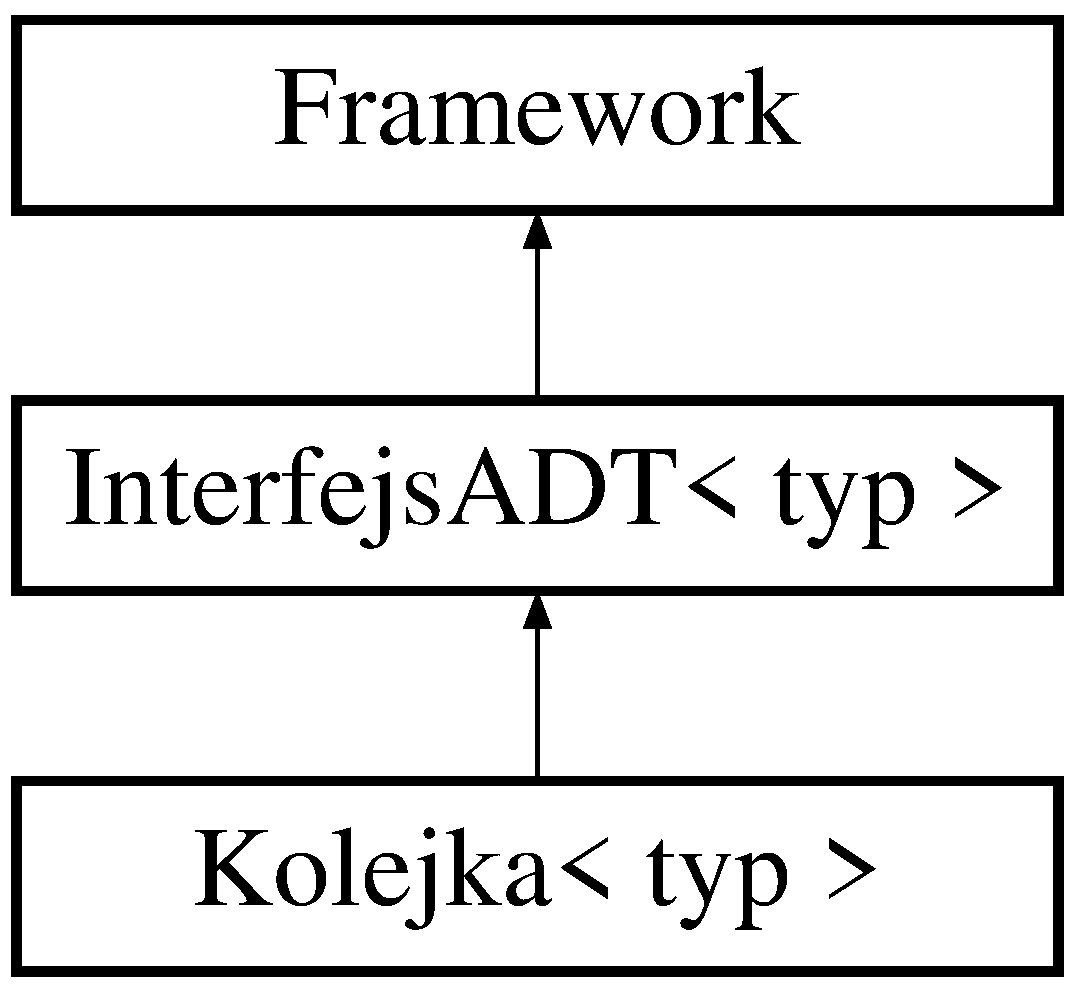
\includegraphics[height=3.000000cm]{class_kolejka}
\end{center}
\end{figure}
\subsubsection*{Classes}
\begin{DoxyCompactItemize}
\item 
struct \hyperlink{struct_kolejka_1_1_element}{Element}
\begin{DoxyCompactList}\small\item\em Modeluje jeden element Kolejki. \end{DoxyCompactList}\end{DoxyCompactItemize}
\subsubsection*{Public Member Functions}
\begin{DoxyCompactItemize}
\item 
\hyperlink{class_kolejka_ae64d506b36a27fdf2c66e53aaa7ae79d}{Kolejka} ()
\begin{DoxyCompactList}\small\item\em Konstruktor pustej Kolejki. \end{DoxyCompactList}\item 
void \hyperlink{class_kolejka_a87be5cc66cf0f4c813b489c0a11c4b35}{Zwolnij} ()
\begin{DoxyCompactList}\small\item\em Destruktor Kolejki. \end{DoxyCompactList}\item 
void \hyperlink{class_kolejka_a9a58ac1ae2cd978f29cc31343e437343}{push} (typ dana, unsigned int pole=0)
\begin{DoxyCompactList}\small\item\em Dodaje daną do Kolejki. \end{DoxyCompactList}\item 
void \hyperlink{class_kolejka_a9c41aaf09b6a9a336e33cb49486a2bf8}{pop} (unsigned int pole=0)
\begin{DoxyCompactList}\small\item\em Usuwa element z Kolejki. \end{DoxyCompactList}\item 
unsigned int \hyperlink{class_kolejka_aed97a8e2e6d7092a36cdc55c89df64f2}{size} ()
\begin{DoxyCompactList}\small\item\em Sprawdza rozmiar Kolejki. \end{DoxyCompactList}\item 
void \hyperlink{class_kolejka_aed2f002e78d62b2680023114c4cef18f}{Wczytaj\-Dane} (const char $\ast$nazwa\-Pliku, unsigned int n)
\begin{DoxyCompactList}\small\item\em Wczytuje dane z pliku. \end{DoxyCompactList}\item 
void \hyperlink{class_kolejka_a5a8c5757bdb72a76b004891d393adc94}{Start} (const unsigned int k)
\begin{DoxyCompactList}\small\item\em Proces obliczeniowy. \end{DoxyCompactList}\end{DoxyCompactItemize}
\subsubsection*{Private Attributes}
\begin{DoxyCompactItemize}
\item 
\hyperlink{struct_kolejka_1_1_element}{Element} $\ast$ \hyperlink{class_kolejka_aa061333b7e9f42c5782761cb15ef6ea3}{Poczatek}
\begin{DoxyCompactList}\small\item\em Wskaźnik na pierwszy element Kolejki. \end{DoxyCompactList}\item 
\hyperlink{struct_kolejka_1_1_element}{Element} $\ast$ \hyperlink{class_kolejka_abc6056d0a1f4d021efd89c0152cbc594}{Koniec}
\begin{DoxyCompactList}\small\item\em Wskaźnik na ostatni element Kolejki. \end{DoxyCompactList}\item 
unsigned int \hyperlink{class_kolejka_ad5de4ece31be7fed6ad5fd0bbe9c3765}{Rozmiar}
\begin{DoxyCompactList}\small\item\em Aktualny rozmiar Kolejki. \end{DoxyCompactList}\end{DoxyCompactItemize}


\subsubsection{Detailed Description}
\subsubsection*{template$<$class typ$>$class Kolejka$<$ typ $>$}

Modeluje pojęcie Kolejki. 

Modeluje pojęcie Kolejki zadeklarowanego w szablonie typu Uwaga! Kolejkę indeksujemy od 0. 

Definition at line 25 of file Kolejka.\-hh.



\subsubsection{Constructor \& Destructor Documentation}
\hypertarget{class_kolejka_ae64d506b36a27fdf2c66e53aaa7ae79d}{\index{Kolejka@{Kolejka}!Kolejka@{Kolejka}}
\index{Kolejka@{Kolejka}!Kolejka@{Kolejka}}
\paragraph[{Kolejka}]{\setlength{\rightskip}{0pt plus 5cm}template$<$class typ $>$ {\bf Kolejka}$<$ typ $>$\-::{\bf Kolejka} (
\begin{DoxyParamCaption}
{}
\end{DoxyParamCaption}
)\hspace{0.3cm}{\ttfamily [inline]}}}\label{class_kolejka_ae64d506b36a27fdf2c66e53aaa7ae79d}


Konstruktor pustej Kolejki. 

Konstruktor bezargumentowy pustej Kolejki tworzy objekt z wskaźnikiem początek pokazującym na N\-U\-L\-L. 

Definition at line 100 of file Kolejka.\-hh.



\subsubsection{Member Function Documentation}
\hypertarget{class_kolejka_a9c41aaf09b6a9a336e33cb49486a2bf8}{\index{Kolejka@{Kolejka}!pop@{pop}}
\index{pop@{pop}!Kolejka@{Kolejka}}
\paragraph[{pop}]{\setlength{\rightskip}{0pt plus 5cm}template$<$class typ $>$ void {\bf Kolejka}$<$ typ $>$\-::pop (
\begin{DoxyParamCaption}
\item[{unsigned int}]{pole = {\ttfamily 0}}
\end{DoxyParamCaption}
)\hspace{0.3cm}{\ttfamily [inline]}, {\ttfamily [virtual]}}}\label{class_kolejka_a9c41aaf09b6a9a336e33cb49486a2bf8}


Usuwa element z Kolejki. 

Usuwa pierwszy element z Kolejki U\-W\-A\-G\-A! Nie zmieniać drugiego argumentu wywołania, bądź ustawoć 0!


\begin{DoxyParams}[1]{Parameters}
\mbox{\tt in}  & {\em pole} & -\/ numer elementu w Kolejce którzy wyrzucimy, domyślnie 0, zmiana podczas wywołania nie ma wpływu na działanie metody; \\
\hline
\end{DoxyParams}


Implements \hyperlink{class_interfejs_a_d_t_aa5a81a01c32577d986320524bcd091f0}{Interfejs\-A\-D\-T$<$ typ $>$}.



Definition at line 173 of file Kolejka.\-hh.

\hypertarget{class_kolejka_a9a58ac1ae2cd978f29cc31343e437343}{\index{Kolejka@{Kolejka}!push@{push}}
\index{push@{push}!Kolejka@{Kolejka}}
\paragraph[{push}]{\setlength{\rightskip}{0pt plus 5cm}template$<$class typ $>$ void {\bf Kolejka}$<$ typ $>$\-::push (
\begin{DoxyParamCaption}
\item[{typ}]{dana, }
\item[{unsigned int}]{pole = {\ttfamily 0}}
\end{DoxyParamCaption}
)\hspace{0.3cm}{\ttfamily [inline]}, {\ttfamily [virtual]}}}\label{class_kolejka_a9a58ac1ae2cd978f29cc31343e437343}


Dodaje daną do Kolejki. 

Dodaje daną podaną jako pierwszy argument wywołania na koniec Kolejki Uwaga! nie zmieniać drugiego argumentu wywołania!


\begin{DoxyParams}[1]{Parameters}
\mbox{\tt in}  & {\em dana} & -\/ dana którą chcemy dodać do Kolejki \\
\hline
\mbox{\tt in}  & {\em pole} & -\/ numer miejsca gdzie zostanie dodany element -\/ domyślnie koniec koelejki, zmiana arumentu podczas wywowłania nie wpływa na działanie metody. \\
\hline
\end{DoxyParams}


Implements \hyperlink{class_interfejs_a_d_t_abae6ef55c501edc4ca4e0faf4436b0df}{Interfejs\-A\-D\-T$<$ typ $>$}.



Definition at line 146 of file Kolejka.\-hh.

\hypertarget{class_kolejka_aed97a8e2e6d7092a36cdc55c89df64f2}{\index{Kolejka@{Kolejka}!size@{size}}
\index{size@{size}!Kolejka@{Kolejka}}
\paragraph[{size}]{\setlength{\rightskip}{0pt plus 5cm}template$<$class typ $>$ unsigned int {\bf Kolejka}$<$ typ $>$\-::size (
\begin{DoxyParamCaption}
{}
\end{DoxyParamCaption}
)\hspace{0.3cm}{\ttfamily [inline]}, {\ttfamily [virtual]}}}\label{class_kolejka_aed97a8e2e6d7092a36cdc55c89df64f2}


Sprawdza rozmiar Kolejki. 

Sprawdza ile aktualnie elementów znajduję się w Kolejce


\begin{DoxyRetVals}{Return values}
{\em zwraca} & ilosć elementów znadjuących się aktualnie w Kolejce \\
\hline
\end{DoxyRetVals}


Implements \hyperlink{class_interfejs_a_d_t_a871cc26c895ce229ad04f7897fe4ba48}{Interfejs\-A\-D\-T$<$ typ $>$}.



Definition at line 194 of file Kolejka.\-hh.

\hypertarget{class_kolejka_a5a8c5757bdb72a76b004891d393adc94}{\index{Kolejka@{Kolejka}!Start@{Start}}
\index{Start@{Start}!Kolejka@{Kolejka}}
\paragraph[{Start}]{\setlength{\rightskip}{0pt plus 5cm}template$<$class typ $>$ void {\bf Kolejka}$<$ typ $>$\-::Start (
\begin{DoxyParamCaption}
\item[{const unsigned int}]{k}
\end{DoxyParamCaption}
)\hspace{0.3cm}{\ttfamily [inline]}}}\label{class_kolejka_a5a8c5757bdb72a76b004891d393adc94}


Proces obliczeniowy. 

Wykonuje proces oblcizeniowy, którego czas wykonania jest mierzony na potrzeby laboratoriów P\-A\-M\-S\-I W tym wypakdu tworzy Kolejkę k elementową wypełnioną stałą liczbą '3'.


\begin{DoxyParams}[1]{Parameters}
\mbox{\tt in}  & {\em k} & -\/ ilość danych dla których ma zostać przeprowadzona precedura obnliczeniowa \\
\hline
\end{DoxyParams}


Definition at line 220 of file Kolejka.\-hh.

\hypertarget{class_kolejka_aed2f002e78d62b2680023114c4cef18f}{\index{Kolejka@{Kolejka}!Wczytaj\-Dane@{Wczytaj\-Dane}}
\index{Wczytaj\-Dane@{Wczytaj\-Dane}!Kolejka@{Kolejka}}
\paragraph[{Wczytaj\-Dane}]{\setlength{\rightskip}{0pt plus 5cm}template$<$class typ $>$ void {\bf Kolejka}$<$ typ $>$\-::Wczytaj\-Dane (
\begin{DoxyParamCaption}
\item[{const char $\ast$}]{nazwa\-Pliku, }
\item[{unsigned int}]{n}
\end{DoxyParamCaption}
)\hspace{0.3cm}{\ttfamily [inline]}}}\label{class_kolejka_aed2f002e78d62b2680023114c4cef18f}


Wczytuje dane z pliku. 

Wczytuje dane zamieszczone w pliku do Kolejki. Każdą nową daną umieszcza na końcu Kolejki.


\begin{DoxyParams}[1]{Parameters}
\mbox{\tt in}  & {\em nazwa\-Pliku} & -\/ nazwa pliku z danymi \\
\hline
\mbox{\tt in}  & {\em n} & -\/ ilość danych do wczytania \\
\hline
\end{DoxyParams}


Definition at line 206 of file Kolejka.\-hh.

\hypertarget{class_kolejka_a87be5cc66cf0f4c813b489c0a11c4b35}{\index{Kolejka@{Kolejka}!Zwolnij@{Zwolnij}}
\index{Zwolnij@{Zwolnij}!Kolejka@{Kolejka}}
\paragraph[{Zwolnij}]{\setlength{\rightskip}{0pt plus 5cm}template$<$class typ $>$ void {\bf Kolejka}$<$ typ $>$\-::Zwolnij (
\begin{DoxyParamCaption}
{}
\end{DoxyParamCaption}
)\hspace{0.3cm}{\ttfamily [inline]}, {\ttfamily [virtual]}}}\label{class_kolejka_a87be5cc66cf0f4c813b489c0a11c4b35}


Destruktor Kolejki. 

Zwalnia zaalokowana przez Kolejke pamiec

Zwalnia pamięć

Zwalnia pamięć zajmowaną przez Kolejkę 

Implements \hyperlink{class_interfejs_a_d_t_a75427479b00e3d4a0c5f9615216262ea}{Interfejs\-A\-D\-T$<$ typ $>$}.



Definition at line 124 of file Kolejka.\-hh.



\subsubsection{Member Data Documentation}
\hypertarget{class_kolejka_abc6056d0a1f4d021efd89c0152cbc594}{\index{Kolejka@{Kolejka}!Koniec@{Koniec}}
\index{Koniec@{Koniec}!Kolejka@{Kolejka}}
\paragraph[{Koniec}]{\setlength{\rightskip}{0pt plus 5cm}template$<$class typ $>$ {\bf Element}$\ast$ {\bf Kolejka}$<$ typ $>$\-::Koniec\hspace{0.3cm}{\ttfamily [private]}}}\label{class_kolejka_abc6056d0a1f4d021efd89c0152cbc594}


Wskaźnik na ostatni element Kolejki. 

Wskaźnik na ostatni element kolejki zwiększający szybkowść dodawania danych na końcu 

Definition at line 81 of file Kolejka.\-hh.

\hypertarget{class_kolejka_aa061333b7e9f42c5782761cb15ef6ea3}{\index{Kolejka@{Kolejka}!Poczatek@{Poczatek}}
\index{Poczatek@{Poczatek}!Kolejka@{Kolejka}}
\paragraph[{Poczatek}]{\setlength{\rightskip}{0pt plus 5cm}template$<$class typ $>$ {\bf Element}$\ast$ {\bf Kolejka}$<$ typ $>$\-::Poczatek\hspace{0.3cm}{\ttfamily [private]}}}\label{class_kolejka_aa061333b7e9f42c5782761cb15ef6ea3}


Wskaźnik na pierwszy element Kolejki. 

Wskaźnik na pierwszy element Kolejki 

Definition at line 72 of file Kolejka.\-hh.

\hypertarget{class_kolejka_ad5de4ece31be7fed6ad5fd0bbe9c3765}{\index{Kolejka@{Kolejka}!Rozmiar@{Rozmiar}}
\index{Rozmiar@{Rozmiar}!Kolejka@{Kolejka}}
\paragraph[{Rozmiar}]{\setlength{\rightskip}{0pt plus 5cm}template$<$class typ $>$ unsigned int {\bf Kolejka}$<$ typ $>$\-::Rozmiar\hspace{0.3cm}{\ttfamily [private]}}}\label{class_kolejka_ad5de4ece31be7fed6ad5fd0bbe9c3765}


Aktualny rozmiar Kolejki. 

Przechowuje aktualną ilość Elemenetów znajujących się w Kolejce 

Definition at line 88 of file Kolejka.\-hh.



The documentation for this class was generated from the following file\-:\begin{DoxyCompactItemize}
\item 
/home/bartolomeo/209296/prj/inc/\hyperlink{_kolejka_8hh}{Kolejka.\-hh}\end{DoxyCompactItemize}

\hypertarget{class_lista}{\subsection{Lista$<$ typ $>$ Class Template Reference}
\label{class_lista}\index{Lista$<$ typ $>$@{Lista$<$ typ $>$}}
}


Modeluje pojęcie listy.  




{\ttfamily \#include $<$Lista.\-hh$>$}

Inheritance diagram for Lista$<$ typ $>$\-:\begin{figure}[H]
\begin{center}
\leavevmode
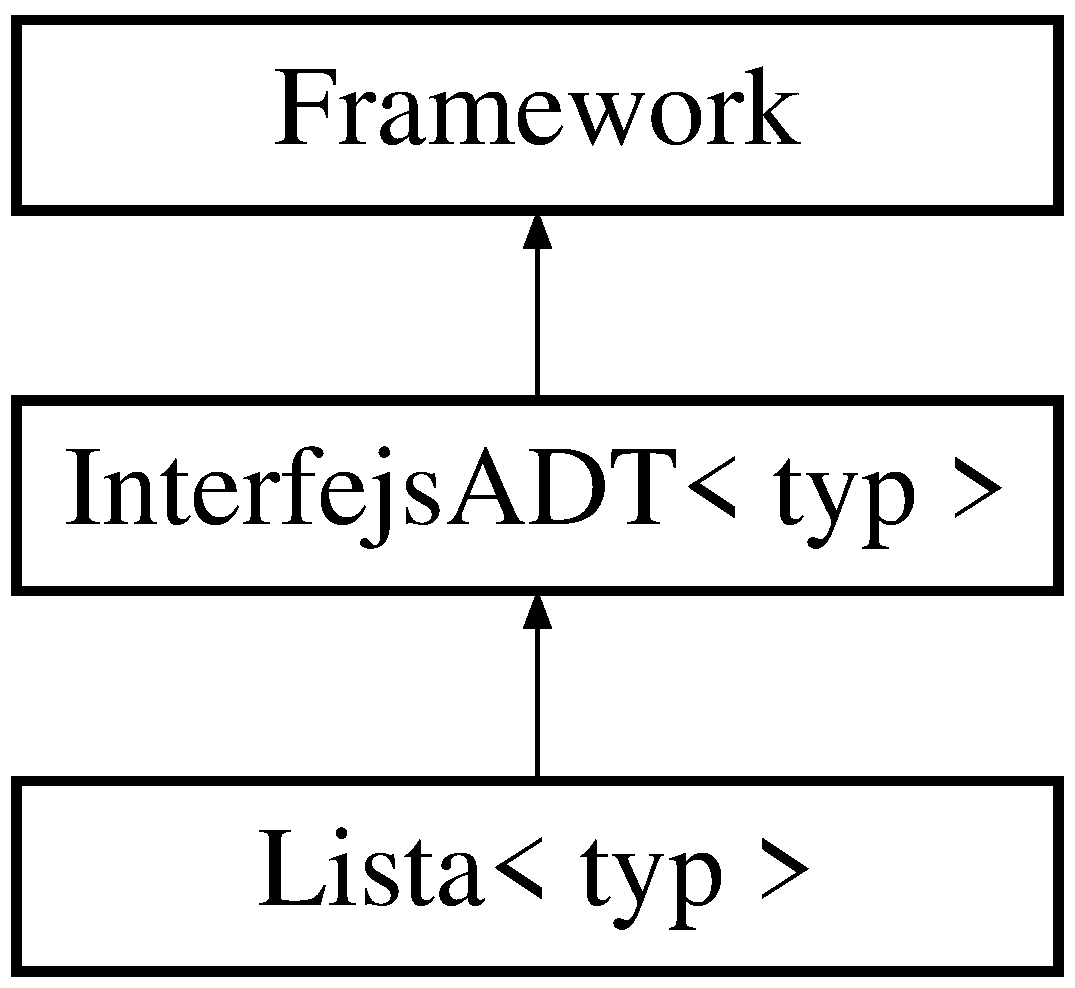
\includegraphics[height=3.000000cm]{class_lista}
\end{center}
\end{figure}
\subsubsection*{Classes}
\begin{DoxyCompactItemize}
\item 
struct \hyperlink{struct_lista_1_1_element}{Element}
\begin{DoxyCompactList}\small\item\em Modeluje jeden element Listy. \end{DoxyCompactList}\end{DoxyCompactItemize}
\subsubsection*{Public Member Functions}
\begin{DoxyCompactItemize}
\item 
\hyperlink{class_lista_a23a5b3313a893057276942e74f330b89}{Lista} ()
\begin{DoxyCompactList}\small\item\em Konstruktor puste listy. \end{DoxyCompactList}\item 
void \hyperlink{class_lista_afcc18699707e00f35d73fa53eaa9f1da}{Zwolnij} ()
\begin{DoxyCompactList}\small\item\em Destruktor listy. \end{DoxyCompactList}\item 
void \hyperlink{class_lista_a4f6959cec316c8882a1dfc64d92480c1}{push} (typ dana, unsigned int pole)
\begin{DoxyCompactList}\small\item\em Dodaje daną do Listy. \end{DoxyCompactList}\item 
typ \hyperlink{class_lista_aea1df940db61c9565cc6f95a6d3df202}{pop} (unsigned int pole)
\begin{DoxyCompactList}\small\item\em Usuwa element z Listy. \end{DoxyCompactList}\item 
unsigned int \hyperlink{class_lista_a29244b4a79de727a53c23e84bca6d61e}{size} ()
\begin{DoxyCompactList}\small\item\em Sprawdza rozmiar Listy. \end{DoxyCompactList}\item 
void \hyperlink{class_lista_a8dd8489d2db5ce989ffd71268a11e18c}{Wczytaj\-Dane} (const char $\ast$nazwa\-Pliku, unsigned int n=0)
\begin{DoxyCompactList}\small\item\em Wczytuje dane z pliku. \end{DoxyCompactList}\item 
typ \hyperlink{class_lista_a3ffb056a10d97afbe52bb8a3ba6fbb6a}{operator\mbox{[}$\,$\mbox{]}} (size\-\_\-t pole) const 
\begin{DoxyCompactList}\small\item\em Wyciąga wartość elementu Listy. \end{DoxyCompactList}\item 
void \hyperlink{class_lista_aa5f8153e21cbd4569f4e16a3c466e947}{Start} (const unsigned int k)
\begin{DoxyCompactList}\small\item\em Proces obliczeniowy. \end{DoxyCompactList}\end{DoxyCompactItemize}
\subsubsection*{Private Attributes}
\begin{DoxyCompactItemize}
\item 
\hyperlink{struct_lista_1_1_element}{Element} $\ast$ \hyperlink{class_lista_af0b9911cad81701e55a4290a3941fa29}{Poczatek}
\begin{DoxyCompactList}\small\item\em Wskaźnik na pierwszy element Listy. \end{DoxyCompactList}\item 
\hyperlink{struct_lista_1_1_element}{Element} $\ast$ \hyperlink{class_lista_a5c0ab4649945504ec400bb028f95ae1a}{Koniec}
\begin{DoxyCompactList}\small\item\em Wzkaźnik na ostatni element listy. \end{DoxyCompactList}\item 
unsigned int \hyperlink{class_lista_a3bc5134ce062dfd20cc7747d34f3ff16}{Rozmiar}
\begin{DoxyCompactList}\small\item\em Aktualny rozmiar Listy. \end{DoxyCompactList}\end{DoxyCompactItemize}


\subsubsection{Detailed Description}
\subsubsection*{template$<$class typ$>$class Lista$<$ typ $>$}

Modeluje pojęcie listy. 

Modeluje pojęcie listy zadeklarowanego w szablonie typu Uwaga! Listę indeksujemy od 0. 

Definition at line 24 of file Lista.\-hh.



\subsubsection{Constructor \& Destructor Documentation}
\hypertarget{class_lista_a23a5b3313a893057276942e74f330b89}{\index{Lista@{Lista}!Lista@{Lista}}
\index{Lista@{Lista}!Lista@{Lista}}
\paragraph[{Lista}]{\setlength{\rightskip}{0pt plus 5cm}template$<$class typ $>$ {\bf Lista}$<$ typ $>$\-::{\bf Lista} (
\begin{DoxyParamCaption}
{}
\end{DoxyParamCaption}
)\hspace{0.3cm}{\ttfamily [inline]}}}\label{class_lista_a23a5b3313a893057276942e74f330b89}


Konstruktor puste listy. 

Konstruktor bezargumentowy pustej listy tworzy objekt z wskaźnikiem początek pokazującym na N\-U\-L\-L. 

Definition at line 98 of file Lista.\-hh.



\subsubsection{Member Function Documentation}
\hypertarget{class_lista_a3ffb056a10d97afbe52bb8a3ba6fbb6a}{\index{Lista@{Lista}!operator\mbox{[}$\,$\mbox{]}@{operator[]}}
\index{operator\mbox{[}$\,$\mbox{]}@{operator[]}!Lista@{Lista}}
\paragraph[{operator[]}]{\setlength{\rightskip}{0pt plus 5cm}template$<$class typ $>$ typ {\bf Lista}$<$ typ $>$\-::operator\mbox{[}$\,$\mbox{]} (
\begin{DoxyParamCaption}
\item[{size\-\_\-t}]{pole}
\end{DoxyParamCaption}
) const\hspace{0.3cm}{\ttfamily [inline]}}}\label{class_lista_a3ffb056a10d97afbe52bb8a3ba6fbb6a}


Wyciąga wartość elementu Listy. 

Wyłuskuje wartość danego elementu z Listy


\begin{DoxyParams}[1]{Parameters}
\mbox{\tt in}  & {\em pole} & -\/ \char`\"{}indeks\char`\"{} z którego chcemy pobrać wartość indeksujemy od 0!\\
\hline
\end{DoxyParams}

\begin{DoxyRetVals}{Return values}
{\em -\/} & zwraca wartość elementu z danego pola lub '-\/1' w przypadku błedu \\
\hline
\end{DoxyRetVals}


Definition at line 284 of file Lista.\-hh.

\hypertarget{class_lista_aea1df940db61c9565cc6f95a6d3df202}{\index{Lista@{Lista}!pop@{pop}}
\index{pop@{pop}!Lista@{Lista}}
\paragraph[{pop}]{\setlength{\rightskip}{0pt plus 5cm}template$<$class typ $>$ typ {\bf Lista}$<$ typ $>$\-::pop (
\begin{DoxyParamCaption}
\item[{unsigned int}]{pole}
\end{DoxyParamCaption}
)\hspace{0.3cm}{\ttfamily [inline]}, {\ttfamily [virtual]}}}\label{class_lista_aea1df940db61c9565cc6f95a6d3df202}


Usuwa element z Listy. 

Usuwa interesujący nas element z Listy. Jeżeli chcesz usunąć pierwszy element wywołaj pole nr '0'. Dla ostatniego elementu wywołaj pole nr '\hyperlink{class_lista_a29244b4a79de727a53c23e84bca6d61e}{Lista.\-size()}-\/1'.


\begin{DoxyParams}[1]{Parameters}
\mbox{\tt in}  & {\em pole} & -\/ numer elementu Listy z którego chcemy pobrać daną\\
\hline
\end{DoxyParams}

\begin{DoxyRetVals}{Return values}
{\em zwraca} & wartość danego elementu listy lub '-\/1' w przypadku błędu \\
\hline
\end{DoxyRetVals}


Implements \hyperlink{class_interfejs_a_d_t_aa5a81a01c32577d986320524bcd091f0}{Interfejs\-A\-D\-T$<$ typ $>$}.



Definition at line 190 of file Lista.\-hh.

\hypertarget{class_lista_a4f6959cec316c8882a1dfc64d92480c1}{\index{Lista@{Lista}!push@{push}}
\index{push@{push}!Lista@{Lista}}
\paragraph[{push}]{\setlength{\rightskip}{0pt plus 5cm}template$<$class typ $>$ void {\bf Lista}$<$ typ $>$\-::push (
\begin{DoxyParamCaption}
\item[{typ}]{dana, }
\item[{unsigned int}]{pole}
\end{DoxyParamCaption}
)\hspace{0.3cm}{\ttfamily [inline]}, {\ttfamily [virtual]}}}\label{class_lista_a4f6959cec316c8882a1dfc64d92480c1}


Dodaje daną do Listy. 

Dodaje daną podaną jako pierwszy argument wywołania na określone drugim argumentem miejsce w Liście


\begin{DoxyParams}[1]{Parameters}
\mbox{\tt in}  & {\em dana} & -\/ dana którą chcemy dodać do listy \\
\hline
\mbox{\tt in}  & {\em pole} & -\/ numer elementu listy na który chcemy dodać daną (sieze() jeżeli na koniec) \\
\hline
\end{DoxyParams}


Implements \hyperlink{class_interfejs_a_d_t_abae6ef55c501edc4ca4e0faf4436b0df}{Interfejs\-A\-D\-T$<$ typ $>$}.



Definition at line 142 of file Lista.\-hh.

\hypertarget{class_lista_a29244b4a79de727a53c23e84bca6d61e}{\index{Lista@{Lista}!size@{size}}
\index{size@{size}!Lista@{Lista}}
\paragraph[{size}]{\setlength{\rightskip}{0pt plus 5cm}template$<$class typ $>$ unsigned int {\bf Lista}$<$ typ $>$\-::size (
\begin{DoxyParamCaption}
{}
\end{DoxyParamCaption}
)\hspace{0.3cm}{\ttfamily [inline]}, {\ttfamily [virtual]}}}\label{class_lista_a29244b4a79de727a53c23e84bca6d61e}


Sprawdza rozmiar Listy. 

Sprawdza ile aktualnie elementów znajduję się na Liście


\begin{DoxyRetVals}{Return values}
{\em zwraca} & ilosć elementów znadjuących się aktualnie na liście \\
\hline
\end{DoxyRetVals}


Implements \hyperlink{class_interfejs_a_d_t_a871cc26c895ce229ad04f7897fe4ba48}{Interfejs\-A\-D\-T$<$ typ $>$}.



Definition at line 240 of file Lista.\-hh.

\hypertarget{class_lista_aa5f8153e21cbd4569f4e16a3c466e947}{\index{Lista@{Lista}!Start@{Start}}
\index{Start@{Start}!Lista@{Lista}}
\paragraph[{Start}]{\setlength{\rightskip}{0pt plus 5cm}template$<$class typ $>$ void {\bf Lista}$<$ typ $>$\-::Start (
\begin{DoxyParamCaption}
\item[{const unsigned int}]{k}
\end{DoxyParamCaption}
)\hspace{0.3cm}{\ttfamily [inline]}}}\label{class_lista_aa5f8153e21cbd4569f4e16a3c466e947}


Proces obliczeniowy. 

Wykonuje proces oblcizeniowy, którego czas wykonania jest mierzony na potrzeby laboratoriów P\-A\-M\-S\-I W tym wypakdu tworzy Listę k elementową wypełnioną stałą liczbą '3'.


\begin{DoxyParams}[1]{Parameters}
\mbox{\tt in}  & {\em k} & -\/ ilość danych dla których ma zostać przeprowadzona precedura obnliczeniowa \\
\hline
\end{DoxyParams}


Definition at line 306 of file Lista.\-hh.

\hypertarget{class_lista_a8dd8489d2db5ce989ffd71268a11e18c}{\index{Lista@{Lista}!Wczytaj\-Dane@{Wczytaj\-Dane}}
\index{Wczytaj\-Dane@{Wczytaj\-Dane}!Lista@{Lista}}
\paragraph[{Wczytaj\-Dane}]{\setlength{\rightskip}{0pt plus 5cm}template$<$class typ $>$ void {\bf Lista}$<$ typ $>$\-::Wczytaj\-Dane (
\begin{DoxyParamCaption}
\item[{const char $\ast$}]{nazwa\-Pliku, }
\item[{unsigned int}]{n = {\ttfamily 0}}
\end{DoxyParamCaption}
)\hspace{0.3cm}{\ttfamily [inline]}}}\label{class_lista_a8dd8489d2db5ce989ffd71268a11e18c}


Wczytuje dane z pliku. 

Wczytuje dane zamieszczone w pliku do Listy. Każdą nową daną umieszcza na końcu listy.


\begin{DoxyParams}[1]{Parameters}
\mbox{\tt in}  & {\em nazwa\-Pliku} & -\/ nazwa pliku z danymi \\
\hline
\mbox{\tt in}  & {\em n} & -\/ ilość danych do wczytania (domyślnie 0 -\/ wysztkie dane z pliku, zmiana wartości nie ma wpływu na działanie metody w aktualnej wersji \\
\hline
\end{DoxyParams}


Definition at line 254 of file Lista.\-hh.

\hypertarget{class_lista_afcc18699707e00f35d73fa53eaa9f1da}{\index{Lista@{Lista}!Zwolnij@{Zwolnij}}
\index{Zwolnij@{Zwolnij}!Lista@{Lista}}
\paragraph[{Zwolnij}]{\setlength{\rightskip}{0pt plus 5cm}template$<$class typ $>$ void {\bf Lista}$<$ typ $>$\-::Zwolnij (
\begin{DoxyParamCaption}
{}
\end{DoxyParamCaption}
)\hspace{0.3cm}{\ttfamily [inline]}, {\ttfamily [virtual]}}}\label{class_lista_afcc18699707e00f35d73fa53eaa9f1da}


Destruktor listy. 

Zwalnia zaalokowana przez liste pamiec

Zwalnia pamięć

Zwalnia pamięć zajmowaną przez listę 

Implements \hyperlink{class_interfejs_a_d_t_a75427479b00e3d4a0c5f9615216262ea}{Interfejs\-A\-D\-T$<$ typ $>$}.



Definition at line 122 of file Lista.\-hh.



\subsubsection{Member Data Documentation}
\hypertarget{class_lista_a5c0ab4649945504ec400bb028f95ae1a}{\index{Lista@{Lista}!Koniec@{Koniec}}
\index{Koniec@{Koniec}!Lista@{Lista}}
\paragraph[{Koniec}]{\setlength{\rightskip}{0pt plus 5cm}template$<$class typ $>$ {\bf Element}$\ast$ {\bf Lista}$<$ typ $>$\-::Koniec\hspace{0.3cm}{\ttfamily [private]}}}\label{class_lista_a5c0ab4649945504ec400bb028f95ae1a}


Wzkaźnik na ostatni element listy. 

Wskaźnik na ostatni element listy 

Definition at line 79 of file Lista.\-hh.

\hypertarget{class_lista_af0b9911cad81701e55a4290a3941fa29}{\index{Lista@{Lista}!Poczatek@{Poczatek}}
\index{Poczatek@{Poczatek}!Lista@{Lista}}
\paragraph[{Poczatek}]{\setlength{\rightskip}{0pt plus 5cm}template$<$class typ $>$ {\bf Element}$\ast$ {\bf Lista}$<$ typ $>$\-::Poczatek\hspace{0.3cm}{\ttfamily [private]}}}\label{class_lista_af0b9911cad81701e55a4290a3941fa29}


Wskaźnik na pierwszy element Listy. 

Wskaźnik na pierwszy element Listy 

Definition at line 71 of file Lista.\-hh.

\hypertarget{class_lista_a3bc5134ce062dfd20cc7747d34f3ff16}{\index{Lista@{Lista}!Rozmiar@{Rozmiar}}
\index{Rozmiar@{Rozmiar}!Lista@{Lista}}
\paragraph[{Rozmiar}]{\setlength{\rightskip}{0pt plus 5cm}template$<$class typ $>$ unsigned int {\bf Lista}$<$ typ $>$\-::Rozmiar\hspace{0.3cm}{\ttfamily [private]}}}\label{class_lista_a3bc5134ce062dfd20cc7747d34f3ff16}


Aktualny rozmiar Listy. 

Przechowuje aktualną ilość Elemenetów znajujących się na Liście 

Definition at line 86 of file Lista.\-hh.



The documentation for this class was generated from the following file\-:\begin{DoxyCompactItemize}
\item 
/home/bartolomeo/209296/prj/inc/\hyperlink{_lista_8hh}{Lista.\-hh}\end{DoxyCompactItemize}

\hypertarget{class_list_arr1}{\subsection{List\-Arr1$<$ typ $>$ Class Template Reference}
\label{class_list_arr1}\index{List\-Arr1$<$ typ $>$@{List\-Arr1$<$ typ $>$}}
}


Modeluje pojęcie Listy (array)  




{\ttfamily \#include $<$List\-Arr1.\-hh$>$}

Inheritance diagram for List\-Arr1$<$ typ $>$\-:\begin{figure}[H]
\begin{center}
\leavevmode
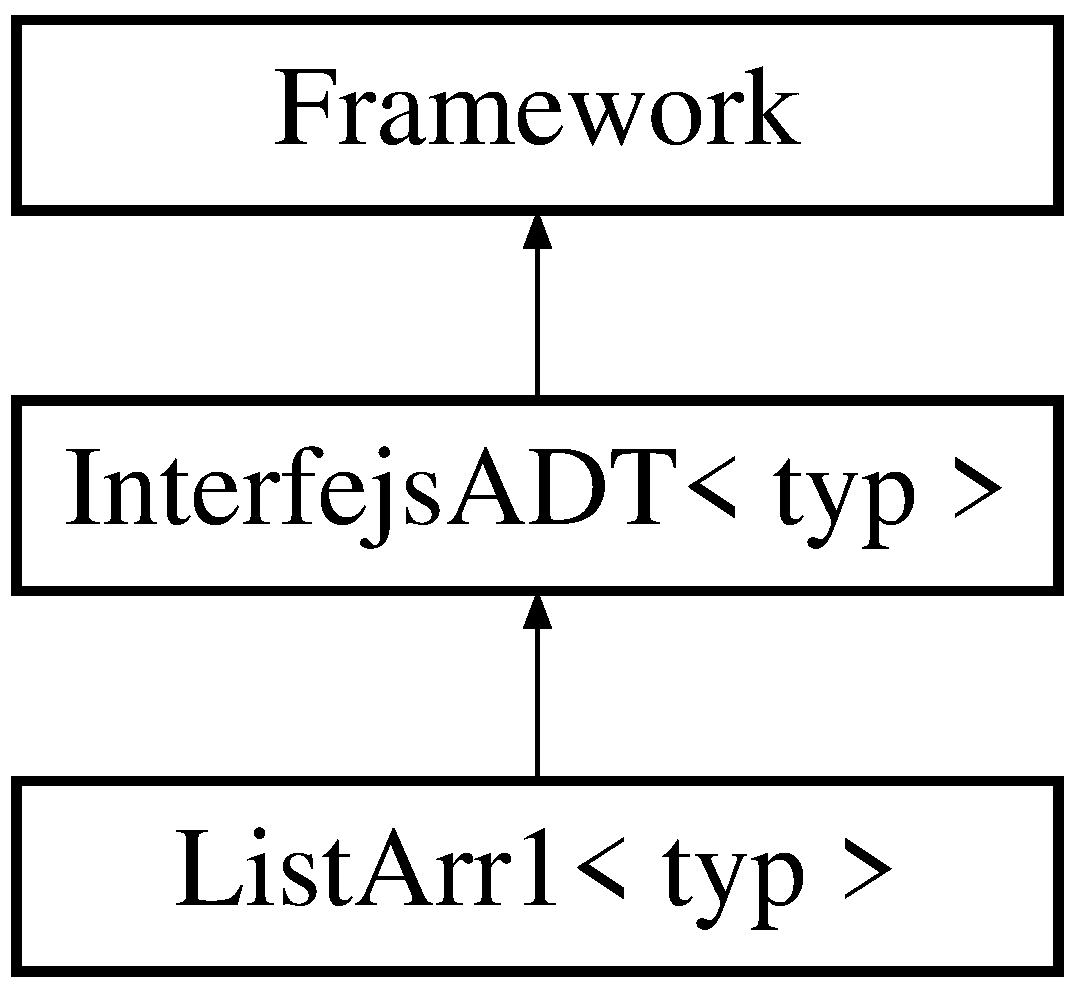
\includegraphics[height=3.000000cm]{class_list_arr1}
\end{center}
\end{figure}
\subsubsection*{Public Member Functions}
\begin{DoxyCompactItemize}
\item 
\hyperlink{class_list_arr1_adb0efe7b437d19a3cc7325b379f573bb}{List\-Arr1} ()
\begin{DoxyCompactList}\small\item\em Konstruktor bezarumentowy. \end{DoxyCompactList}\item 
void \hyperlink{class_list_arr1_a9b8bfbeae4e0b93ab47398d0282447b5}{push} (typ dana, unsigned int pole)
\begin{DoxyCompactList}\small\item\em Dodaje element do Listy\-Arr1. \end{DoxyCompactList}\item 
typ \hyperlink{class_list_arr1_acbc2f02d8ee4389cfd202beeddfae82c}{pop} (unsigned int pole)
\begin{DoxyCompactList}\small\item\em Pobiera element z Listy\-Arr1. \end{DoxyCompactList}\item 
unsigned int \hyperlink{class_list_arr1_a42b97b706c07e85f866bafd6ebc9b440}{size} ()
\begin{DoxyCompactList}\small\item\em Wielkość listy. \end{DoxyCompactList}\item 
void \hyperlink{class_list_arr1_a3af86b6f1d64d7a818faa726b83eb7e2}{Start} (const unsigned int k)
\begin{DoxyCompactList}\small\item\em Metoda testująca czas. \end{DoxyCompactList}\item 
void \hyperlink{class_list_arr1_a0a059d167f26e2498f3f4827f81841da}{Wczytaj\-Dane} (const char $\ast$nazwa\-Pliku, unsigned int n)
\begin{DoxyCompactList}\small\item\em Wczytuje dane z pliku. \end{DoxyCompactList}\item 
void \hyperlink{class_list_arr1_a613d2338847bd5d3b1383892d74280e7}{Zwolnij} ()
\begin{DoxyCompactList}\small\item\em Zwalnia pamięć \end{DoxyCompactList}\end{DoxyCompactItemize}
\subsubsection*{Private Attributes}
\begin{DoxyCompactItemize}
\item 
typ $\ast$ \hyperlink{class_list_arr1_ad411362d4d7884f0bbf5e081de7f2c6b}{tab}
\begin{DoxyCompactList}\small\item\em Wkaźnik na dynamiczną tablicę \end{DoxyCompactList}\item 
unsigned int \hyperlink{class_list_arr1_a1f1091116cd72de9affe8d4bcb1998a5}{Rozmiar\-T}
\begin{DoxyCompactList}\small\item\em Rozmiar tablicy. \end{DoxyCompactList}\item 
unsigned int \hyperlink{class_list_arr1_a08eada9ef97462cfa3906c5c8c1bc851}{Rozmiar\-L}
\begin{DoxyCompactList}\small\item\em Rozmiar Listy. \end{DoxyCompactList}\end{DoxyCompactItemize}


\subsubsection{Detailed Description}
\subsubsection*{template$<$class typ$>$class List\-Arr1$<$ typ $>$}

Modeluje pojęcie Listy (array) 

Modeluje pojęcie Listy opartej na dynamicznej tablicy. Dodając elementy zwiększa tablicę o 1. 

Definition at line 20 of file List\-Arr1.\-hh.



\subsubsection{Constructor \& Destructor Documentation}
\hypertarget{class_list_arr1_adb0efe7b437d19a3cc7325b379f573bb}{\index{List\-Arr1@{List\-Arr1}!List\-Arr1@{List\-Arr1}}
\index{List\-Arr1@{List\-Arr1}!ListArr1@{List\-Arr1}}
\paragraph[{List\-Arr1}]{\setlength{\rightskip}{0pt plus 5cm}template$<$class typ $>$ {\bf List\-Arr1}$<$ typ $>$\-::{\bf List\-Arr1} (
\begin{DoxyParamCaption}
{}
\end{DoxyParamCaption}
)\hspace{0.3cm}{\ttfamily [inline]}}}\label{class_list_arr1_adb0efe7b437d19a3cc7325b379f573bb}


Konstruktor bezarumentowy. 

Kontruktor alokujący tablicę jednoelementową z której będzie tworzona lista 

Definition at line 55 of file List\-Arr1.\-hh.



\subsubsection{Member Function Documentation}
\hypertarget{class_list_arr1_acbc2f02d8ee4389cfd202beeddfae82c}{\index{List\-Arr1@{List\-Arr1}!pop@{pop}}
\index{pop@{pop}!ListArr1@{List\-Arr1}}
\paragraph[{pop}]{\setlength{\rightskip}{0pt plus 5cm}template$<$class typ $>$ typ {\bf List\-Arr1}$<$ typ $>$\-::pop (
\begin{DoxyParamCaption}
\item[{unsigned int}]{pole}
\end{DoxyParamCaption}
)\hspace{0.3cm}{\ttfamily [inline]}, {\ttfamily [virtual]}}}\label{class_list_arr1_acbc2f02d8ee4389cfd202beeddfae82c}


Pobiera element z Listy\-Arr1. 

Pobiera element z Listy Arr1 usuwając go z niej i zmniejszając rozmiar.

param\mbox{[}in\mbox{]} -\/ pole -\/ nr pola z którgo chcemy pobrać element

retval -\/ zwraca wartosc pobranej danej lub '-\/1' w przyadku bledu 

Implements \hyperlink{class_interfejs_a_d_t_aa5a81a01c32577d986320524bcd091f0}{Interfejs\-A\-D\-T$<$ typ $>$}.



Definition at line 104 of file List\-Arr1.\-hh.

\hypertarget{class_list_arr1_a9b8bfbeae4e0b93ab47398d0282447b5}{\index{List\-Arr1@{List\-Arr1}!push@{push}}
\index{push@{push}!ListArr1@{List\-Arr1}}
\paragraph[{push}]{\setlength{\rightskip}{0pt plus 5cm}template$<$class typ $>$ void {\bf List\-Arr1}$<$ typ $>$\-::push (
\begin{DoxyParamCaption}
\item[{typ}]{dana, }
\item[{unsigned int}]{pole}
\end{DoxyParamCaption}
)\hspace{0.3cm}{\ttfamily [inline]}, {\ttfamily [virtual]}}}\label{class_list_arr1_a9b8bfbeae4e0b93ab47398d0282447b5}


Dodaje element do Listy\-Arr1. 

Dodaje nowy element do Listy\-Arr1


\begin{DoxyParams}[1]{Parameters}
\mbox{\tt in}  & {\em dana} & -\/ element który chcemy umieścić na liście \\
\hline
\mbox{\tt in}  & {\em pole} & -\/ nr pola na którym chcemy umieścić element jeżeli chcesz umieścić na początku listy podaj wartość 0, na końcu warość \hyperlink{class_list_arr1_a42b97b706c07e85f866bafd6ebc9b440}{size()} \\
\hline
\end{DoxyParams}


Implements \hyperlink{class_interfejs_a_d_t_abae6ef55c501edc4ca4e0faf4436b0df}{Interfejs\-A\-D\-T$<$ typ $>$}.



Definition at line 72 of file List\-Arr1.\-hh.

\hypertarget{class_list_arr1_a42b97b706c07e85f866bafd6ebc9b440}{\index{List\-Arr1@{List\-Arr1}!size@{size}}
\index{size@{size}!ListArr1@{List\-Arr1}}
\paragraph[{size}]{\setlength{\rightskip}{0pt plus 5cm}template$<$class typ $>$ unsigned int {\bf List\-Arr1}$<$ typ $>$\-::size (
\begin{DoxyParamCaption}
{}
\end{DoxyParamCaption}
)\hspace{0.3cm}{\ttfamily [inline]}, {\ttfamily [virtual]}}}\label{class_list_arr1_a42b97b706c07e85f866bafd6ebc9b440}


Wielkość listy. 

Informuje o ilości elementów znajdujących się na Liście\-Arr1


\begin{DoxyRetVals}{Return values}
{\em -\/} & zwraca liczbę elementów Listy\-Arr1 \\
\hline
\end{DoxyRetVals}


Implements \hyperlink{class_interfejs_a_d_t_a871cc26c895ce229ad04f7897fe4ba48}{Interfejs\-A\-D\-T$<$ typ $>$}.



Definition at line 137 of file List\-Arr1.\-hh.

\hypertarget{class_list_arr1_a3af86b6f1d64d7a818faa726b83eb7e2}{\index{List\-Arr1@{List\-Arr1}!Start@{Start}}
\index{Start@{Start}!ListArr1@{List\-Arr1}}
\paragraph[{Start}]{\setlength{\rightskip}{0pt plus 5cm}template$<$class typ $>$ void {\bf List\-Arr1}$<$ typ $>$\-::Start (
\begin{DoxyParamCaption}
\item[{const unsigned int}]{k}
\end{DoxyParamCaption}
)\hspace{0.3cm}{\ttfamily [inline]}}}\label{class_list_arr1_a3af86b6f1d64d7a818faa726b83eb7e2}


Metoda testująca czas. 

Metoda testująca czas wczytania n elementów na Listę\-Arr1


\begin{DoxyParams}[1]{Parameters}
\mbox{\tt in}  & {\em k} & -\/ ilość elementów do wczytania \\
\hline
\end{DoxyParams}


Definition at line 147 of file List\-Arr1.\-hh.

\hypertarget{class_list_arr1_a0a059d167f26e2498f3f4827f81841da}{\index{List\-Arr1@{List\-Arr1}!Wczytaj\-Dane@{Wczytaj\-Dane}}
\index{Wczytaj\-Dane@{Wczytaj\-Dane}!ListArr1@{List\-Arr1}}
\paragraph[{Wczytaj\-Dane}]{\setlength{\rightskip}{0pt plus 5cm}template$<$class typ $>$ void {\bf List\-Arr1}$<$ typ $>$\-::Wczytaj\-Dane (
\begin{DoxyParamCaption}
\item[{const char $\ast$}]{nazwa\-Pliku, }
\item[{unsigned int}]{n}
\end{DoxyParamCaption}
)\hspace{0.3cm}{\ttfamily [inline]}}}\label{class_list_arr1_a0a059d167f26e2498f3f4827f81841da}


Wczytuje dane z pliku. 

Wczytuje dane z pliku do \hyperlink{class_list_arr1}{List\-Arr1}

param\mbox{[}in\mbox{]} nazwa\-Pliku -\/ nazwa pliku z danymi param\mbox{[}in\mbox{]} n -\/ ilość danych do wczytania, 0 oznacza wszystkie dane z pliku 

Definition at line 161 of file List\-Arr1.\-hh.

\hypertarget{class_list_arr1_a613d2338847bd5d3b1383892d74280e7}{\index{List\-Arr1@{List\-Arr1}!Zwolnij@{Zwolnij}}
\index{Zwolnij@{Zwolnij}!ListArr1@{List\-Arr1}}
\paragraph[{Zwolnij}]{\setlength{\rightskip}{0pt plus 5cm}template$<$class typ $>$ void {\bf List\-Arr1}$<$ typ $>$\-::Zwolnij (
\begin{DoxyParamCaption}
{}
\end{DoxyParamCaption}
)\hspace{0.3cm}{\ttfamily [inline]}, {\ttfamily [virtual]}}}\label{class_list_arr1_a613d2338847bd5d3b1383892d74280e7}


Zwalnia pamięć 

Zwalnia pamięć zaalokowaną przez \hyperlink{class_list_arr1}{List\-Arr1} 

Implements \hyperlink{class_interfejs_a_d_t_a75427479b00e3d4a0c5f9615216262ea}{Interfejs\-A\-D\-T$<$ typ $>$}.



Definition at line 169 of file List\-Arr1.\-hh.



\subsubsection{Member Data Documentation}
\hypertarget{class_list_arr1_a08eada9ef97462cfa3906c5c8c1bc851}{\index{List\-Arr1@{List\-Arr1}!Rozmiar\-L@{Rozmiar\-L}}
\index{Rozmiar\-L@{Rozmiar\-L}!ListArr1@{List\-Arr1}}
\paragraph[{Rozmiar\-L}]{\setlength{\rightskip}{0pt plus 5cm}template$<$class typ $>$ unsigned int {\bf List\-Arr1}$<$ typ $>$\-::Rozmiar\-L\hspace{0.3cm}{\ttfamily [private]}}}\label{class_list_arr1_a08eada9ef97462cfa3906c5c8c1bc851}


Rozmiar Listy. 

Aktualny rozmiar Listy\-Arr1 

Definition at line 44 of file List\-Arr1.\-hh.

\hypertarget{class_list_arr1_a1f1091116cd72de9affe8d4bcb1998a5}{\index{List\-Arr1@{List\-Arr1}!Rozmiar\-T@{Rozmiar\-T}}
\index{Rozmiar\-T@{Rozmiar\-T}!ListArr1@{List\-Arr1}}
\paragraph[{Rozmiar\-T}]{\setlength{\rightskip}{0pt plus 5cm}template$<$class typ $>$ unsigned int {\bf List\-Arr1}$<$ typ $>$\-::Rozmiar\-T\hspace{0.3cm}{\ttfamily [private]}}}\label{class_list_arr1_a1f1091116cd72de9affe8d4bcb1998a5}


Rozmiar tablicy. 

Aktualny rozmiar tablicy. 

Definition at line 36 of file List\-Arr1.\-hh.

\hypertarget{class_list_arr1_ad411362d4d7884f0bbf5e081de7f2c6b}{\index{List\-Arr1@{List\-Arr1}!tab@{tab}}
\index{tab@{tab}!ListArr1@{List\-Arr1}}
\paragraph[{tab}]{\setlength{\rightskip}{0pt plus 5cm}template$<$class typ $>$ typ$\ast$ {\bf List\-Arr1}$<$ typ $>$\-::tab\hspace{0.3cm}{\ttfamily [private]}}}\label{class_list_arr1_ad411362d4d7884f0bbf5e081de7f2c6b}


Wkaźnik na dynamiczną tablicę 

Wskaźnik na dynamiczną tablicę tworzącą Listę\-Arr1 

Definition at line 28 of file List\-Arr1.\-hh.



The documentation for this class was generated from the following file\-:\begin{DoxyCompactItemize}
\item 
/home/bartolomeo/209296/prj/inc/\hyperlink{_list_arr1_8hh}{List\-Arr1.\-hh}\end{DoxyCompactItemize}

\hypertarget{class_list_arr2x}{\subsection{List\-Arr2x$<$ typ $>$ Class Template Reference}
\label{class_list_arr2x}\index{List\-Arr2x$<$ typ $>$@{List\-Arr2x$<$ typ $>$}}
}


Modeluje pojęcie Listy (array)  




{\ttfamily \#include $<$List\-Arr2x.\-hh$>$}

Inheritance diagram for List\-Arr2x$<$ typ $>$\-:\begin{figure}[H]
\begin{center}
\leavevmode
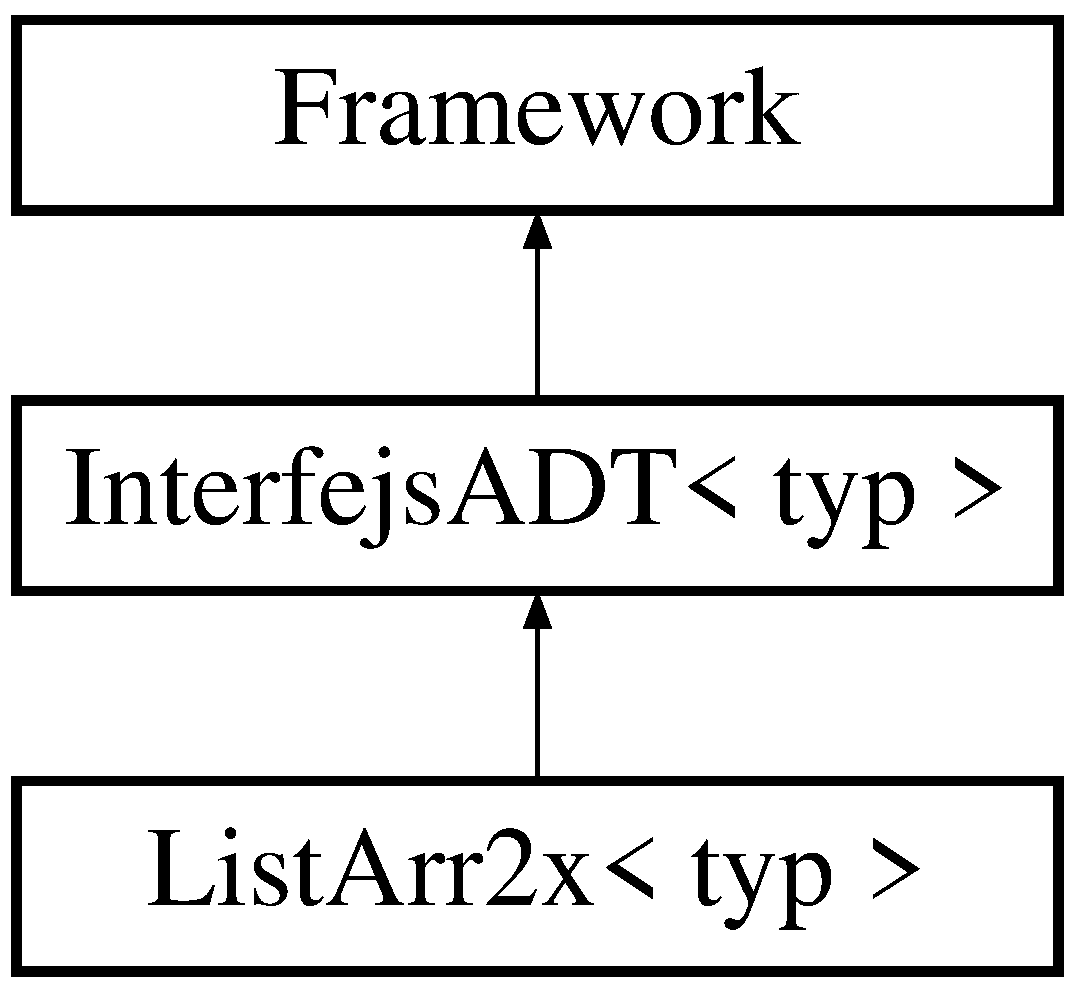
\includegraphics[height=3.000000cm]{class_list_arr2x}
\end{center}
\end{figure}
\subsubsection*{Public Member Functions}
\begin{DoxyCompactItemize}
\item 
\hyperlink{class_list_arr2x_abcda8405dca802e050c32cadb56f2caf}{List\-Arr2x} ()
\begin{DoxyCompactList}\small\item\em Konstruktor bezarumentowy. \end{DoxyCompactList}\item 
void \hyperlink{class_list_arr2x_a6aa004e56bdaf72de719d682b4069011}{push} (typ dana, unsigned int pole)
\begin{DoxyCompactList}\small\item\em Dodaje element do Listy\-Arr1. \end{DoxyCompactList}\item 
typ \hyperlink{class_list_arr2x_a6462ac1f547b7a090e54629539ce2dda}{pop} (unsigned int pole)
\begin{DoxyCompactList}\small\item\em Pobiera element z Listy\-Arr1. \end{DoxyCompactList}\item 
unsigned int \hyperlink{class_list_arr2x_a6097d85211e74053506d4a5dce86f26c}{size} ()
\begin{DoxyCompactList}\small\item\em Wielkość listy. \end{DoxyCompactList}\item 
void \hyperlink{class_list_arr2x_afd6469fa733da21b70981fa4dfae9c12}{Wczytaj\-Dane} (const std\-::string Plik\-In, unsigned int n)
\begin{DoxyCompactList}\small\item\em Wczytuje dane z pliku. \end{DoxyCompactList}\item 
void \hyperlink{class_list_arr2x_a7145b66ae33801053dc15bad1baa3085}{Qsort} (int l, int h)
\begin{DoxyCompactList}\small\item\em Metoda wykorzystujaca sortowanei szybkie. \end{DoxyCompactList}\item 
void \hyperlink{class_list_arr2x_a0c4ff2329317ccd77e48cf2965c80d91}{Qsort\-Opt} (int lewy, int prawy1)
\begin{DoxyCompactList}\small\item\em Zotymalizowane Sortowanie Szybkie. \end{DoxyCompactList}\item 
void \hyperlink{class_list_arr2x_a5f2644455c4c3a1ee9f1752a74857241}{Pokaz} ()
\begin{DoxyCompactList}\small\item\em Metoda wypisujaca elemeny listy. \end{DoxyCompactList}\item 
void \hyperlink{class_list_arr2x_a68dc47d3f73dbe42364bf34bdb132d00}{M\-Sort} (typ $\ast$T, int p, int k)
\end{DoxyCompactItemize}
\subsubsection*{Private Member Functions}
\begin{DoxyCompactItemize}
\item 
void \hyperlink{class_list_arr2x_abc4a5c934e4b30542f71045ec94c176b}{Wstaw\-\_\-\-Sort} (typ $\ast$T, int n)
\begin{DoxyCompactList}\small\item\em Sortowanie przez Wstawianie Metoda ma za zadanie posortowac tablice przyjmowana jako argument. \end{DoxyCompactList}\item 
int \hyperlink{class_list_arr2x_a8f0e72633b7bb63a37faaa99282b5308}{Mediana} (typ $\ast$W)
\begin{DoxyCompactList}\small\item\em Mediana Metoda wyznaczajaca mediana dla tablicy 3 elementowej. Jest to metoda pomocnicza, wykorzystywana przy optymalizacji doboru pivotu w sortowaniu szybkim. \end{DoxyCompactList}\item 
void \hyperlink{class_list_arr2x_adfd1dd69dadd19ac04ede03dba454fb5}{Start\-Msort} (unsigned int k)
\begin{DoxyCompactList}\small\item\em Metoda testująca czas. \end{DoxyCompactList}\item 
void \hyperlink{class_list_arr2x_ad73276a597d78b636119378ee408129d}{Start} ()
\begin{DoxyCompactList}\small\item\em Metoda testująca czas. \end{DoxyCompactList}\item 
void \hyperlink{class_list_arr2x_a8641af35d8316a58610a1c02ff4c3f83}{Zamien} (typ \&i, typ \&j)
\begin{DoxyCompactList}\small\item\em Metoda zamieniajaca Metoda ma za zadanie zamienic miejscami elementy wybrane przez argumenty wywolania. \end{DoxyCompactList}\item 
int \hyperlink{class_list_arr2x_a522da82666b97c2810ff458ef14e0996}{Partycjowanie} (int p, int k)
\begin{DoxyCompactList}\small\item\em Metoda segregujaca. \end{DoxyCompactList}\item 
void \hyperlink{class_list_arr2x_afcf6d8447657ff792afd631c54a4ff99}{Merge} (typ $\ast$Temp, int l, int s, int p)
\begin{DoxyCompactList}\small\item\em Metoda Dzielaca tablice. \end{DoxyCompactList}\item 
void \hyperlink{class_list_arr2x_a4e922603e7ed26334ee19cbca3c5056d}{Zwolnij} ()
\begin{DoxyCompactList}\small\item\em Zwalnia pamięć \end{DoxyCompactList}\end{DoxyCompactItemize}
\subsubsection*{Private Attributes}
\begin{DoxyCompactItemize}
\item 
typ $\ast$ \hyperlink{class_list_arr2x_aea5c139721e078af30bdc3c46cf58841}{tab}
\begin{DoxyCompactList}\small\item\em Wkaźnik na dynamiczną tablicę \end{DoxyCompactList}\item 
unsigned int \hyperlink{class_list_arr2x_aa25f050acca08e308c9b508f3ed8c912}{Rozmiar\-T}
\begin{DoxyCompactList}\small\item\em Rozmiar tablicy. \end{DoxyCompactList}\item 
unsigned int \hyperlink{class_list_arr2x_a17e0dfc0e9c86d433e0a79994af926c9}{Rozmiar\-L}
\begin{DoxyCompactList}\small\item\em Rozmiar Listy. \end{DoxyCompactList}\end{DoxyCompactItemize}


\subsubsection{Detailed Description}
\subsubsection*{template$<$class typ$>$class List\-Arr2x$<$ typ $>$}

Modeluje pojęcie Listy (array) 

Modeluje pojęcie Listy opartej na dynamicznej tablicy. Dodając elementy zwiększa tablicę dwukrotnie, jeżeli brakuje miejsca. 

Definition at line 23 of file List\-Arr2x.\-hh.



\subsubsection{Constructor \& Destructor Documentation}
\hypertarget{class_list_arr2x_abcda8405dca802e050c32cadb56f2caf}{\index{List\-Arr2x@{List\-Arr2x}!List\-Arr2x@{List\-Arr2x}}
\index{List\-Arr2x@{List\-Arr2x}!ListArr2x@{List\-Arr2x}}
\paragraph[{List\-Arr2x}]{\setlength{\rightskip}{0pt plus 5cm}template$<$class typ$>$ {\bf List\-Arr2x}$<$ typ $>$\-::{\bf List\-Arr2x} (
\begin{DoxyParamCaption}
{}
\end{DoxyParamCaption}
)\hspace{0.3cm}{\ttfamily [inline]}}}\label{class_list_arr2x_abcda8405dca802e050c32cadb56f2caf}


Konstruktor bezarumentowy. 

Kontruktor alokujący tablicę jednoelementową z której będzie tworzona lista 

Definition at line 222 of file List\-Arr2x.\-hh.



\subsubsection{Member Function Documentation}
\hypertarget{class_list_arr2x_a8f0e72633b7bb63a37faaa99282b5308}{\index{List\-Arr2x@{List\-Arr2x}!Mediana@{Mediana}}
\index{Mediana@{Mediana}!ListArr2x@{List\-Arr2x}}
\paragraph[{Mediana}]{\setlength{\rightskip}{0pt plus 5cm}template$<$class typ$>$ int {\bf List\-Arr2x}$<$ typ $>$\-::Mediana (
\begin{DoxyParamCaption}
\item[{typ $\ast$}]{W}
\end{DoxyParamCaption}
)\hspace{0.3cm}{\ttfamily [inline]}, {\ttfamily [private]}}}\label{class_list_arr2x_a8f0e72633b7bb63a37faaa99282b5308}


Mediana Metoda wyznaczajaca mediana dla tablicy 3 elementowej. Jest to metoda pomocnicza, wykorzystywana przy optymalizacji doboru pivotu w sortowaniu szybkim. 

\begin{DoxyReturn}{Returns}
Zwraca indeks na ktorym znajduje sie mediana w tablicy wejsciowej 
\end{DoxyReturn}


Definition at line 84 of file List\-Arr2x.\-hh.

\hypertarget{class_list_arr2x_afcf6d8447657ff792afd631c54a4ff99}{\index{List\-Arr2x@{List\-Arr2x}!Merge@{Merge}}
\index{Merge@{Merge}!ListArr2x@{List\-Arr2x}}
\paragraph[{Merge}]{\setlength{\rightskip}{0pt plus 5cm}template$<$class typ$>$ void {\bf List\-Arr2x}$<$ typ $>$\-::Merge (
\begin{DoxyParamCaption}
\item[{typ $\ast$}]{Temp, }
\item[{int}]{l, }
\item[{int}]{s, }
\item[{int}]{p}
\end{DoxyParamCaption}
)\hspace{0.3cm}{\ttfamily [inline]}, {\ttfamily [private]}}}\label{class_list_arr2x_afcf6d8447657ff792afd631c54a4ff99}


Metoda Dzielaca tablice. 

Metoda ma za zadanie przekopiowac zawartosc zbiotu glownego do tablicy tymczasowej.\-Nastepnie operujac na kopii ustawia wskazniki na poczatki kolejnych zbiorow i porownywane sa wskaane wartosci. Mniejsze wpisujemy do zbioru glownego i przesuwamy odpowiedni wskaznik Czynnos wykonujemy rekurencyjnie az do momentu gdy jeden ze wskaznikow osiagnie koniec zbioru


\begin{DoxyParams}[1]{Parameters}
\mbox{\tt in}  & {\em Temp} & -\/ Wskaznik na tablice pomocnicza \\
\hline
\mbox{\tt in}  & {\em l} & -\/ Poczatkowy indeks tablicy \\
\hline
\mbox{\tt in}  & {\em s} & -\/ Srodkowy indeks tablicy \\
\hline
\mbox{\tt in}  & {\em p} & -\/ Koncowy indks tablicy \\
\hline
\end{DoxyParams}


Definition at line 180 of file List\-Arr2x.\-hh.

\hypertarget{class_list_arr2x_a68dc47d3f73dbe42364bf34bdb132d00}{\index{List\-Arr2x@{List\-Arr2x}!M\-Sort@{M\-Sort}}
\index{M\-Sort@{M\-Sort}!ListArr2x@{List\-Arr2x}}
\paragraph[{M\-Sort}]{\setlength{\rightskip}{0pt plus 5cm}template$<$class typ$>$ void {\bf List\-Arr2x}$<$ typ $>$\-::M\-Sort (
\begin{DoxyParamCaption}
\item[{typ $\ast$}]{T, }
\item[{int}]{p, }
\item[{int}]{k}
\end{DoxyParamCaption}
)\hspace{0.3cm}{\ttfamily [inline]}}}\label{class_list_arr2x_a68dc47d3f73dbe42364bf34bdb132d00}


Definition at line 449 of file List\-Arr2x.\-hh.

\hypertarget{class_list_arr2x_a522da82666b97c2810ff458ef14e0996}{\index{List\-Arr2x@{List\-Arr2x}!Partycjowanie@{Partycjowanie}}
\index{Partycjowanie@{Partycjowanie}!ListArr2x@{List\-Arr2x}}
\paragraph[{Partycjowanie}]{\setlength{\rightskip}{0pt plus 5cm}template$<$class typ$>$ int {\bf List\-Arr2x}$<$ typ $>$\-::Partycjowanie (
\begin{DoxyParamCaption}
\item[{int}]{p, }
\item[{int}]{k}
\end{DoxyParamCaption}
)\hspace{0.3cm}{\ttfamily [inline]}, {\ttfamily [private]}}}\label{class_list_arr2x_a522da82666b97c2810ff458ef14e0996}


Metoda segregujaca. 

Metoda ma za zadanie wybor elementu, ktory ma byc uzyty do podzialu i przenosi wszytskie elementy mniejsze na lewo od tego elementu, a wieksze elementy na prawo od wybranego elementu 
\begin{DoxyParams}[1]{Parameters}
\mbox{\tt in}  & {\em p} & -\/ poczatkowy indeks podzbiotru \\
\hline
\mbox{\tt in}  & {\em k} & -\/ koncowy indeks podzbioru \\
\hline
\end{DoxyParams}
\begin{DoxyReturn}{Returns}

\end{DoxyReturn}


Definition at line 147 of file List\-Arr2x.\-hh.

\hypertarget{class_list_arr2x_a5f2644455c4c3a1ee9f1752a74857241}{\index{List\-Arr2x@{List\-Arr2x}!Pokaz@{Pokaz}}
\index{Pokaz@{Pokaz}!ListArr2x@{List\-Arr2x}}
\paragraph[{Pokaz}]{\setlength{\rightskip}{0pt plus 5cm}template$<$class typ$>$ void {\bf List\-Arr2x}$<$ typ $>$\-::Pokaz (
\begin{DoxyParamCaption}
{}
\end{DoxyParamCaption}
)\hspace{0.3cm}{\ttfamily [inline]}, {\ttfamily [virtual]}}}\label{class_list_arr2x_a5f2644455c4c3a1ee9f1752a74857241}


Metoda wypisujaca elemeny listy. 

Metoda ma za zadanie wypisac wszystkie elementy znajdujace sie obecnie na liscie danych 

Implements \hyperlink{class_interfejs_a_d_t_a22e091ad4cdcade33f9fa579a90ebf79}{Interfejs\-A\-D\-T$<$ typ $>$}.



Definition at line 439 of file List\-Arr2x.\-hh.

\hypertarget{class_list_arr2x_a6462ac1f547b7a090e54629539ce2dda}{\index{List\-Arr2x@{List\-Arr2x}!pop@{pop}}
\index{pop@{pop}!ListArr2x@{List\-Arr2x}}
\paragraph[{pop}]{\setlength{\rightskip}{0pt plus 5cm}template$<$class typ$>$ typ {\bf List\-Arr2x}$<$ typ $>$\-::pop (
\begin{DoxyParamCaption}
\item[{unsigned int}]{pole}
\end{DoxyParamCaption}
)\hspace{0.3cm}{\ttfamily [inline]}, {\ttfamily [virtual]}}}\label{class_list_arr2x_a6462ac1f547b7a090e54629539ce2dda}


Pobiera element z Listy\-Arr1. 

Pobiera element z Listy\-Arr2x usuwając go z niej i zmniejszając rozmiar o połowę w przypadku przekroczenia stosunku 1\-:4 (Rozmiar\-L\-:Rozmiar\-T)

param\mbox{[}in\mbox{]} -\/ pole -\/ nr pola z którgo chcemy pobrać element (indeksowane od 0)

retval -\/ zwraca wartosc pobranej danej lub '-\/1' w przyadku bledu 

Implements \hyperlink{class_interfejs_a_d_t_aa5a81a01c32577d986320524bcd091f0}{Interfejs\-A\-D\-T$<$ typ $>$}.



Definition at line 293 of file List\-Arr2x.\-hh.

\hypertarget{class_list_arr2x_a6aa004e56bdaf72de719d682b4069011}{\index{List\-Arr2x@{List\-Arr2x}!push@{push}}
\index{push@{push}!ListArr2x@{List\-Arr2x}}
\paragraph[{push}]{\setlength{\rightskip}{0pt plus 5cm}template$<$class typ$>$ void {\bf List\-Arr2x}$<$ typ $>$\-::push (
\begin{DoxyParamCaption}
\item[{typ}]{dana, }
\item[{unsigned int}]{pole}
\end{DoxyParamCaption}
)\hspace{0.3cm}{\ttfamily [inline]}, {\ttfamily [virtual]}}}\label{class_list_arr2x_a6aa004e56bdaf72de719d682b4069011}


Dodaje element do Listy\-Arr1. 

Dodaje nowy element do Listy\-Arr1


\begin{DoxyParams}[1]{Parameters}
\mbox{\tt in}  & {\em dana} & -\/ element który chcemy umieścić na liście \\
\hline
\mbox{\tt in}  & {\em pole} & -\/ nr pola na którym chcemy umieścić element jeżeli chcesz umieścić na początku listy podaj wartość 0, na końcu warość \hyperlink{class_list_arr2x_a6097d85211e74053506d4a5dce86f26c}{size()} \\
\hline
\end{DoxyParams}


Implements \hyperlink{class_interfejs_a_d_t_abae6ef55c501edc4ca4e0faf4436b0df}{Interfejs\-A\-D\-T$<$ typ $>$}.



Definition at line 240 of file List\-Arr2x.\-hh.

\hypertarget{class_list_arr2x_a7145b66ae33801053dc15bad1baa3085}{\index{List\-Arr2x@{List\-Arr2x}!Qsort@{Qsort}}
\index{Qsort@{Qsort}!ListArr2x@{List\-Arr2x}}
\paragraph[{Qsort}]{\setlength{\rightskip}{0pt plus 5cm}template$<$class typ$>$ void {\bf List\-Arr2x}$<$ typ $>$\-::Qsort (
\begin{DoxyParamCaption}
\item[{int}]{l, }
\item[{int}]{h}
\end{DoxyParamCaption}
)\hspace{0.3cm}{\ttfamily [inline]}}}\label{class_list_arr2x_a7145b66ae33801053dc15bad1baa3085}


Metoda wykorzystujaca sortowanei szybkie. 


\begin{DoxyParams}[1]{Parameters}
\mbox{\tt in}  & {\em l} & -\/ poczatkowy indeks tablicy \\
\hline
\mbox{\tt in}  & {\em h} & -\/ koncowy indeks tablicy \\
\hline
\end{DoxyParams}


Definition at line 389 of file List\-Arr2x.\-hh.

\hypertarget{class_list_arr2x_a0c4ff2329317ccd77e48cf2965c80d91}{\index{List\-Arr2x@{List\-Arr2x}!Qsort\-Opt@{Qsort\-Opt}}
\index{Qsort\-Opt@{Qsort\-Opt}!ListArr2x@{List\-Arr2x}}
\paragraph[{Qsort\-Opt}]{\setlength{\rightskip}{0pt plus 5cm}template$<$class typ$>$ void {\bf List\-Arr2x}$<$ typ $>$\-::Qsort\-Opt (
\begin{DoxyParamCaption}
\item[{int}]{lewy, }
\item[{int}]{prawy1}
\end{DoxyParamCaption}
)\hspace{0.3cm}{\ttfamily [inline]}}}\label{class_list_arr2x_a0c4ff2329317ccd77e48cf2965c80d91}


Zotymalizowane Sortowanie Szybkie. 

Metoda modeluje algorytm sorotwanie szybkiego z zaimplementowanym algorytmem doboru pivotu, tak aby nie zostal wybrany najmniejszy element w danym podzbiorze. \mbox{[}in\mbox{]} lewy -\/poczatkowy indeks pozbioru 
\begin{DoxyParams}[1]{Parameters}
\mbox{\tt in}  & {\em prawy} & -\/ koncowy indeks podzbioru \\
\hline
\end{DoxyParams}


Definition at line 410 of file List\-Arr2x.\-hh.

\hypertarget{class_list_arr2x_a6097d85211e74053506d4a5dce86f26c}{\index{List\-Arr2x@{List\-Arr2x}!size@{size}}
\index{size@{size}!ListArr2x@{List\-Arr2x}}
\paragraph[{size}]{\setlength{\rightskip}{0pt plus 5cm}template$<$class typ$>$ unsigned int {\bf List\-Arr2x}$<$ typ $>$\-::size (
\begin{DoxyParamCaption}
{}
\end{DoxyParamCaption}
)\hspace{0.3cm}{\ttfamily [inline]}, {\ttfamily [virtual]}}}\label{class_list_arr2x_a6097d85211e74053506d4a5dce86f26c}


Wielkość listy. 

Informuje o ilości elementów znajdujących się na Liście\-Arr1


\begin{DoxyRetVals}{Return values}
{\em -\/} & zwraca liczbę elementów Listy\-Arr1 \\
\hline
\end{DoxyRetVals}


Implements \hyperlink{class_interfejs_a_d_t_a871cc26c895ce229ad04f7897fe4ba48}{Interfejs\-A\-D\-T$<$ typ $>$}.



Definition at line 345 of file List\-Arr2x.\-hh.

\hypertarget{class_list_arr2x_ad73276a597d78b636119378ee408129d}{\index{List\-Arr2x@{List\-Arr2x}!Start@{Start}}
\index{Start@{Start}!ListArr2x@{List\-Arr2x}}
\paragraph[{Start}]{\setlength{\rightskip}{0pt plus 5cm}template$<$class typ$>$ void {\bf List\-Arr2x}$<$ typ $>$\-::Start (
\begin{DoxyParamCaption}
{}
\end{DoxyParamCaption}
)\hspace{0.3cm}{\ttfamily [inline]}, {\ttfamily [private]}, {\ttfamily [virtual]}}}\label{class_list_arr2x_ad73276a597d78b636119378ee408129d}


Metoda testująca czas. 

Metoda testująca czas wczytania n elementów na Listę\-Arr1 

Implements \hyperlink{class_interfejs_a_d_t_ae4f4f725bf09c5b258bc0d12e0f589d8}{Interfejs\-A\-D\-T$<$ typ $>$}.



Definition at line 117 of file List\-Arr2x.\-hh.

\hypertarget{class_list_arr2x_adfd1dd69dadd19ac04ede03dba454fb5}{\index{List\-Arr2x@{List\-Arr2x}!Start\-Msort@{Start\-Msort}}
\index{Start\-Msort@{Start\-Msort}!ListArr2x@{List\-Arr2x}}
\paragraph[{Start\-Msort}]{\setlength{\rightskip}{0pt plus 5cm}template$<$class typ$>$ void {\bf List\-Arr2x}$<$ typ $>$\-::Start\-Msort (
\begin{DoxyParamCaption}
\item[{unsigned int}]{k}
\end{DoxyParamCaption}
)\hspace{0.3cm}{\ttfamily [inline]}, {\ttfamily [private]}, {\ttfamily [virtual]}}}\label{class_list_arr2x_adfd1dd69dadd19ac04ede03dba454fb5}


Metoda testująca czas. 

Metoda testująca czas wczytania n elementów na Listę\-Arr1


\begin{DoxyParams}[1]{Parameters}
\mbox{\tt in}  & {\em k} & -\/ ilość elementów do wczytania \\
\hline
\end{DoxyParams}


Implements \hyperlink{class_interfejs_a_d_t_a7fc6b6c9b0606a24846b7e744ee8a823}{Interfejs\-A\-D\-T$<$ typ $>$}.



Definition at line 104 of file List\-Arr2x.\-hh.

\hypertarget{class_list_arr2x_afd6469fa733da21b70981fa4dfae9c12}{\index{List\-Arr2x@{List\-Arr2x}!Wczytaj\-Dane@{Wczytaj\-Dane}}
\index{Wczytaj\-Dane@{Wczytaj\-Dane}!ListArr2x@{List\-Arr2x}}
\paragraph[{Wczytaj\-Dane}]{\setlength{\rightskip}{0pt plus 5cm}template$<$class typ$>$ void {\bf List\-Arr2x}$<$ typ $>$\-::Wczytaj\-Dane (
\begin{DoxyParamCaption}
\item[{const std\-::string}]{Plik\-In, }
\item[{unsigned int}]{n}
\end{DoxyParamCaption}
)\hspace{0.3cm}{\ttfamily [inline]}, {\ttfamily [virtual]}}}\label{class_list_arr2x_afd6469fa733da21b70981fa4dfae9c12}


Wczytuje dane z pliku. 

Wczytuje dane z pliku do \hyperlink{class_list_arr1}{List\-Arr1}

param\mbox{[}in\mbox{]} nazwa\-Pliku -\/ nazwa pliku z danymi param\mbox{[}in\mbox{]} n -\/ ilość danych do wczytania, 0 oznacza wszystkie dane z pliku 

Implements \hyperlink{class_interfejs_a_d_t_ae37b5d3abf3a7a85adf02e42e09df875}{Interfejs\-A\-D\-T$<$ typ $>$}.



Definition at line 357 of file List\-Arr2x.\-hh.

\hypertarget{class_list_arr2x_abc4a5c934e4b30542f71045ec94c176b}{\index{List\-Arr2x@{List\-Arr2x}!Wstaw\-\_\-\-Sort@{Wstaw\-\_\-\-Sort}}
\index{Wstaw\-\_\-\-Sort@{Wstaw\-\_\-\-Sort}!ListArr2x@{List\-Arr2x}}
\paragraph[{Wstaw\-\_\-\-Sort}]{\setlength{\rightskip}{0pt plus 5cm}template$<$class typ$>$ void {\bf List\-Arr2x}$<$ typ $>$\-::Wstaw\-\_\-\-Sort (
\begin{DoxyParamCaption}
\item[{typ $\ast$}]{T, }
\item[{int}]{n}
\end{DoxyParamCaption}
)\hspace{0.3cm}{\ttfamily [inline]}, {\ttfamily [private]}}}\label{class_list_arr2x_abc4a5c934e4b30542f71045ec94c176b}


Sortowanie przez Wstawianie Metoda ma za zadanie posortowac tablice przyjmowana jako argument. 


\begin{DoxyParams}[1]{Parameters}
\mbox{\tt in}  & {\em T} & -\/ Wskaznik na tablice z danymi wejsciowymi \\
\hline
\mbox{\tt in}  & {\em n} & -\/ ilosc \\
\hline
\end{DoxyParams}


Definition at line 59 of file List\-Arr2x.\-hh.

\hypertarget{class_list_arr2x_a8641af35d8316a58610a1c02ff4c3f83}{\index{List\-Arr2x@{List\-Arr2x}!Zamien@{Zamien}}
\index{Zamien@{Zamien}!ListArr2x@{List\-Arr2x}}
\paragraph[{Zamien}]{\setlength{\rightskip}{0pt plus 5cm}template$<$class typ$>$ void {\bf List\-Arr2x}$<$ typ $>$\-::Zamien (
\begin{DoxyParamCaption}
\item[{typ \&}]{i, }
\item[{typ \&}]{j}
\end{DoxyParamCaption}
)\hspace{0.3cm}{\ttfamily [inline]}, {\ttfamily [private]}}}\label{class_list_arr2x_a8641af35d8316a58610a1c02ff4c3f83}


Metoda zamieniajaca Metoda ma za zadanie zamienic miejscami elementy wybrane przez argumenty wywolania. 


\begin{DoxyParams}[1]{Parameters}
\mbox{\tt in}  & {\em i} & -\/ Adres elementu podlegajacy zamianie \\
\hline
\mbox{\tt in}  & {\em j} & -\/ Adres elementu podlegajacy zamianie \\
\hline
\end{DoxyParams}


Definition at line 130 of file List\-Arr2x.\-hh.

\hypertarget{class_list_arr2x_a4e922603e7ed26334ee19cbca3c5056d}{\index{List\-Arr2x@{List\-Arr2x}!Zwolnij@{Zwolnij}}
\index{Zwolnij@{Zwolnij}!ListArr2x@{List\-Arr2x}}
\paragraph[{Zwolnij}]{\setlength{\rightskip}{0pt plus 5cm}template$<$class typ$>$ void {\bf List\-Arr2x}$<$ typ $>$\-::Zwolnij (
\begin{DoxyParamCaption}
{}
\end{DoxyParamCaption}
)\hspace{0.3cm}{\ttfamily [inline]}, {\ttfamily [private]}, {\ttfamily [virtual]}}}\label{class_list_arr2x_a4e922603e7ed26334ee19cbca3c5056d}


Zwalnia pamięć 

Zwalnia pamięć zaalokowaną przez \hyperlink{class_list_arr1}{List\-Arr1} 

Implements \hyperlink{class_interfejs_a_d_t_a75427479b00e3d4a0c5f9615216262ea}{Interfejs\-A\-D\-T$<$ typ $>$}.



Definition at line 201 of file List\-Arr2x.\-hh.



\subsubsection{Member Data Documentation}
\hypertarget{class_list_arr2x_a17e0dfc0e9c86d433e0a79994af926c9}{\index{List\-Arr2x@{List\-Arr2x}!Rozmiar\-L@{Rozmiar\-L}}
\index{Rozmiar\-L@{Rozmiar\-L}!ListArr2x@{List\-Arr2x}}
\paragraph[{Rozmiar\-L}]{\setlength{\rightskip}{0pt plus 5cm}template$<$class typ$>$ unsigned int {\bf List\-Arr2x}$<$ typ $>$\-::Rozmiar\-L\hspace{0.3cm}{\ttfamily [private]}}}\label{class_list_arr2x_a17e0dfc0e9c86d433e0a79994af926c9}


Rozmiar Listy. 

Aktualny rozmiar Listy\-Arr2x 

Definition at line 50 of file List\-Arr2x.\-hh.

\hypertarget{class_list_arr2x_aa25f050acca08e308c9b508f3ed8c912}{\index{List\-Arr2x@{List\-Arr2x}!Rozmiar\-T@{Rozmiar\-T}}
\index{Rozmiar\-T@{Rozmiar\-T}!ListArr2x@{List\-Arr2x}}
\paragraph[{Rozmiar\-T}]{\setlength{\rightskip}{0pt plus 5cm}template$<$class typ$>$ unsigned int {\bf List\-Arr2x}$<$ typ $>$\-::Rozmiar\-T\hspace{0.3cm}{\ttfamily [private]}}}\label{class_list_arr2x_aa25f050acca08e308c9b508f3ed8c912}


Rozmiar tablicy. 

Aktualny rozmiar tablicy. 

Definition at line 41 of file List\-Arr2x.\-hh.

\hypertarget{class_list_arr2x_aea5c139721e078af30bdc3c46cf58841}{\index{List\-Arr2x@{List\-Arr2x}!tab@{tab}}
\index{tab@{tab}!ListArr2x@{List\-Arr2x}}
\paragraph[{tab}]{\setlength{\rightskip}{0pt plus 5cm}template$<$class typ$>$ typ$\ast$ {\bf List\-Arr2x}$<$ typ $>$\-::tab\hspace{0.3cm}{\ttfamily [private]}}}\label{class_list_arr2x_aea5c139721e078af30bdc3c46cf58841}


Wkaźnik na dynamiczną tablicę 

Wskaźnik na dynamiczną tablicę tworzącą Listę\-Arr2x 

Definition at line 32 of file List\-Arr2x.\-hh.



The documentation for this class was generated from the following file\-:\begin{DoxyCompactItemize}
\item 
/home/bartolomeo/209296/prj/inc/\hyperlink{_list_arr2x_8hh}{List\-Arr2x.\-hh}\end{DoxyCompactItemize}

\hypertarget{class_statystyka}{\subsection{Statystyka Class Reference}
\label{class_statystyka}\index{Statystyka@{Statystyka}}
}


Modeluje pojęcie statystyki.  




{\ttfamily \#include $<$Statystyka.\-hh$>$}

\subsubsection*{Public Member Functions}
\begin{DoxyCompactItemize}
\item 
\hyperlink{class_statystyka_a93d6a8763a84859ac52ec222b5ce31a6}{Statystyka} (const unsigned int ilosc\-Prob, unsigned int $\ast$proby)
\begin{DoxyCompactList}\small\item\em Konstruktor z dwoma pramametrami. \end{DoxyCompactList}\item 
\hyperlink{class_statystyka_ab9e4be151572e6851af96c08812a602a}{$\sim$\-Statystyka} ()
\begin{DoxyCompactList}\small\item\em Destruktor -\/ zwaknia pamięć \end{DoxyCompactList}\item 
double \& \hyperlink{class_statystyka_a651fc79171891fdb793836c2d1ac4669}{operator\mbox{[}$\,$\mbox{]}} (unsigned int i)
\begin{DoxyCompactList}\small\item\em Indeksuje tablicę czasową \end{DoxyCompactList}\item 
void \hyperlink{class_statystyka_a922a015761e06edcb9ff966cd0af16ab}{Zapisz\-Staty} (std\-::string nazwa\-Pliku)
\begin{DoxyCompactList}\small\item\em Zapisuje statysykę do pliku. \end{DoxyCompactList}\end{DoxyCompactItemize}
\subsubsection*{Private Attributes}
\begin{DoxyCompactItemize}
\item 
unsigned int \hyperlink{class_statystyka_af8bf74c21adf05068de9f7a02431ff6f}{Ile\-Prob}
\begin{DoxyCompactList}\small\item\em Ilość prób. \end{DoxyCompactList}\item 
unsigned int $\ast$ \hyperlink{class_statystyka_a4a34deeb4851d6e1418ba4e8f427e003}{Proba}
\begin{DoxyCompactList}\small\item\em Tablica z rozmiarami prób. \end{DoxyCompactList}\item 
double $\ast$ \hyperlink{class_statystyka_a0746642eb84423a747c1f857661288e5}{Czas}
\begin{DoxyCompactList}\small\item\em Średni czas wykonania danej próby. \end{DoxyCompactList}\end{DoxyCompactItemize}


\subsubsection{Detailed Description}
Modeluje pojęcie statystyki. 

Modeluje pojęcie statystyki, czyli średnich czasów wykonania metody dla różnyuch wielkości prób. 

Definition at line 22 of file Statystyka.\-hh.



\subsubsection{Constructor \& Destructor Documentation}
\hypertarget{class_statystyka_a93d6a8763a84859ac52ec222b5ce31a6}{\index{Statystyka@{Statystyka}!Statystyka@{Statystyka}}
\index{Statystyka@{Statystyka}!Statystyka@{Statystyka}}
\paragraph[{Statystyka}]{\setlength{\rightskip}{0pt plus 5cm}Statystyka\-::\-Statystyka (
\begin{DoxyParamCaption}
\item[{const unsigned int}]{ilosc\-Prob, }
\item[{unsigned int $\ast$}]{proby}
\end{DoxyParamCaption}
)}}\label{class_statystyka_a93d6a8763a84859ac52ec222b5ce31a6}


Konstruktor z dwoma pramametrami. 

Konstruktor z dwoma paramatremi tworzy dynamiczne tablice przechowujące statystykę oraz wypełnia rozmiary prób.


\begin{DoxyParams}[1]{Parameters}
\mbox{\tt in}  & {\em ilosc\-Prob} & -\/ liczbosc prob w ksperymencie \\
\hline
\mbox{\tt in}  & {\em proby} & -\/ tablica z licznościami prób. \\
\hline
\end{DoxyParams}


Definition at line 14 of file Statystyka.\-cpp.

\hypertarget{class_statystyka_ab9e4be151572e6851af96c08812a602a}{\index{Statystyka@{Statystyka}!$\sim$\-Statystyka@{$\sim$\-Statystyka}}
\index{$\sim$\-Statystyka@{$\sim$\-Statystyka}!Statystyka@{Statystyka}}
\paragraph[{$\sim$\-Statystyka}]{\setlength{\rightskip}{0pt plus 5cm}Statystyka\-::$\sim$\-Statystyka (
\begin{DoxyParamCaption}
{}
\end{DoxyParamCaption}
)\hspace{0.3cm}{\ttfamily [inline]}}}\label{class_statystyka_ab9e4be151572e6851af96c08812a602a}


Destruktor -\/ zwaknia pamięć 

Zwalnia pamięć zaalokowaną na dynamiczne tablicy przechowujące statystykę. 

Definition at line 68 of file Statystyka.\-hh.



\subsubsection{Member Function Documentation}
\hypertarget{class_statystyka_a651fc79171891fdb793836c2d1ac4669}{\index{Statystyka@{Statystyka}!operator\mbox{[}$\,$\mbox{]}@{operator[]}}
\index{operator\mbox{[}$\,$\mbox{]}@{operator[]}!Statystyka@{Statystyka}}
\paragraph[{operator[]}]{\setlength{\rightskip}{0pt plus 5cm}double\& Statystyka\-::operator\mbox{[}$\,$\mbox{]} (
\begin{DoxyParamCaption}
\item[{unsigned int}]{i}
\end{DoxyParamCaption}
)\hspace{0.3cm}{\ttfamily [inline]}}}\label{class_statystyka_a651fc79171891fdb793836c2d1ac4669}


Indeksuje tablicę czasową 

Zwraca referencję do i-\/tego indeksu tablicy czasowej.


\begin{DoxyParams}[1]{Parameters}
\mbox{\tt in}  & {\em i} & -\/ indeks tablicy czasowej\\
\hline
\end{DoxyParams}

\begin{DoxyRetVals}{Return values}
{\em Czas\mbox{[}i\mbox{]}} & referencja do wybranego indeksu \\
\hline
\end{DoxyRetVals}


Definition at line 80 of file Statystyka.\-hh.

\hypertarget{class_statystyka_a922a015761e06edcb9ff966cd0af16ab}{\index{Statystyka@{Statystyka}!Zapisz\-Staty@{Zapisz\-Staty}}
\index{Zapisz\-Staty@{Zapisz\-Staty}!Statystyka@{Statystyka}}
\paragraph[{Zapisz\-Staty}]{\setlength{\rightskip}{0pt plus 5cm}void Statystyka\-::\-Zapisz\-Staty (
\begin{DoxyParamCaption}
\item[{std\-::string}]{nazwa\-Pliku}
\end{DoxyParamCaption}
)}}\label{class_statystyka_a922a015761e06edcb9ff966cd0af16ab}


Zapisuje statysykę do pliku. 

Zapisuje statystystykę do pliku o nazwie \char`\"{}statystyka.\-dat\char`\"{}. Pierwsza linia pliku to wielkości prób druga to średnie czasy wykonania podane w ms; 

Definition at line 22 of file Statystyka.\-cpp.



\subsubsection{Member Data Documentation}
\hypertarget{class_statystyka_a0746642eb84423a747c1f857661288e5}{\index{Statystyka@{Statystyka}!Czas@{Czas}}
\index{Czas@{Czas}!Statystyka@{Statystyka}}
\paragraph[{Czas}]{\setlength{\rightskip}{0pt plus 5cm}double$\ast$ Statystyka\-::\-Czas\hspace{0.3cm}{\ttfamily [private]}}}\label{class_statystyka_a0746642eb84423a747c1f857661288e5}


Średni czas wykonania danej próby. 

wskaźnik na tablica ze średnimi czasami wykonania kolejnych prób. 

Definition at line 46 of file Statystyka.\-hh.

\hypertarget{class_statystyka_af8bf74c21adf05068de9f7a02431ff6f}{\index{Statystyka@{Statystyka}!Ile\-Prob@{Ile\-Prob}}
\index{Ile\-Prob@{Ile\-Prob}!Statystyka@{Statystyka}}
\paragraph[{Ile\-Prob}]{\setlength{\rightskip}{0pt plus 5cm}unsigned int Statystyka\-::\-Ile\-Prob\hspace{0.3cm}{\ttfamily [private]}}}\label{class_statystyka_af8bf74c21adf05068de9f7a02431ff6f}


Ilość prób. 

Ilość prób do utworzenia statystyki 

Definition at line 30 of file Statystyka.\-hh.

\hypertarget{class_statystyka_a4a34deeb4851d6e1418ba4e8f427e003}{\index{Statystyka@{Statystyka}!Proba@{Proba}}
\index{Proba@{Proba}!Statystyka@{Statystyka}}
\paragraph[{Proba}]{\setlength{\rightskip}{0pt plus 5cm}unsigned int$\ast$ Statystyka\-::\-Proba\hspace{0.3cm}{\ttfamily [private]}}}\label{class_statystyka_a4a34deeb4851d6e1418ba4e8f427e003}


Tablica z rozmiarami prób. 

Wskaźnik na tablicę zawierającą wielkości danych prób. 

Definition at line 38 of file Statystyka.\-hh.



The documentation for this class was generated from the following files\-:\begin{DoxyCompactItemize}
\item 
/home/bartolomeo/209296/prj/inc/\hyperlink{_statystyka_8hh}{Statystyka.\-hh}\item 
/home/bartolomeo/209296/prj/src/\hyperlink{_statystyka_8cpp}{Statystyka.\-cpp}\end{DoxyCompactItemize}

\hypertarget{class_stos}{\subsection{Stos$<$ typ $>$ Class Template Reference}
\label{class_stos}\index{Stos$<$ typ $>$@{Stos$<$ typ $>$}}
}


Modeluje pojęcie Stosu.  




{\ttfamily \#include $<$Stos.\-hh$>$}

Inheritance diagram for Stos$<$ typ $>$\-:\begin{figure}[H]
\begin{center}
\leavevmode
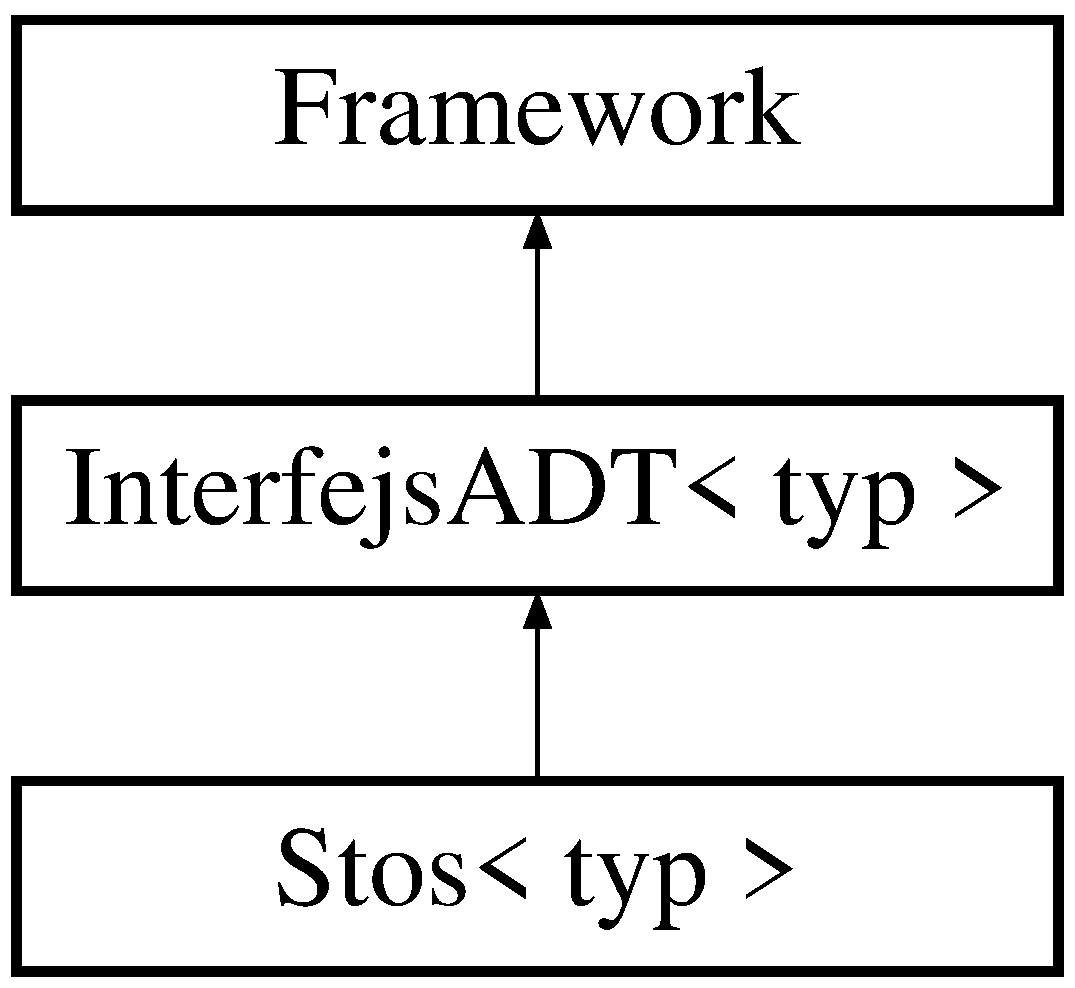
\includegraphics[height=3.000000cm]{class_stos}
\end{center}
\end{figure}
\subsubsection*{Classes}
\begin{DoxyCompactItemize}
\item 
struct \hyperlink{struct_stos_1_1_element}{Element}
\begin{DoxyCompactList}\small\item\em Modeluje jeden element Stosu. \end{DoxyCompactList}\end{DoxyCompactItemize}
\subsubsection*{Public Member Functions}
\begin{DoxyCompactItemize}
\item 
\hyperlink{class_stos_afc525fb8a9f8f80fda9bf0f846c078c4}{Stos} ()
\begin{DoxyCompactList}\small\item\em Konstruktor pustego Stosu. \end{DoxyCompactList}\item 
void \hyperlink{class_stos_a1cfa859cdeddb64a9b49ec7526c5ac5a}{Zwolnij} ()
\begin{DoxyCompactList}\small\item\em Destruktor Stosu. \end{DoxyCompactList}\item 
void \hyperlink{class_stos_aa365a8b36117a4ebc99236de643a3354}{push} (typ dana, unsigned int pole=0)
\begin{DoxyCompactList}\small\item\em Dodaje daną do Listy. \end{DoxyCompactList}\item 
void \hyperlink{class_stos_ab18e88e29805390208e6587e7858ced1}{pop} (unsigned int pole=0)
\begin{DoxyCompactList}\small\item\em Usuwa element ze Stosu. \end{DoxyCompactList}\item 
unsigned int \hyperlink{class_stos_aea130eb6d93369ac9f8cc5936509a4c1}{size} ()
\begin{DoxyCompactList}\small\item\em Sprawdza rozmiar Stosu. \end{DoxyCompactList}\item 
void \hyperlink{class_stos_aacdee7eebeb5f142f1418fee04253ef3}{Wczytaj\-Dane} (const char $\ast$nazwa\-Pliku, unsigned int n)
\begin{DoxyCompactList}\small\item\em Wczytuje dane z pliku. \end{DoxyCompactList}\item 
void \hyperlink{class_stos_a226985a6573d2f5d82e3813be6c3ccf5}{Start} (const unsigned int k)
\begin{DoxyCompactList}\small\item\em Proces obliczeniowy. \end{DoxyCompactList}\end{DoxyCompactItemize}
\subsubsection*{Private Attributes}
\begin{DoxyCompactItemize}
\item 
\hyperlink{struct_stos_1_1_element}{Element} $\ast$ \hyperlink{class_stos_a99a2b9b4cff5d01c77cfa7937bdc3675}{Poczatek}
\begin{DoxyCompactList}\small\item\em Wskaźnik na pierwszy element Stosu. \end{DoxyCompactList}\item 
unsigned int \hyperlink{class_stos_af27f11e8c75d948bfa667353019ae653}{Rozmiar}
\begin{DoxyCompactList}\small\item\em Aktualny rozmiar Stosu. \end{DoxyCompactList}\end{DoxyCompactItemize}


\subsubsection{Detailed Description}
\subsubsection*{template$<$class typ$>$class Stos$<$ typ $>$}

Modeluje pojęcie Stosu. 

Modeluje pojęcie Stosu. 

Definition at line 22 of file Stos.\-hh.



\subsubsection{Constructor \& Destructor Documentation}
\hypertarget{class_stos_afc525fb8a9f8f80fda9bf0f846c078c4}{\index{Stos@{Stos}!Stos@{Stos}}
\index{Stos@{Stos}!Stos@{Stos}}
\paragraph[{Stos}]{\setlength{\rightskip}{0pt plus 5cm}template$<$class typ $>$ {\bf Stos}$<$ typ $>$\-::{\bf Stos} (
\begin{DoxyParamCaption}
{}
\end{DoxyParamCaption}
)\hspace{0.3cm}{\ttfamily [inline]}}}\label{class_stos_afc525fb8a9f8f80fda9bf0f846c078c4}


Konstruktor pustego Stosu. 

Konstruktor bezargumentowy pustego Stosu tworzy objekt z wskaźnikiem początek pokazującym na N\-U\-L\-L. 

Definition at line 88 of file Stos.\-hh.



\subsubsection{Member Function Documentation}
\hypertarget{class_stos_ab18e88e29805390208e6587e7858ced1}{\index{Stos@{Stos}!pop@{pop}}
\index{pop@{pop}!Stos@{Stos}}
\paragraph[{pop}]{\setlength{\rightskip}{0pt plus 5cm}template$<$class typ $>$ void {\bf Stos}$<$ typ $>$\-::pop (
\begin{DoxyParamCaption}
\item[{unsigned int}]{pole = {\ttfamily 0}}
\end{DoxyParamCaption}
)\hspace{0.3cm}{\ttfamily [inline]}, {\ttfamily [virtual]}}}\label{class_stos_ab18e88e29805390208e6587e7858ced1}


Usuwa element ze Stosu. 

Usuwa 'górny' element Stosu


\begin{DoxyParams}[1]{Parameters}
\mbox{\tt in}  & {\em pole} & -\/ numer elementu Listy z którego chcemy pobrać daną \\
\hline
\end{DoxyParams}


Implements \hyperlink{class_interfejs_a_d_t_aa5a81a01c32577d986320524bcd091f0}{Interfejs\-A\-D\-T$<$ typ $>$}.



Definition at line 151 of file Stos.\-hh.

\hypertarget{class_stos_aa365a8b36117a4ebc99236de643a3354}{\index{Stos@{Stos}!push@{push}}
\index{push@{push}!Stos@{Stos}}
\paragraph[{push}]{\setlength{\rightskip}{0pt plus 5cm}template$<$class typ $>$ void {\bf Stos}$<$ typ $>$\-::push (
\begin{DoxyParamCaption}
\item[{typ}]{dana, }
\item[{unsigned int}]{pole = {\ttfamily 0}}
\end{DoxyParamCaption}
)\hspace{0.3cm}{\ttfamily [inline]}, {\ttfamily [virtual]}}}\label{class_stos_aa365a8b36117a4ebc99236de643a3354}


Dodaje daną do Listy. 

Dodaje daną podaną jako argument wywołania


\begin{DoxyParams}[1]{Parameters}
\mbox{\tt in}  & {\em dana} & -\/ dana którą chcemy dodać do Stosu \\
\hline
\mbox{\tt in}  & {\em pole} & -\/ numer elementu Stosu na który chcemy dodać daną, domyślnie -\/ 0, zmiana argumentu wywołania nie ma wpływu na działanie metody \\
\hline
\end{DoxyParams}


Implements \hyperlink{class_interfejs_a_d_t_abae6ef55c501edc4ca4e0faf4436b0df}{Interfejs\-A\-D\-T$<$ typ $>$}.



Definition at line 132 of file Stos.\-hh.

\hypertarget{class_stos_aea130eb6d93369ac9f8cc5936509a4c1}{\index{Stos@{Stos}!size@{size}}
\index{size@{size}!Stos@{Stos}}
\paragraph[{size}]{\setlength{\rightskip}{0pt plus 5cm}template$<$class typ $>$ unsigned int {\bf Stos}$<$ typ $>$\-::size (
\begin{DoxyParamCaption}
{}
\end{DoxyParamCaption}
)\hspace{0.3cm}{\ttfamily [inline]}, {\ttfamily [virtual]}}}\label{class_stos_aea130eb6d93369ac9f8cc5936509a4c1}


Sprawdza rozmiar Stosu. 

Sprawdza ile aktualnie elementów znajduję się na Stosie


\begin{DoxyRetVals}{Return values}
{\em zwraca} & ilosć elementów znadjuących się aktualnie na Stosie \\
\hline
\end{DoxyRetVals}


Implements \hyperlink{class_interfejs_a_d_t_a871cc26c895ce229ad04f7897fe4ba48}{Interfejs\-A\-D\-T$<$ typ $>$}.



Definition at line 177 of file Stos.\-hh.

\hypertarget{class_stos_a226985a6573d2f5d82e3813be6c3ccf5}{\index{Stos@{Stos}!Start@{Start}}
\index{Start@{Start}!Stos@{Stos}}
\paragraph[{Start}]{\setlength{\rightskip}{0pt plus 5cm}template$<$class typ $>$ void {\bf Stos}$<$ typ $>$\-::Start (
\begin{DoxyParamCaption}
\item[{const unsigned int}]{k}
\end{DoxyParamCaption}
)\hspace{0.3cm}{\ttfamily [inline]}}}\label{class_stos_a226985a6573d2f5d82e3813be6c3ccf5}


Proces obliczeniowy. 

Wykonuje proces oblcizeniowy, którego czas wykonania jest mierzony na potrzeby laboratoriów P\-A\-M\-S\-I W tym wypakdu tworzy \hyperlink{class_stos}{Stos} k elementowy wypełniony stałą liczbą '3'.


\begin{DoxyParams}[1]{Parameters}
\mbox{\tt in}  & {\em k} & -\/ ilość danych dla których ma zostać przeprowadzona precedura obnliczeniowa \\
\hline
\end{DoxyParams}


Definition at line 203 of file Stos.\-hh.

\hypertarget{class_stos_aacdee7eebeb5f142f1418fee04253ef3}{\index{Stos@{Stos}!Wczytaj\-Dane@{Wczytaj\-Dane}}
\index{Wczytaj\-Dane@{Wczytaj\-Dane}!Stos@{Stos}}
\paragraph[{Wczytaj\-Dane}]{\setlength{\rightskip}{0pt plus 5cm}template$<$class typ $>$ void {\bf Stos}$<$ typ $>$\-::Wczytaj\-Dane (
\begin{DoxyParamCaption}
\item[{const char $\ast$}]{nazwa\-Pliku, }
\item[{unsigned int}]{n}
\end{DoxyParamCaption}
)\hspace{0.3cm}{\ttfamily [inline]}}}\label{class_stos_aacdee7eebeb5f142f1418fee04253ef3}


Wczytuje dane z pliku. 

Wczytuje dane zamieszczone w pliku do Stosu. Każdą nową daną umieszcza na 'górze' Stosu.


\begin{DoxyParams}[1]{Parameters}
\mbox{\tt in}  & {\em nazwa\-Pliku} & -\/ nazwa pliku z danymi \\
\hline
\mbox{\tt in}  & {\em n} & -\/ ilość danych do wczytania \\
\hline
\end{DoxyParams}


Definition at line 189 of file Stos.\-hh.

\hypertarget{class_stos_a1cfa859cdeddb64a9b49ec7526c5ac5a}{\index{Stos@{Stos}!Zwolnij@{Zwolnij}}
\index{Zwolnij@{Zwolnij}!Stos@{Stos}}
\paragraph[{Zwolnij}]{\setlength{\rightskip}{0pt plus 5cm}template$<$class typ $>$ void {\bf Stos}$<$ typ $>$\-::Zwolnij (
\begin{DoxyParamCaption}
{}
\end{DoxyParamCaption}
)\hspace{0.3cm}{\ttfamily [inline]}, {\ttfamily [virtual]}}}\label{class_stos_a1cfa859cdeddb64a9b49ec7526c5ac5a}


Destruktor Stosu. 

Zwalnia zaalokowana przez \hyperlink{class_stos}{Stos} pamiec

Zwalnia pamięć

Zwalnia pamięć zajmowaną przez \hyperlink{class_stos}{Stos} 

Implements \hyperlink{class_interfejs_a_d_t_a75427479b00e3d4a0c5f9615216262ea}{Interfejs\-A\-D\-T$<$ typ $>$}.



Definition at line 112 of file Stos.\-hh.



\subsubsection{Member Data Documentation}
\hypertarget{class_stos_a99a2b9b4cff5d01c77cfa7937bdc3675}{\index{Stos@{Stos}!Poczatek@{Poczatek}}
\index{Poczatek@{Poczatek}!Stos@{Stos}}
\paragraph[{Poczatek}]{\setlength{\rightskip}{0pt plus 5cm}template$<$class typ $>$ {\bf Element}$\ast$ {\bf Stos}$<$ typ $>$\-::Poczatek\hspace{0.3cm}{\ttfamily [private]}}}\label{class_stos_a99a2b9b4cff5d01c77cfa7937bdc3675}


Wskaźnik na pierwszy element Stosu. 

Wskaźnik na pierwszy element Stosu 

Definition at line 68 of file Stos.\-hh.

\hypertarget{class_stos_af27f11e8c75d948bfa667353019ae653}{\index{Stos@{Stos}!Rozmiar@{Rozmiar}}
\index{Rozmiar@{Rozmiar}!Stos@{Stos}}
\paragraph[{Rozmiar}]{\setlength{\rightskip}{0pt plus 5cm}template$<$class typ $>$ unsigned int {\bf Stos}$<$ typ $>$\-::Rozmiar\hspace{0.3cm}{\ttfamily [private]}}}\label{class_stos_af27f11e8c75d948bfa667353019ae653}


Aktualny rozmiar Stosu. 

Przechowuje aktualną ilość Elemenetów znajujących się na Stosie 

Definition at line 76 of file Stos.\-hh.



The documentation for this class was generated from the following file\-:\begin{DoxyCompactItemize}
\item 
/home/bartolomeo/209296/prj/inc/\hyperlink{_stos_8hh}{Stos.\-hh}\end{DoxyCompactItemize}

\section{File Documentation}
\hypertarget{_benchmark_8hh}{\subsection{/home/bartolomeo/209296/prj/inc/\-Benchmark.hh File Reference}
\label{_benchmark_8hh}\index{/home/bartolomeo/209296/prj/inc/\-Benchmark.\-hh@{/home/bartolomeo/209296/prj/inc/\-Benchmark.\-hh}}
}


Definicja klasy \hyperlink{class_benchmark}{Benchmark}.  


{\ttfamily \#include \char`\"{}Framework.\-hh\char`\"{}}\\*
{\ttfamily \#include $<$ctime$>$}\\*
{\ttfamily \#include \char`\"{}Statystyka.\-hh\char`\"{}}\\*
\subsubsection*{Classes}
\begin{DoxyCompactItemize}
\item 
class \hyperlink{class_benchmark}{Benchmark$<$ typ $>$}
\begin{DoxyCompactList}\small\item\em Modeluje pojęcie Benchmarku. \end{DoxyCompactList}\end{DoxyCompactItemize}


\subsubsection{Detailed Description}
Definicja klasy \hyperlink{class_benchmark}{Benchmark}. Plik zawiera definicję klasy \hyperlink{class_benchmark}{Benchmark} wraz z definicją jej metod. 

Definition in file \hyperlink{_benchmark_8hh_source}{Benchmark.\-hh}.


\hypertarget{_framework_8hh}{\subsection{/home/bartolomeo/209296/prj/inc/\-Framework.hh File Reference}
\label{_framework_8hh}\index{/home/bartolomeo/209296/prj/inc/\-Framework.\-hh@{/home/bartolomeo/209296/prj/inc/\-Framework.\-hh}}
}


Definicja klasy \hyperlink{class_framework}{Framework}.  


{\ttfamily \#include $<$iostream$>$}\\*
\subsubsection*{Classes}
\begin{DoxyCompactItemize}
\item 
class \hyperlink{class_framework}{Framework}
\begin{DoxyCompactList}\small\item\em Modeluje interfejs programu. \end{DoxyCompactList}\end{DoxyCompactItemize}


\subsubsection{Detailed Description}
Definicja klasy \hyperlink{class_framework}{Framework}. Plik zawiera definicję abstrakcyjnej klasy \hyperlink{class_framework}{Framework}, która tworzy interfejs dla programów implementowanych podczas zajęć laboratoryjnych z P\-A\-M\-S\-I. 

Definition in file \hyperlink{_framework_8hh_source}{Framework.\-hh}.


\hypertarget{_interfejs_a_d_t_8hh}{\subsection{/home/bartolomeo/209296/prj/inc/\-Interfejs\-A\-D\-T.hh File Reference}
\label{_interfejs_a_d_t_8hh}\index{/home/bartolomeo/209296/prj/inc/\-Interfejs\-A\-D\-T.\-hh@{/home/bartolomeo/209296/prj/inc/\-Interfejs\-A\-D\-T.\-hh}}
}
{\ttfamily \#include \char`\"{}Framework.\-hh\char`\"{}}\\*
\subsubsection*{Classes}
\begin{DoxyCompactItemize}
\item 
class \hyperlink{class_interfejs_a_d_t}{Interfejs\-A\-D\-T$<$ typ $>$}
\end{DoxyCompactItemize}

\hypertarget{_kolejka_8hh}{\subsection{/home/bartolomeo/209296/prj/inc/\-Kolejka.hh File Reference}
\label{_kolejka_8hh}\index{/home/bartolomeo/209296/prj/inc/\-Kolejka.\-hh@{/home/bartolomeo/209296/prj/inc/\-Kolejka.\-hh}}
}


Definicja klasy \hyperlink{class_kolejka}{Kolejka}.  


{\ttfamily \#include \char`\"{}Interfejs\-A\-D\-T.\-hh\char`\"{}}\\*
{\ttfamily \#include \char`\"{}Pliki.\-hh\char`\"{}}\\*
{\ttfamily \#include $<$ctime$>$}\\*
\subsubsection*{Classes}
\begin{DoxyCompactItemize}
\item 
class \hyperlink{class_kolejka}{Kolejka$<$ typ $>$}
\begin{DoxyCompactList}\small\item\em Modeluje pojęcie Kolejki. \end{DoxyCompactList}\item 
struct \hyperlink{struct_kolejka_1_1_element}{Kolejka$<$ typ $>$\-::\-Element}
\begin{DoxyCompactList}\small\item\em Modeluje jeden element Kolejki. \end{DoxyCompactList}\end{DoxyCompactItemize}


\subsubsection{Detailed Description}
Definicja klasy \hyperlink{class_kolejka}{Kolejka}. Plik zawiera definicję klasy \hyperlink{class_kolejka}{Kolejka} ujętej w szablon typu przchowywanych zmiennych więc zawiera też definicję metod klasy. 

Definition in file \hyperlink{_kolejka_8hh_source}{Kolejka.\-hh}.


\hypertarget{_lista_8hh}{\subsection{/home/bartolomeo/209296/prj/inc/\-Lista.hh File Reference}
\label{_lista_8hh}\index{/home/bartolomeo/209296/prj/inc/\-Lista.\-hh@{/home/bartolomeo/209296/prj/inc/\-Lista.\-hh}}
}


Eefinicja klasy \hyperlink{class_lista}{Lista}.  


{\ttfamily \#include \char`\"{}Interfejs\-A\-D\-T.\-hh\char`\"{}}\\*
{\ttfamily \#include \char`\"{}Pliki.\-hh\char`\"{}}\\*
\subsubsection*{Classes}
\begin{DoxyCompactItemize}
\item 
class \hyperlink{class_lista}{Lista$<$ typ $>$}
\begin{DoxyCompactList}\small\item\em Modeluje pojęcie listy. \end{DoxyCompactList}\item 
struct \hyperlink{struct_lista_1_1_element}{Lista$<$ typ $>$\-::\-Element}
\begin{DoxyCompactList}\small\item\em Modeluje jeden element Listy. \end{DoxyCompactList}\end{DoxyCompactItemize}


\subsubsection{Detailed Description}
Eefinicja klasy \hyperlink{class_lista}{Lista}. Plik zawiera definicję klasy lista ujętej w szablon typu przchowywanych zmiennych więc zawiera też definicję metod klasy. 

Definition in file \hyperlink{_lista_8hh_source}{Lista.\-hh}.


\hypertarget{_list_arr1_8hh}{\subsection{/home/bartolomeo/209296/prj/inc/\-List\-Arr1.hh File Reference}
\label{_list_arr1_8hh}\index{/home/bartolomeo/209296/prj/inc/\-List\-Arr1.\-hh@{/home/bartolomeo/209296/prj/inc/\-List\-Arr1.\-hh}}
}


Definicja klasy Lista\-Arr1.  


{\ttfamily \#include \char`\"{}Interfejs\-A\-D\-T.\-hh\char`\"{}}\\*
\subsubsection*{Classes}
\begin{DoxyCompactItemize}
\item 
class \hyperlink{class_list_arr1}{List\-Arr1$<$ typ $>$}
\begin{DoxyCompactList}\small\item\em Modeluje pojęcie Listy (array) \end{DoxyCompactList}\end{DoxyCompactItemize}


\subsubsection{Detailed Description}
Definicja klasy Lista\-Arr1. Plik zawiera definicję klasy Lista\-Arr1 ujętej w szablon typu wraz z jej składowymi metofdami. 

Definition in file \hyperlink{_list_arr1_8hh_source}{List\-Arr1.\-hh}.


\hypertarget{_list_arr2x_8hh}{\section{/home/bartolomeo/209296/prj/inc/\-List\-Arr2x.hh File Reference}
\label{_list_arr2x_8hh}\index{/home/bartolomeo/209296/prj/inc/\-List\-Arr2x.\-hh@{/home/bartolomeo/209296/prj/inc/\-List\-Arr2x.\-hh}}
}


Definicja klasy List\-Arr1.  


{\ttfamily \#include \char`\"{}I\-Struktury.\-hh\char`\"{}}\\*
{\ttfamily \#include \char`\"{}Iterable.\-hh\char`\"{}}\\*
{\ttfamily \#include $<$fstream$>$}\\*
{\ttfamily \#include $<$cstdlib$>$}\\*
{\ttfamily \#include $<$cmath$>$}\\*
\subsection*{Classes}
\begin{DoxyCompactItemize}
\item 
class \hyperlink{class_list_arr2x}{List\-Arr2x$<$ Typ $>$}
\begin{DoxyCompactList}\small\item\em Modeluje pojęcie Listy (array) \end{DoxyCompactList}\end{DoxyCompactItemize}


\subsection{Detailed Description}
Definicja klasy List\-Arr1. Plik zawiera definicję klasy Lista\-Arr2x ujętej w szablon typu wraz z jej składowymi metofdami. 
\hypertarget{_pliki_8hh}{\subsection{/home/bartolomeo/209296/prj/inc/\-Pliki.hh File Reference}
\label{_pliki_8hh}\index{/home/bartolomeo/209296/prj/inc/\-Pliki.\-hh@{/home/bartolomeo/209296/prj/inc/\-Pliki.\-hh}}
}


Funkcje obslugi plikow.  


{\ttfamily \#include $<$iostream$>$}\\*
{\ttfamily \#include $<$fstream$>$}\\*
{\ttfamily \#include $<$cstdlib$>$}\\*
\subsubsection*{Functions}
\begin{DoxyCompactItemize}
\item 
void \hyperlink{_pliki_8hh_a7d0919ede7db4ca9736507d9a45fe27a}{Otworz\-Plik\-In} (const char $\ast$nazwa\-Pliku, std\-::fstream \&plik)
\begin{DoxyCompactList}\small\item\em Otwiera plik do odczytu. \end{DoxyCompactList}\item 
void \hyperlink{_pliki_8hh_a1976927e700872e8ff9f9f3c5984ef16}{Otworz\-Plik\-Out} (const char $\ast$nazwa\-Pliku, std\-::fstream \&plik)
\begin{DoxyCompactList}\small\item\em Otwiera plik do zapisu czysząc jego zawartość \end{DoxyCompactList}\item 
void \hyperlink{_pliki_8hh_a44dbd9aa62dce80f83a68677db51bb19}{Losuj\-Int\-Do\-Pliku} (const unsigned int n, const unsigned int zakres)
\begin{DoxyCompactList}\small\item\em Zapisuje n losowych liczb(int) do pliku. \end{DoxyCompactList}\end{DoxyCompactItemize}


\subsubsection{Detailed Description}
Funkcje obslugi plikow. Plik zawiera deklaracje funkcji zwiazanych z obsuga plikow 

Definition in file \hyperlink{_pliki_8hh_source}{Pliki.\-hh}.



\subsubsection{Function Documentation}
\hypertarget{_pliki_8hh_a44dbd9aa62dce80f83a68677db51bb19}{\index{Pliki.\-hh@{Pliki.\-hh}!Losuj\-Int\-Do\-Pliku@{Losuj\-Int\-Do\-Pliku}}
\index{Losuj\-Int\-Do\-Pliku@{Losuj\-Int\-Do\-Pliku}!Pliki.hh@{Pliki.\-hh}}
\paragraph[{Losuj\-Int\-Do\-Pliku}]{\setlength{\rightskip}{0pt plus 5cm}void Losuj\-Int\-Do\-Pliku (
\begin{DoxyParamCaption}
\item[{const unsigned int}]{n, }
\item[{const unsigned int}]{zakres}
\end{DoxyParamCaption}
)}}\label{_pliki_8hh_a44dbd9aa62dce80f83a68677db51bb19}


Zapisuje n losowych liczb(int) do pliku. 

Losuje n liczb z zakresu od 1 do podonago przez użytwkonika następnie zapisuje wylosowane dane do pliku o nazwe \char`\"{}dane.\-dat\char`\"{}


\begin{DoxyParams}[1]{Parameters}
\mbox{\tt in}  & {\em n} & -\/ ilość liczb do zapisania \\
\hline
\mbox{\tt in}  & {\em zakres} & -\/ górny zakres wartości liczb \\
\hline
\end{DoxyParams}


Definition at line 27 of file Pliki.\-cpp.

\hypertarget{_pliki_8hh_a7d0919ede7db4ca9736507d9a45fe27a}{\index{Pliki.\-hh@{Pliki.\-hh}!Otworz\-Plik\-In@{Otworz\-Plik\-In}}
\index{Otworz\-Plik\-In@{Otworz\-Plik\-In}!Pliki.hh@{Pliki.\-hh}}
\paragraph[{Otworz\-Plik\-In}]{\setlength{\rightskip}{0pt plus 5cm}void Otworz\-Plik\-In (
\begin{DoxyParamCaption}
\item[{const char $\ast$}]{nazwa\-Pliku, }
\item[{std\-::fstream \&}]{plik}
\end{DoxyParamCaption}
)}}\label{_pliki_8hh_a7d0919ede7db4ca9736507d9a45fe27a}


Otwiera plik do odczytu. 

Otwiera plik i sprawdza czy otwarcie sie powiodlo jezeli nie to koczy program


\begin{DoxyParams}[1]{Parameters}
\mbox{\tt in}  & {\em nazwa\-Pliku} & -\/ nazwa pliku ktory chcemy otworzyc \\
\hline
\mbox{\tt in}  & {\em plik} & -\/ strumien powiazany z plikiem \\
\hline
\end{DoxyParams}


Definition at line 11 of file Pliki.\-cpp.

\hypertarget{_pliki_8hh_a1976927e700872e8ff9f9f3c5984ef16}{\index{Pliki.\-hh@{Pliki.\-hh}!Otworz\-Plik\-Out@{Otworz\-Plik\-Out}}
\index{Otworz\-Plik\-Out@{Otworz\-Plik\-Out}!Pliki.hh@{Pliki.\-hh}}
\paragraph[{Otworz\-Plik\-Out}]{\setlength{\rightskip}{0pt plus 5cm}void Otworz\-Plik\-Out (
\begin{DoxyParamCaption}
\item[{const char $\ast$}]{nazwa\-Pliku, }
\item[{std\-::fstream \&}]{plik}
\end{DoxyParamCaption}
)}}\label{_pliki_8hh_a1976927e700872e8ff9f9f3c5984ef16}


Otwiera plik do zapisu czysząc jego zawartość 

Otwiera plik i sprawdza czy otwarcie sie powiodlo jezeli nie to koczy program


\begin{DoxyParams}[1]{Parameters}
\mbox{\tt in}  & {\em nazwa\-Pliku} & -\/ nazwa pliku ktory chcemy otworzyc \\
\hline
\mbox{\tt in}  & {\em plik} & -\/ strumien powiazany z plikiem \\
\hline
\end{DoxyParams}


Definition at line 19 of file Pliki.\-cpp.


\hypertarget{_statystyka_8hh}{\subsection{/home/bartolomeo/209296/prj/inc/\-Statystyka.hh File Reference}
\label{_statystyka_8hh}\index{/home/bartolomeo/209296/prj/inc/\-Statystyka.\-hh@{/home/bartolomeo/209296/prj/inc/\-Statystyka.\-hh}}
}


Zawiera definicję klasy \hyperlink{class_statystyka}{Statystyka}.  


{\ttfamily \#include $<$iostream$>$}\\*
\subsubsection*{Classes}
\begin{DoxyCompactItemize}
\item 
class \hyperlink{class_statystyka}{Statystyka}
\begin{DoxyCompactList}\small\item\em Modeluje pojęcie statystyki. \end{DoxyCompactList}\end{DoxyCompactItemize}


\subsubsection{Detailed Description}
Zawiera definicję klasy \hyperlink{class_statystyka}{Statystyka}. Zawiera definicję klasy \hyperlink{class_statystyka}{Statystyka} 

Definition in file \hyperlink{_statystyka_8hh_source}{Statystyka.\-hh}.


\hypertarget{_stos_8hh}{\subsection{/home/bartolomeo/209296/prj/inc/\-Stos.hh File Reference}
\label{_stos_8hh}\index{/home/bartolomeo/209296/prj/inc/\-Stos.\-hh@{/home/bartolomeo/209296/prj/inc/\-Stos.\-hh}}
}


Zawiera definicję Stosu.  


{\ttfamily \#include \char`\"{}Interfejs\-A\-D\-T.\-hh\char`\"{}}\\*
\subsubsection*{Classes}
\begin{DoxyCompactItemize}
\item 
class \hyperlink{class_stos}{Stos$<$ typ $>$}
\begin{DoxyCompactList}\small\item\em Modeluje pojęcie Stosu. \end{DoxyCompactList}\item 
struct \hyperlink{struct_stos_1_1_element}{Stos$<$ typ $>$\-::\-Element}
\begin{DoxyCompactList}\small\item\em Modeluje jeden element Stosu. \end{DoxyCompactList}\end{DoxyCompactItemize}


\subsubsection{Detailed Description}
Zawiera definicję Stosu. Plik zawiera definicję klasy \hyperlink{class_stos}{Stos}, oraz definicję jej metod, gdyż klasa ujęta jest w szablonie. 

Definition in file \hyperlink{_stos_8hh_source}{Stos.\-hh}.


\hypertarget{main_8cpp}{\subsection{/home/bartolomeo/209296/prj/src/main.cpp File Reference}
\label{main_8cpp}\index{/home/bartolomeo/209296/prj/src/main.\-cpp@{/home/bartolomeo/209296/prj/src/main.\-cpp}}
}


Moduł główny programu.  


{\ttfamily \#include \char`\"{}../inc/\-Lista.\-hh\char`\"{}}\\*
{\ttfamily \#include \char`\"{}../inc/\-Stos.\-hh\char`\"{}}\\*
{\ttfamily \#include \char`\"{}../inc/\-Kolejka.\-hh\char`\"{}}\\*
{\ttfamily \#include \char`\"{}../inc/\-List\-Arr1.\-hh\char`\"{}}\\*
{\ttfamily \#include \char`\"{}../inc/\-List\-Arr2x.\-hh\char`\"{}}\\*
{\ttfamily \#include \char`\"{}../inc/\-Statystyka.\-hh\char`\"{}}\\*
{\ttfamily \#include \char`\"{}../inc/\-Benchmark.\-hh\char`\"{}}\\*
\subsubsection*{Macros}
\begin{DoxyCompactItemize}
\item 
\#define \hyperlink{main_8cpp_a923942350ba378e49a53193355cb5ec0}{I\-L\-O\-S\-C\-\_\-\-P\-O\-W\-T\-O\-R\-Z\-E\-N}~10
\begin{DoxyCompactList}\small\item\em Ilośc powtórzeń danej próby. \end{DoxyCompactList}\item 
\#define \hyperlink{main_8cpp_a345eda6ce2b2009daa29315332defd2a}{I\-L\-O\-S\-C\-\_\-\-P\-R\-O\-B}~5
\begin{DoxyCompactList}\small\item\em Ilość prób. \end{DoxyCompactList}\end{DoxyCompactItemize}
\subsubsection*{Functions}
\begin{DoxyCompactItemize}
\item 
int \hyperlink{main_8cpp_a0ddf1224851353fc92bfbff6f499fa97}{main} (int argc, char $\ast$argv\mbox{[}$\,$\mbox{]})
\end{DoxyCompactItemize}


\subsubsection{Detailed Description}
Moduł główny programu. Program wkonuje serię 10 pomiarów czasu wykonania metody start dla różncyh wielkości problemu obliczeniowego, dla każdego zaimplemetowanego typu danych -\/ Link\-Lista, Lista\-Arr1, Lista\-Arr2x. Procedura obliczeniowa polega na utworzeniu 'objektu' przechoującego n danych (stałych liczb). statystykę pomiarów zapisuje do pliku o nazwie \char`\"{}\-Typ\-Daych.\-dat\char`\"{}. gdzie \char`\"{}\-Typ\-Danych\char`\"{} to odpowiednio \hyperlink{class_lista}{Lista}, Lista\-Arr1 i Lista\-Arr2x

O\-B\-SŁ\-U\-G\-A P\-R\-O\-G\-R\-A\-M\-U\-: Aby wywołać program należy w lini poleceń wywołać jego nazę np\-: \char`\"{}./a.\-out\char`\"{} 

Definition in file \hyperlink{main_8cpp_source}{main.\-cpp}.



\subsubsection{Macro Definition Documentation}
\hypertarget{main_8cpp_a923942350ba378e49a53193355cb5ec0}{\index{main.\-cpp@{main.\-cpp}!I\-L\-O\-S\-C\-\_\-\-P\-O\-W\-T\-O\-R\-Z\-E\-N@{I\-L\-O\-S\-C\-\_\-\-P\-O\-W\-T\-O\-R\-Z\-E\-N}}
\index{I\-L\-O\-S\-C\-\_\-\-P\-O\-W\-T\-O\-R\-Z\-E\-N@{I\-L\-O\-S\-C\-\_\-\-P\-O\-W\-T\-O\-R\-Z\-E\-N}!main.cpp@{main.\-cpp}}
\paragraph[{I\-L\-O\-S\-C\-\_\-\-P\-O\-W\-T\-O\-R\-Z\-E\-N}]{\setlength{\rightskip}{0pt plus 5cm}\#define I\-L\-O\-S\-C\-\_\-\-P\-O\-W\-T\-O\-R\-Z\-E\-N~10}}\label{main_8cpp_a923942350ba378e49a53193355cb5ec0}


Ilośc powtórzeń danej próby. 

Ilośc powtórzeń danej próby 

Definition at line 36 of file main.\-cpp.

\hypertarget{main_8cpp_a345eda6ce2b2009daa29315332defd2a}{\index{main.\-cpp@{main.\-cpp}!I\-L\-O\-S\-C\-\_\-\-P\-R\-O\-B@{I\-L\-O\-S\-C\-\_\-\-P\-R\-O\-B}}
\index{I\-L\-O\-S\-C\-\_\-\-P\-R\-O\-B@{I\-L\-O\-S\-C\-\_\-\-P\-R\-O\-B}!main.cpp@{main.\-cpp}}
\paragraph[{I\-L\-O\-S\-C\-\_\-\-P\-R\-O\-B}]{\setlength{\rightskip}{0pt plus 5cm}\#define I\-L\-O\-S\-C\-\_\-\-P\-R\-O\-B~5}}\label{main_8cpp_a345eda6ce2b2009daa29315332defd2a}


Ilość prób. 

Ilość prób = ilość rozmiarów prób 

Definition at line 44 of file main.\-cpp.



\subsubsection{Function Documentation}
\hypertarget{main_8cpp_a0ddf1224851353fc92bfbff6f499fa97}{\index{main.\-cpp@{main.\-cpp}!main@{main}}
\index{main@{main}!main.cpp@{main.\-cpp}}
\paragraph[{main}]{\setlength{\rightskip}{0pt plus 5cm}int main (
\begin{DoxyParamCaption}
\item[{int}]{argc, }
\item[{char $\ast$}]{argv\mbox{[}$\,$\mbox{]}}
\end{DoxyParamCaption}
)}}\label{main_8cpp_a0ddf1224851353fc92bfbff6f499fa97}


Definition at line 46 of file main.\-cpp.


\hypertarget{_pliki_8cpp}{\subsection{/home/bartolomeo/209296/prj/src/\-Pliki.cpp File Reference}
\label{_pliki_8cpp}\index{/home/bartolomeo/209296/prj/src/\-Pliki.\-cpp@{/home/bartolomeo/209296/prj/src/\-Pliki.\-cpp}}
}


Definicje funkcji obslugi plikow.  


{\ttfamily \#include \char`\"{}../inc/\-Pliki.\-hh\char`\"{}}\\*
\subsubsection*{Functions}
\begin{DoxyCompactItemize}
\item 
void \hyperlink{_pliki_8cpp_a7d0919ede7db4ca9736507d9a45fe27a}{Otworz\-Plik\-In} (const char $\ast$nazwa\-Pliku, std\-::fstream \&plik)
\begin{DoxyCompactList}\small\item\em Otwiera plik do odczytu. \end{DoxyCompactList}\item 
void \hyperlink{_pliki_8cpp_a1976927e700872e8ff9f9f3c5984ef16}{Otworz\-Plik\-Out} (const char $\ast$nazwa\-Pliku, std\-::fstream \&plik)
\begin{DoxyCompactList}\small\item\em Otwiera plik do zapisu czysząc jego zawartość \end{DoxyCompactList}\item 
void \hyperlink{_pliki_8cpp_a44dbd9aa62dce80f83a68677db51bb19}{Losuj\-Int\-Do\-Pliku} (const unsigned int n, const unsigned int zakres)
\begin{DoxyCompactList}\small\item\em Zapisuje n losowych liczb(int) do pliku. \end{DoxyCompactList}\end{DoxyCompactItemize}


\subsubsection{Detailed Description}
Definicje funkcji obslugi plikow. Plik zawiera definicje funkcji zwiazanych z obsluga plikow. 

Definition in file \hyperlink{_pliki_8cpp_source}{Pliki.\-cpp}.



\subsubsection{Function Documentation}
\hypertarget{_pliki_8cpp_a44dbd9aa62dce80f83a68677db51bb19}{\index{Pliki.\-cpp@{Pliki.\-cpp}!Losuj\-Int\-Do\-Pliku@{Losuj\-Int\-Do\-Pliku}}
\index{Losuj\-Int\-Do\-Pliku@{Losuj\-Int\-Do\-Pliku}!Pliki.cpp@{Pliki.\-cpp}}
\paragraph[{Losuj\-Int\-Do\-Pliku}]{\setlength{\rightskip}{0pt plus 5cm}void Losuj\-Int\-Do\-Pliku (
\begin{DoxyParamCaption}
\item[{const unsigned int}]{n, }
\item[{const unsigned int}]{zakres}
\end{DoxyParamCaption}
)}}\label{_pliki_8cpp_a44dbd9aa62dce80f83a68677db51bb19}


Zapisuje n losowych liczb(int) do pliku. 

Losuje n liczb z zakresu od 1 do podonago przez użytwkonika następnie zapisuje wylosowane dane do pliku o nazwe \char`\"{}dane.\-dat\char`\"{}


\begin{DoxyParams}[1]{Parameters}
\mbox{\tt in}  & {\em n} & -\/ ilość liczb do zapisania \\
\hline
\mbox{\tt in}  & {\em zakres} & -\/ górny zakres wartości liczb \\
\hline
\end{DoxyParams}


Definition at line 27 of file Pliki.\-cpp.

\hypertarget{_pliki_8cpp_a7d0919ede7db4ca9736507d9a45fe27a}{\index{Pliki.\-cpp@{Pliki.\-cpp}!Otworz\-Plik\-In@{Otworz\-Plik\-In}}
\index{Otworz\-Plik\-In@{Otworz\-Plik\-In}!Pliki.cpp@{Pliki.\-cpp}}
\paragraph[{Otworz\-Plik\-In}]{\setlength{\rightskip}{0pt plus 5cm}void Otworz\-Plik\-In (
\begin{DoxyParamCaption}
\item[{const char $\ast$}]{nazwa\-Pliku, }
\item[{std\-::fstream \&}]{plik}
\end{DoxyParamCaption}
)}}\label{_pliki_8cpp_a7d0919ede7db4ca9736507d9a45fe27a}


Otwiera plik do odczytu. 

Otwiera plik i sprawdza czy otwarcie sie powiodlo jezeli nie to koczy program


\begin{DoxyParams}[1]{Parameters}
\mbox{\tt in}  & {\em nazwa\-Pliku} & -\/ nazwa pliku ktory chcemy otworzyc \\
\hline
\mbox{\tt in}  & {\em plik} & -\/ strumien powiazany z plikiem \\
\hline
\end{DoxyParams}


Definition at line 11 of file Pliki.\-cpp.

\hypertarget{_pliki_8cpp_a1976927e700872e8ff9f9f3c5984ef16}{\index{Pliki.\-cpp@{Pliki.\-cpp}!Otworz\-Plik\-Out@{Otworz\-Plik\-Out}}
\index{Otworz\-Plik\-Out@{Otworz\-Plik\-Out}!Pliki.cpp@{Pliki.\-cpp}}
\paragraph[{Otworz\-Plik\-Out}]{\setlength{\rightskip}{0pt plus 5cm}void Otworz\-Plik\-Out (
\begin{DoxyParamCaption}
\item[{const char $\ast$}]{nazwa\-Pliku, }
\item[{std\-::fstream \&}]{plik}
\end{DoxyParamCaption}
)}}\label{_pliki_8cpp_a1976927e700872e8ff9f9f3c5984ef16}


Otwiera plik do zapisu czysząc jego zawartość 

Otwiera plik i sprawdza czy otwarcie sie powiodlo jezeli nie to koczy program


\begin{DoxyParams}[1]{Parameters}
\mbox{\tt in}  & {\em nazwa\-Pliku} & -\/ nazwa pliku ktory chcemy otworzyc \\
\hline
\mbox{\tt in}  & {\em plik} & -\/ strumien powiazany z plikiem \\
\hline
\end{DoxyParams}


Definition at line 19 of file Pliki.\-cpp.


\hypertarget{_statystyka_8cpp}{\subsection{/home/bartolomeo/209296/prj/src/\-Statystyka.cpp File Reference}
\label{_statystyka_8cpp}\index{/home/bartolomeo/209296/prj/src/\-Statystyka.\-cpp@{/home/bartolomeo/209296/prj/src/\-Statystyka.\-cpp}}
}


Zawiera definicję metod klasy \hyperlink{class_statystyka}{Statystyka}.  


{\ttfamily \#include \char`\"{}../inc/\-Statystyka.\-hh\char`\"{}}\\*
{\ttfamily \#include $<$fstream$>$}\\*
{\ttfamily \#include $<$cstdlib$>$}\\*
{\ttfamily \#include $<$string$>$}\\*


\subsubsection{Detailed Description}
Zawiera definicję metod klasy \hyperlink{class_statystyka}{Statystyka}. Plik zawiera definicję metod klasy \hyperlink{class_statystyka}{Statystyka}. 

Definition in file \hyperlink{_statystyka_8cpp_source}{Statystyka.\-cpp}.


%--- End generated contents ---

% Index
\newpage
\phantomsection
\addcontentsline{toc}{section}{Index}
\printindex

\end{document}
